\documentclass[11pt]{article}
\usepackage[T1]{fontenc}
\usepackage{lmodern}
\ifdefined\pdfglyphtounicode
  \pdfgentounicode=1
  \pdfglyphtounicode{parenleftbig}{0028}
  \pdfglyphtounicode{parenrightbig}{0029}
  \pdfglyphtounicode{parenleftBig}{0028}
  \pdfglyphtounicode{parenrightBig}{0029}
  \pdfglyphtounicode{parenleftbigg}{0028}
  \pdfglyphtounicode{parenrightbigg}{0029}
  \pdfglyphtounicode{bracketleftbigg}{005B}
  \pdfglyphtounicode{bracketrightbigg}{005D}
  \pdfglyphtounicode{braceleftbigg}{007B}
  \pdfglyphtounicode{bracerightbigg}{007D}
  \pdfglyphtounicode{bracelefttp}{23A7}
  \pdfglyphtounicode{braceleftmid}{23A8}
  \pdfglyphtounicode{braceleftbt}{23A9}
  \pdfglyphtounicode{braceex}{23AA}
  \pdfglyphtounicode{parenleftBigg}{0028}
  \pdfglyphtounicode{parenrightBigg}{0029}
  \pdfglyphtounicode{braceleftBigg}{007B}
  \pdfglyphtounicode{bracerightBigg}{007D}
  \pdfglyphtounicode{circleplustext}{2A01}
  \pdfglyphtounicode{circleplusdisplay}{2A01}
  \pdfglyphtounicode{summationtext}{2211}
  \pdfglyphtounicode{producttext}{220F}
  \pdfglyphtounicode{integraltext}{222B}
  \pdfglyphtounicode{logicalandtext}{22C0}
  \pdfglyphtounicode{summationdisplay}{2211}
  \pdfglyphtounicode{productdisplay}{220F}
  \pdfglyphtounicode{integraldisplay}{222B}
  \pdfglyphtounicode{hatwide}{02C6}
  \pdfglyphtounicode{hatwider}{02C6}
  \pdfglyphtounicode{tildewide}{02DC}
  \pdfglyphtounicode{tildewider}{02DC}
  \pdfglyphtounicode{bracketleftBig}{005B}
  \pdfglyphtounicode{bracketrightBig}{005D}
  \pdfglyphtounicode{floorleftBig}{230A}
  \pdfglyphtounicode{floorrightBig}{230B}
\fi
\usepackage{microtype}
\usepackage[a4paper,margin=28mm]{geometry}
\usepackage{amsmath,amssymb,amsthm,mathtools}
\usepackage{enumitem}
\usepackage{needspace}
\usepackage{booktabs,array}
\usepackage{graphicx}
\usepackage{xcolor}
\usepackage{tikz}
\usetikzlibrary{arrows.meta,positioning,calc}
\usepackage{url}
\usepackage[numbers]{natbib}
\definecolor{linkblue}{RGB}{25,58,105}
\usepackage[colorlinks=true,linkcolor=linkblue,citecolor=linkblue,urlcolor=linkblue,
  pdfauthor={OpenAI},pdftitle={The ordinary-double-point gap in every dimension}]{hyperref}
\usepackage{bookmark}
\expandafter\def\expandafter\UrlBreaks\expandafter{\UrlBreaks\do\-}
\numberwithin{equation}{section}
\newtheorem{theorem}{Theorem}[section]
\newtheorem{proposition}[theorem]{Proposition}
\newtheorem{lemma}[theorem]{Lemma}
\newtheorem{corollary}[theorem]{Corollary}
\newtheorem{inputthm}[theorem]{Input}
\theoremstyle{definition}
\newtheorem{definition}[theorem]{Definition}
\newtheorem{convention}[theorem]{Convention}
\AddToHook{env/theorem/before}{\Needspace{6\baselineskip}}
\AddToHook{env/proposition/before}{\Needspace{6\baselineskip}}
\AddToHook{env/lemma/before}{\Needspace{6\baselineskip}}
\AddToHook{env/corollary/before}{\Needspace{6\baselineskip}}
\AddToHook{env/inputthm/before}{\Needspace{6\baselineskip}}
\AddToHook{cmd/subsection/before}{\Needspace{10\baselineskip}}
\AddToHook{cmd/section/before}{\Needspace{16\baselineskip}}
\theoremstyle{remark}
\newtheorem{remark}[theorem]{Remark}
\newcommand{\CC}{\mathbb C}
\newcommand{\QQ}{\mathbb Q}
\newcommand{\RR}{\mathbb R}
\newcommand{\ZZ}{\mathbb Z}
\newcommand{\NN}{\mathbb N}
\newcommand{\A}{\mathbb A}
\newcommand{\PP}{\mathbb P}
\newcommand{\Gm}{\mathbb G_m}
\newcommand{\cO}{\mathcal O}
\newcommand{\fm}{\mathfrak m}
\newcommand{\fa}{\mathfrak a}
\newcommand{\nvol}{\widehat{\operatorname{vol}}}
\DeclareMathOperator{\vol}{vol}
\DeclareMathOperator{\Spec}{Spec}
\DeclareMathOperator{\Proj}{Proj}
\DeclareMathOperator{\Sym}{Sym}
\DeclareMathOperator{\Hom}{Hom}
\DeclareMathOperator{\Aut}{Aut}
\DeclareMathOperator{\ord}{ord}
\DeclareMathOperator{\edim}{edim}
\DeclareMathOperator{\rk}{rk}
\DeclareMathOperator{\gr}{gr}
\DeclareMathOperator{\Rees}{Rees}
\DeclareMathOperator{\Frac}{Frac}
\DeclareMathOperator{\id}{id}
\DeclareMathOperator{\Int}{int}
\DeclareMathOperator{\Hilb}{Hilb}
\DeclareMathOperator{\mult}{mult}
\DeclareMathOperator{\lct}{lct}
\DeclareMathOperator{\Supp}{Supp}
\DeclareMathOperator{\length}{length}
\newcommand{\wt}{\operatorname{wt}}
\setlist{itemsep=2pt,topsep=5pt}
\setlength{\emergencystretch}{2em}
\ifdefined\pdfinfoomitdate\pdfinfoomitdate=1\fi
\ifdefined\pdftrailerid\pdftrailerid{}\fi
\ifdefined\pdfsuppressptexinfo\pdfsuppressptexinfo=15\fi

\title{The ordinary-double-point gap in every dimension}
\author{OpenAI}
\date{September 24, 2026}
\begin{document}
\maketitle
\begin{abstract}
We prove the ordinary-double-point gap conjecture for boundary-zero
complex algebraic klt germs in every dimension: a singular \(n\)-dimensional germ
has normalized volume at most \(2(n-1)^n\), with equality precisely
at an analytic ordinary double point.
\end{abstract}
\tableofcontents
\section{Introduction}\label{sec:introduction}

Normalized volume, introduced by Chi Li \cite{Li18}, measures the
size of a klt singularity by balancing
the discrepancy of a valuation against the asymptotic colength of its
valuation ideals. For a closed point \(x\) of an \(n\)-dimensional
normal complex variety that is klt near \(x\), with zero boundary,
it is
\[
 \nvol(x,X)=\inf_{v\text{ centered at }x} A_X(v)^n\vol(v).
\]
Here \(A_X(v)\) is log discrepancy, and \(\vol(v)\) is the
leading colength of the ideals \(\{f:v(f)\ge t\}\), multiplied by
\(n!\). Section~\ref{sec:cones} gives the precise conventions for
real valuations, including infinite discrepancy. In dimension \(n\),
the largest normalized volume is \(n^n\),
attained exactly at smooth points \cite[Theorem~1.6]{LX19}.
The ordinary double point gap conjecture predicts the next largest
value: every singular klt germ should have normalized volume at most
\(2(n-1)^n\), and this value should characterize the ordinary double
point. Besides distinguishing a basic singularity by a numerical
invariant, such a gap gives global restrictions on K-semistable Fano
varieties through the local-to-global volume inequality
\cite[Theorem~21]{Liu18}.

An ordinary double point is the analytic hypersurface germ of a
nondegenerate quadratic form. It is the simplest singular quadratic
cone, and the asserted gap concerns all singular klt germs, not only
hypersurfaces. Thus an essential part of the problem is to extract
structural information from a numerical lower bound on volume.

\Needspace{17\baselineskip}
\begin{theorem}[The ordinary double point gap]\label{thm:main}
Let \(n\ge2\), and let \(x\) be a
singular closed point of a normal complex algebraic \(n\)-fold \(X\).
Suppose that \(K_X\) is \(\QQ\)-Cartier and that \(X\) is klt near \(x\),
with zero boundary. Then
\[
                    \nvol(x,X)\le2(n-1)^n.
\]
Equality holds if and only if
\[
 (X,x)_{\mathrm{an}}\cong
 \left(\{z_0^2+\cdots+z_n^2=0\}\subset\CC^{n+1},0\right).
\]
\end{theorem}

The point need not be isolated in the singular locus. No structural
assumption on the singularity is implicit in Theorem~\ref{thm:main}.
We use log discrepancy, so the discrepancy of the exceptional divisor
of the blowup of a smooth \(n\)-fold point is \(n\). The normalized
volume at the ordinary double point is \(2(n-1)^n\), including its
interpretation as an infimum over all centered valuations.

The proof uses the fourfold theorem of the companion paper
\emph{The normalized-volume gap in dimension four}
\cite[Theorem~1.1]{FourfoldCompanion} as its sole companion input.
That theorem has the same unrestricted boundary-zero scope and includes
the analytic equality characterization; we restate it in
Section~\ref{sec:cones}. The induction from this base case, developed
below, proves both the bound and the equality assertion in every higher
dimension.

\begin{corollary}[Global volume bounds]\label{cor:global}
Let \(V\) be an \(n\)-dimensional
K-semistable \(\QQ\)-Fano variety, where \(n\ge2\).
If \(V\) is singular, then
\[
       (-K_V)^n\le
       2\left(\frac{n^2-1}{n}\right)^n<2n^n.
\]
If \(V\not\cong\PP^n\), then \((-K_V)^n\le2n^n\), with equality
precisely when \(V\) is a smooth quadric \(Q^n\subset\PP^{n+1}\) or
\(\PP^1\times\PP^{n-1}\). These two descriptions coincide for \(n=2\).
\end{corollary}

Here a \(\QQ\)-Fano variety is normal, projective and klt, with ample
\(\QQ\)-Cartier anticanonical divisor. The smaller singular bound in
Corollary~\ref{cor:global} is not accompanied by an assertion of
sharpness or a classification of its equality cases.

\subsection{Earlier results}

The gap conjecture arose from the study of singular noncollapsed
polarized K\"ahler--Einstein limits, where the volume density measures the
size of a metric tangent cone. The algebraicity and uniqueness of
these tangent cones were established by Donaldson--Sun
\cite{DonaldsonSun17}. Spotti--Sun proposed that the ordinary double
point has the largest density among singular Ricci-flat K\"ahler
cones with isolated vertex, and formulated the corresponding
normalized-volume conjecture for arbitrary singular klt germs
\cite[Conjectures~1.2 and~5.5]{SpottiSun17}. Their observation that
density above \(1/2\) forces Gorenstein canonical structure in the
metric-limit setting \cite[Proposition~3.7]{SpottiSun17} already
illustrates a central feature of the problem: a sufficiently large
volume can force algebraic structure that is absent from the
hypotheses. Here that principle is applied after stable degeneration,
starting from an arbitrary klt germ.

The unrestricted low-dimensional cases precede the present induction.
For surfaces, Li--Liu's calculation
\(\nvol(0,\CC^2/G)=4/|G|\) for finite groups acting freely in
codimension one, together with the quotient classification, gives
the bound and its equality case
\cite[Proposition~4.10]{LL19}. Liu--Xu proved the threefold theorem
for arbitrary klt germs \cite[Theorem~1.3]{LX19}.
In higher dimensions, Liu proved the conjecture for local complete
intersections \cite[Theorem~1.3]{Liu22}. For singular \(\QQ\)-Gorenstein toric germs,
Moraga--S\"u\ss\ proved the different sharp bound
\(\nvol\le(16/27)n^n\) for \(n\ge3\), with equality precisely
for the product of a three-dimensional ordinary double point and
\(\CC^{n-3}\); in dimension two the bound is \(2\), with equality
at the surface ordinary double point
\cite[Theorem~2]{MoragaSuess24}. The fourfold companion supplies
the remaining base case used here; the higher-dimensional argument
does not assume either a complete-intersection or a toric structure.

The global application combines the local gap with a complementary
smooth theorem. Li--Miao proved the bound \(2n^n\) and its equality
classification for K-semistable Fano manifolds other than projective
space \cite[Theorem~1.1]{LM25}. Li--Miao--Zhang established the
corresponding metric gap for compact K\"ahler manifolds other than
projective space with \(\operatorname{Ric}(\omega)\ge(n+1)\omega\),
and a global degree bound for K-semistable toric log Fano pairs
whose underlying variety is not projective space
\cite[Theorems~1.3 and~1.6]{LiMiaoZhang26}.
The local theorem here gives a strict improvement for singular
K-semistable \(\QQ\)-Fano varieties, so that equality at \(2n^n\)
reduces to Li--Miao's smooth classification.
Further local refinements address the range below the threefold
maximum: Liu proves the bound \(9\) for Gorenstein canonical
non-hypersurface threefolds and classifies all klt threefold germs
with normalized volume at least \(9\)
\cite[Theorems~1.1 and~1.2]{LiuThreefold26}.

The passage from metric cones to arbitrary klt singularities rests
on the variational theory of normalized volume. Martelli--Sparks--Yau
proved volume minimization among Reeb fields with fixed canonical
weight \cite{MSY08}; Li--Liu and Li--Xu related cone metrics and
K-stability to minimization over all centered valuations
\cite[Theorem~1.9]{LL19}\cite[Theorem~1.3]{LiXu18}.
For general klt germs, existence of a minimizer, its
quasi-monomiality, uniqueness up to scaling, and finite generation
were established by Blum, Xu, and Xu--Zhuang
\cite{Blum18,Xu20,XZ21,XZStable}.
These results produce a K-semistable cone whose Reeb valuation
computes the original normalized volume. The further degeneration
of Li--Wang--Xu gives a K-polystable cone with the same value
\cite[Theorem~1.2]{LWX21}.
Thus the cone reduction preserves the infimum over all valuations,
which is essential for a gap theorem about arbitrary germs.

We also use lower semicontinuity \cite{BL21} and the finite degree
formula \cite{XZ21} to derive smoothness of the puncture and
Gorenstein structure from the density threshold.
The new argument begins after that reduction: it must control
integral gradings approximating the minimizing Reeb vector of an
isolated Gorenstein cone, whose quotient is
usually an orbifold. Passing to the coarse quotient too early loses
the cyclic characters that control both rational curves and the
eventual volume estimate.

Several classical methods enter at this point, in different roles.
The use of rational curves belongs to the bend-and-break approach
initiated by Mori \cite{Mori79}, with stack-theoretic extensions such
as Chen--Tseng \cite{ChenTseng09}. The particular curve needed here
has at most one stack point and comes from Li--Zhou \cite{LZ25}.
Properness of twisted stable maps \cite{AOV11} turns its minimal
degree into a finite evaluation map. The Ricci-flat cone metric
supplied by Collins--Sz\'ekelyhidi \cite{CS19} then bounds the weights
of symmetric tensors obtained from this map. This is related in
method to Reeb-weight obstructions for holomorphic functions
\cite{GMSY07}, but the symmetric-tensor estimate is proved here.
The final high-index classification is the projective-space and
quadric characterization of Kobayashi--Ochiai \cite{KO73}; the
needed ample-line-bundle formulation also follows from
Araujo--Druel--Kov\'acs \cite{ADK08}.

The other case uses an adjoint construction. Howald's multiplier-ideal
formula \cite{Howald01} and Kawamata--Viehweg vanishing
\cite{FujinoKV} lift a prescribed leading Taylor monomial after the
canonical shift. Hochster's theorem and Stanley's canonical-module
formula \cite{Hochster72,Stanley78} subsequently convert the resulting
normal semigroup into a Gorenstein degeneration. None of those
statements alone forces the canonical point to be interior: that
separate numerical assertion is the content of the exponential
estimate in Section~\ref{jet:section}. Its semigroup counting follows
the convex-geometric approach to graded linear series developed by
Khovanskii, Okounkov, Lazarsfeld--Musta\c t\u a, and
Kaveh--Khovanskii
\cite{Khovanskii1992,Okounkov2003,LazarsfeldMustata2009,KavehKhovanskii2012}.
The new exact saturation conclusion is stronger than the asymptotic
count supplied by that method and requires the adjoint argument.

\subsection{The argument and its additional statements}

Put \(n=N+1\) and
\[
 p_n=2\left(\frac{n-1}{n}\right)^n,\qquad
 d(x,X)=\frac{\nvol(x,X)}{n^n}.
\]
Starting from the known cases in dimensions two and three and the
fourfold companion, we argue by induction. In the step \(n\ge5\), for a
singular germ with
\(d(x,X)\ge p_n\), stable degeneration preserves this density and
bounds the original embedding dimension by that of a K-polystable
cone \(C\). The lower-dimensional gap and the finite degree formula
force \(C\) to be smooth off its vertex and Gorenstein. These are
conclusions of the reduction, rather than assumptions on the germ.

A Reeb vector is a real torus grading positive on every nonconstant
homogeneous function. Approximate the minimizing Reeb ray of \(C\)
by primitive integral gradings. For one such grading, let \(r\) be
the weight of a generating canonical form and let \(m_{\max}\) be
the largest stabilizer order on the puncture. The quotient by the
grading action is a smooth orbifold \(B\), with faithful ample
weight-one line bundle \(L\) and \(-K_B=rL\).
The comparison of \(m_{\max}\) with \(r/N\) separates the two
parts of the argument.

When \(m_{\max}\le r/N\), a minimal orbifold rational curve
constrains the tangent characters. Unless those constraints already
force the grading to be free, its deformations give a finite evaluation
map onto \(C\). Taking the product of their infinitesimal translations
over the generic sheets produces a nonzero symmetric tensor. A weight
bound from the Ricci-flat cone metric then forces a free grading with
canonical weight \(N\) or \(N+1\). The high-index classification
identifies \((B,L)\) as a quadric or projective space with its standard
polarization, so \(C\) is an ODP or is smooth.

For \(m_{\max}\ge r/N\), choose a point with maximal stabilizer
and record each section's degree and leading transverse Taylor exponent.
These pairs form a semigroup \(\Gamma\) in the lattice determined
by the stabilizer characters; write \(K\) for its closed convex cone.
The canonical form determines the lattice point
\(c_0=(r,1,\ldots,1)\). Two independent arguments give exact control
of \(\Gamma\). Near-minimality of the Reeb grading gives moment
inequalities, and an exponential expectation bound puts \(c_0\) in
\(\Int K\). Adjoint vanishing lifts Taylor monomials whose indices,
after the shift by \(c_0\), lie in that interior. Together these facts
force rational polyhedrality and exact saturation of \(\Gamma\).

Two filtrations convert this semigroup structure into a singular klt
slice \(Y\) of the same dimension \(n\). A nontrivial stabilizer
of order \(h\ge2\) for the second filtration action makes one
character account for only \(1/h\) of the leading valuation
colength on \(Y\). This improves the volume comparison with \(C\).
The action and its order \(h\) are different from those defining
\(m_{\max}\); the quadratic-cone example in
Section~\ref{filt:section} makes the distinction explicit.

To use this same-dimensional slice without assuming the desired bound
for it, let \(M_n\) be the supremum of densities of singular
boundary-zero klt \(n\)-fold germs. The comparison gives
\[
 d(o,C)\le\frac{p_n+M_n}{2}.
\]
Applying this estimate to densities approaching \(M_n\) proves
\(M_n\le p_n\). The approximation of gradings is made separately
on each fixed cone; the supremum need not be attained. In the equality
case, a strict colength count and integral rounding return the cone
to the small-stabilizer case. Its ODP embedding dimension then makes
the original singular germ a hypersurface, and a weighted test forces
a nondegenerate quadratic part. Figure~\ref{fig:route} records this
case split and the return in equality.

\begin{figure}[tb]
\centering
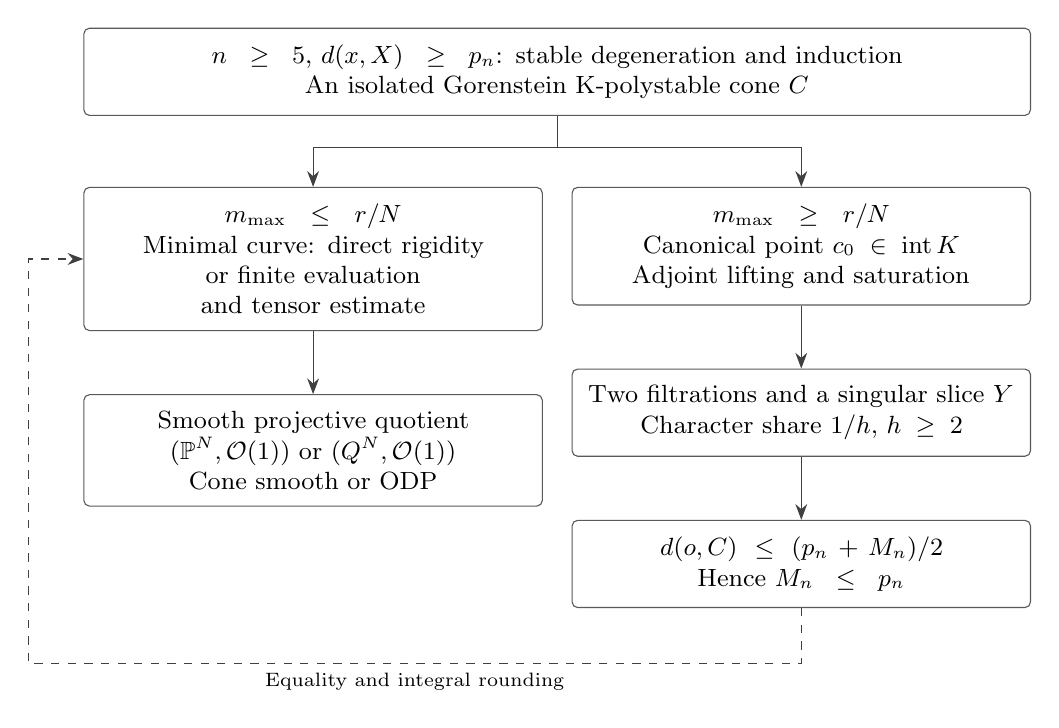
\begin{tikzpicture}[
  proofbox/.style={draw=black!65,rounded corners=2pt,align=center,
    inner sep=6pt,font=\small,text width=5.4cm},
  proofarrow/.style={-{Stealth[length=2mm]},draw=black!75},
  node distance=8mm and 8mm]
\node[proofbox,text width=11.6cm] (cone)
  {\(n\ge5\), \(d(x,X)\ge p_n\): stable degeneration and induction\\
   An isolated Gorenstein K-polystable cone \(C\)};
\node[proofbox,below=9mm of cone.south,xshift=-31mm] (small)
  {\(m_{\max}\le r/N\)\\
   Minimal curve: direct rigidity\\
   or finite evaluation and tensor estimate};
\node[proofbox,below=9mm of cone.south,xshift=31mm] (large)
  {\(m_{\max}\ge r/N\)\\
   Canonical point \(c_0\in\Int K\)\\
   Adjoint lifting and saturation};
\node[proofbox,below=8mm of small] (classify)
  {Smooth projective quotient\\
   \((\PP^N,\cO(1))\) or \((Q^N,\cO(1))\)\\
   Cone smooth or ODP};
\node[proofbox,below=8mm of large] (slice)
  {Two filtrations and a singular slice \(Y\)\\
   Character share \(1/h\), \(h\ge2\)};
\node[proofbox,below=8mm of slice] (bound)
  {\(d(o,C)\le (p_n+M_n)/2\)\\
   Hence \(M_n\le p_n\)};
\draw[proofarrow] (cone.south) -- ++(0,-4mm) -| (small.north);
\draw[proofarrow] (cone.south) -- ++(0,-4mm) -| (large.north);
\draw[proofarrow] (small) -- (classify);
\draw[proofarrow] (large) -- (slice);
\draw[proofarrow] (slice) -- (bound);
\coordinate (returnleft) at ($(small.west)+(-7mm,0)$);
\coordinate (returnbase) at ($(bound.south)+(0,-7mm)$);
\coordinate (returnturn) at (returnleft |- returnbase);
\draw[proofarrow,dashed] (bound.south) -- (returnbase)
  -- node[midway,below,font=\scriptsize]
     {Equality and integral rounding} (returnturn)
  -- (returnleft) -- (small.west);
\end{tikzpicture}

\caption{The induction step \(n=N+1\ge5\) for a singular germ of
density at least \(p_n\). Here \(K\) is the cone of leading Taylor
indices and \(c_0\) its canonical lattice point.
The same-dimensional slice enters only through the supremum \(M_n\)
of singular \(n\)-dimensional densities.
Equality in the volume estimate returns the cone to the small
stabilizer case.}
\label{fig:route}
\end{figure}

\paragraph{Organization.}
Section~\ref{sec:cones} fixes the valuation conventions, supplies the
cone reduction, and proves the absolute grading approximation.
Section~\ref{small:section} treats small stabilizers. For the other
case, Section~\ref{jet:section} proves canonical interiority and
Section~\ref{adj:section} independently establishes adjoint lifting
before combining the two results. Section~\ref{filt:section}
constructs the two filtrations and the second stabilizer.
Section~\ref{boot:section} constructs the same-dimensional singular
slice, proves the supremum inequality, and analyzes equality.
Finally, Section~\ref{sec:conclusion} returns to the original germ
and derives the Fano consequences.

\section{Normalized volume and the cone reduction}\label{sec:cones}

\subsection{Conventions and public inputs}

All varieties and stacks in the proof are over \(\CC\). Boundaries
are zero unless a boundary is explicitly introduced in a vanishing
argument. For a klt germ \(x\in X\), write \(R=\cO_{X,x}\) and
\(\fm=\fm_x\). If \(E\) is a prime divisor on a smooth proper
birational model \(\mu\colon X'\to X\), its log discrepancy is
\[
 A_X(E)=1+\operatorname{coeff}_E(K_{X'}-\mu^*K_X).
\]
For a real valuation \(v\) of \(K(X)\), trivial on \(\CC\) and
centered exactly at \(x\), put
\[
 \fa_t(v)=\{f\in R:v(f)\ge t\},\qquad
 \vol(v)=\lim_{t\to\infty}
     \frac{n!\,\length(R/\fa_t(v))}{t^n}.
\]
The ideals are \(\fm\)-primary. The limit exists by
\cite[Theorem~5.8]{Cutkosky13}: the local rings here are analytically
unramified and equicharacteristic with perfect residue field. The
integer-cutoff ideals form a graded family, and monotonicity extends
the integer limit to real cutoffs.

We use the standard extension of log discrepancy to real valuations.
On a smooth birational log model it is linear on each monomial cone;
for an arbitrary valuation it is the supremum over its monomial
retractions \cite[Proposition~5.1 and Corollary~5.4]{JM12}.
For the singular \(\QQ\)-Gorenstein base one includes the relative
canonical correction on a resolution, as in
\cite[Section~2.1]{Li18}. Define
\[
 \nvol_X(v)=
 \begin{cases}
 A_X(v)^n\vol(v),&A_X(v)<+\infty,\\
 +\infty,&A_X(v)=+\infty.
 \end{cases}
\]
Thus the definition never requires multiplying infinity by zero.
Our normalization is
\begin{equation}\label{cone:eq-density}
 \nvol(x,X)=\inf_v\nvol_X(v),\qquad
 d(x,X)=\frac{\nvol(x,X)}{n^n}.
\end{equation}
The infimum is unchanged if restricted to positive multiples of
divisorial valuations \cite[Theorem~2.5]{LiXu18}.
Rescaling a valuation does not change its
normalized volume.

We use the following established facts in their boundary-zero form.
\begin{enumerate}[label=(\roman*)]
\item A klt germ has a minimizing valuation, unique up to positive
scaling. It has finite discrepancy, is quasi-monomial, and has
finitely generated associated graded. The latter is a K-semistable
Fano cone, which admits a special equivariant degeneration to a
K-polystable Fano cone. The minimizing Reeb vector and normalized
volume are preserved \cite[Theorem~1.2]{XZStable},
\cite[Theorem~1.2]{LWX21}. Uniqueness also implies that a minimizer
normalized by discrepancy is invariant under every automorphism of
the germ \cite[Theorem~1.1 and Corollary~1.2]{XZ21}.
\item Normalized volume is lower semicontinuous in
\(\QQ\)-Gorenstein flat families of klt germs with section over a normal base
\cite[Theorem~1]{BL21}. In particular it is lower semicontinuous
when the point moves along a curve in a fixed klt variety
\cite[Theorem~33(1)]{BL21}. One has
\(d(x,X)\le1\), with equality exactly at smooth points
\cite[Theorem~1.6]{LX19}.
\item For a finite Galois morphism of klt germs
\(f\colon (Y,y)\to(X,x)\), with \(f^{-1}(x)=\{y\}\) set-theoretically
and \(K_Y=f^*K_X\), the finite degree formula is
\begin{equation}\label{cone:eq-cover}
              \nvol(y,Y)=\deg(f)\nvol(x,X).
\end{equation}
We use this only for a quotient by a group without reflections and
for the cyclic canonical index cover
\cite[Theorem~1.3]{XZ21}.
\item Isomorphic completed local rings have the same normalized
volume \cite[Lemma~2.15]{Liu22}. Thus étale germs at complex closed
points have the same invariant.
\end{enumerate}
These facts concern arbitrary klt germs. In particular, the first
item does not require a divisorial minimizer, isolatedness, or
smoothability.

\subsection{Products and embedding dimension}

\begin{lemma}[A smooth factor]\label{cone:product}
Let \(y\in Y\) be an \(N\)-dimensional klt germ, where \(N\ge1\). Then
\[
          d((y,0),Y\times\A^1)\le d(y,Y).
\]
\end{lemma}

\begin{proof}
Take a divisorial test \(v\) centered at \(y\), of discrepancy
\(A>0\) and volume \(\sigma\), and let \(a=A/N\).
The Gauss extension to the added parameter \(t\) is
\[
       (v\oplus a)\left(\sum_i f_it^i\right)
                    =\min_i\{v(f_i)+ia\}.
\]
On a log resolution this is a monomial valuation along the divisor
of \(v\) and \(t=0\), so its log discrepancy is \(A+a\).
Completion does not change the finite colengths. In the power-series
ring the quotient decomposes by powers of \(t\), giving
\[
 \length\bigl(R[[t]]/\fa_k(v\oplus a)\bigr)
   =\sum_{0\le i<k/a}\length\bigl(R/\fa_{k-ia}(v)\bigr).
\]
The defining asymptotic for \(\sigma\), followed by a Riemann sum,
gives \(\vol(v\oplus a)=\sigma/a\). Therefore
\[
 \frac{(A+A/N)^{N+1}}{(N+1)^{N+1}}\frac{N\sigma}{A}
                   =\frac{A^N\sigma}{N^N}.
\]
Take the infimum over the divisorial tests on \(Y\).
\end{proof}

\begin{lemma}[Lifting generators]\label{cone:edim}
Let \(v\) be a finite-discrepancy valuation of a klt germ, with
finitely generated positively graded associated graded ring
\(\gr_v R\). Then
\[
                \edim(R)\le\edim(\gr_v R).
\]
\end{lemma}

\begin{proof}
Choose minimal homogeneous algebra generators
\(\bar f_1,\ldots,\bar f_e\) of \(\gr_v R\), all of positive value,
and lift them to \(f_1,\ldots,f_e\in\fm\). To show that their
classes span \(\fm/\fm^2\), start with \(g\in\fm\). Its initial
form is a homogeneous polynomial in the \(\bar f_i\). Subtracting
the corresponding polynomial in the \(f_i\) either annihilates
the remainder or strictly increases its value. Every positive
value that occurs belongs to the semigroup generated by the
positive numbers \(v(f_i)\), so only finitely many such values
lie below any fixed bound.

The Izumi inequality for a finite-discrepancy valuation on a klt
germ \cite[Theorem~3.1]{Li18} gives
\(v(g)\le c\,\ord_{\fm}(g)\), with a fixed constant
\(c\). In particular, a nonzero remainder of value greater than
\(c\) lies in \(\fm^2\). The cancellation process therefore
terminates modulo \(\fm^2\) after finitely many steps. Every
polynomial subtracted has no constant term, and modulo
\(\fm^2\) is a linear combination of the \(f_i\). This proves
the assertion.
\end{proof}

\subsection{The minimum at the ordinary double point}

\begin{lemma}[The ODP minimum]\label{end:odp-value}
For \(n\ge2\), the ordinary double point \(Q_n\) has
\[
                           \nvol(0,Q_n)=2(n-1)^n.
\]
\end{lemma}

\begin{proof}
First take the exact quadratic cone
\[
 Q_n=\Spec R,\qquad
 R=\CC[z_0,\ldots,z_n]/(z_0^2+\cdots+z_n^2),
\]
with its ordinary grading. It is klt. For example, blowing
up the vertex resolves it with smooth exceptional quadric,
whose log discrepancy is \(n-1>0\); further smooth
blowups preserve the klt condition.

Normalize a minimizing valuation \(v\) by its discrepancy.
Uniqueness makes it invariant under all automorphisms,
in particular under cone scalings and the connected
orthogonal group \(\operatorname{SO}(n+1,\CC)\).
For each \(j\ge0\), the degree-\(j\) piece \(R_j\) is
the irreducible representation of complex harmonic polynomials
of degree \(j\) in \(n+1\) variables. To identify the quotient,
write \(P_j\) for homogeneous complex polynomials of degree \(j\)
and \(\mathcal H_j\) for the subspace killed by
\(\sum_i\partial_{z_i}^2\); set \(P_k=0\) for \(k<0\).
For \(q=\sum z_i^2\), the harmonic decomposition
\(P_j=\mathcal H_j\oplus qP_{j-2}\) identifies \(R_j\) with
\(\mathcal H_j\); see
\cite[Example~251 and Theorem~257]{GrahamSwansonMatthews15}.
The complex representation is irreducible already under the compact
group \(\operatorname{SO}(n+1)\), so an invariant subspace under
\(\operatorname{SO}(n+1,\CC)\) must be trivial or the whole space.
For the classical harmonic-polynomial formulation and its extensions,
see also \cite[Section~1]{LuoXu12}.
This includes \(n=2\) and \(n=3\).
The exception for two ambient variables is outside
the range under consideration.

For each cutoff \(t\), the subspace
\(\{f\in R_j:v(f)\ge t\}\) is invariant, so it is
either zero or all of \(R_j\). Every nonzero element of
\(R_j\) consequently has a common value \(a_j\).
If \(0\ne f\in R_1\), then \(f^j\ne0\), and
valuation multiplicativity gives \(a_j=j a_1\).
Invariance under cone scalings separates homogeneous
pieces of a cutoff: a finite Vandermonde combination
of scalings isolates each piece. Thus, for
\(g=\sum_j g_j\ne0\),
\[
                       v(g)=a_1\min\{j:g_j\ne0\}.
\]
After localizing at the vertex the same assertion
holds, since denominators nonzero at the vertex have
value zero. The minimizer is therefore proportional
to the ordinary degree valuation.

That valuation is the order along the exceptional
quadric of the vertex blowup. Hypersurface adjunction
gives discrepancy \(n-1\), and its volume is the
hypersurface multiplicity \(2\). It follows that the
infimum equals \(2(n-1)^n\).

Finally, an analytic ordinary double point has the
same completed local ring as this exact cone.
Completion invariance \cite[Lemma~2.15]{Liu22}
gives the same normalized volume.
\end{proof}

\subsection{The induction setup}

The companion paper \emph{The normalized-volume gap in dimension four}
\cite[Theorem~1.1]{FourfoldCompanion} proves the following base case.
We state the entire interface because its equality assertion is part
of the theorem propagated here.

\begin{theorem}[The fourfold gap]\label{inp:fourfold}
Let \(x\) be a singular closed point of a normal complex algebraic
fourfold \(X\). Suppose that \(K_X\) is \(\QQ\)-Cartier and \(X\) is klt
near \(x\), with zero boundary. Then
\[
                  \nvol(x,X)\le162.
\]
Equality holds if and only if the complex analytic germ is
\[
       \left(\{z_0^2+z_1^2+z_2^2+z_3^2+z_4^2=0\},0\right).
\]
No isolatedness, complete-intersection, quotient, or smoothability
assumption is made.
\end{theorem}

For \(k\ge2\) set
\begin{equation}\label{cone:eq-threshold}
              p_k=2\left(\frac{k-1}{k}\right)^k.
\end{equation}
Let \(M_k\) be the supremum of \(d(x,X)\) over all singular
boundary-zero klt \(k\)-fold germs: the varieties are normal and
complex algebraic, and their canonical divisors are
\(\QQ\)-Cartier. This supremum is finite, since \(M_k\le1\).
The numbers \(p_k\) are strictly increasing: for real \(t>1\),
\[
 \frac{d}{dt}\left[t\log(1-1/t)\right]
   =\log(1-1/t)+\frac1{t-1}>0.
\]
The last inequality is \(\log(1+u)<u\), with \(u=1/(t-1)\).

The dimension-two case of Theorem~\ref{thm:main} follows from
the quotient classification of klt surface singularities
\cite[Proposition~6.11]{CKM88}. The germ is analytically isomorphic to
\((\A^2/G,0)\), where \(G\) is a finite effective linear group
acting without reflections. Analytic isomorphism identifies the
completed local rings, so completion invariance transfers the
normalized volume to this algebraic quotient. The finite
degree formula gives \(d=1/|G|\). If the germ is singular,
\(|G|\ge2\), and equality with \(p_2=1/2\) forces an order-two
action without a fixed hyperplane, namely \((-1,-1)\).
This is the \(A_1\) surface singularity. The threefold case is
\cite[Theorem~1.3(1)]{LX19}, and the fourfold case is
Theorem~\ref{inp:fourfold}.

Henceforth, until the induction is closed, assume
Theorem~\ref{thm:main} in dimensions below \(n\), and fix
\begin{equation}\label{cone:eq-induction}
 n=N+1\ge5,\qquad
 d(x,X)\ge p_n,
\end{equation}
with \(x\) singular. The only use of \(M_n\) will be its definition
as a supremum, not an unproved upper bound in dimension \(n\).

\begin{proposition}[Cone reduction]\label{cone:reduction}
Under \eqref{cone:eq-induction}, there is a singular
K-polystable Fano cone \(C=\Spec S\), with vertex \(o\), such that
\[
 d(o,C)=d(x,X),\qquad
 \edim(X,x)\le\edim(C,o).
\]
The puncture \(C\setminus\{o\}\) is smooth, \(S\) is a normal
Gorenstein ring, and its canonical module has a homogeneous
generator. The cone has zero boundary.
\end{proposition}

\begin{proof}
Apply stable degeneration to a minimizer at \(x\), and then take
the K-polystable special degeneration. In the first passage the
induced Reeb valuation has the same volume and discrepancy as the
original minimizer \cite[Lemma~4.10]{LiXu18}.
In the second, equivariant flatness preserves the dimensions of
the character spaces and hence the Reeb volume. The relative
canonical character is constant, so its discrepancy is also
preserved. Li--Xu's characterization of K-semistability
\cite[Theorem~1.3]{LiXu18} shows that the final Reeb valuation
minimizes normalized volume over all centered valuations. Thus the two passages
preserve the infimum in \eqref{cone:eq-density}, not only the
number of an arbitrary test.

Lemma~\ref{cone:edim} gives the embedding-dimension inequality
for the first passage. Upper semicontinuity along the vertex
section of the special flat degeneration gives it for the
second. The final vertex is therefore singular.

Choose any positive integral grading of \(S\), and let \(P\ne o\).
Its grading orbit specializes to \(o\), so lower semicontinuity
gives
\begin{equation}\label{cone:eq-orbit-density}
                         d(o,C)\le d(P,C).
\end{equation}
Choose a homogeneous function \(f\), of degree \(d>0\), with
\(c=f(P)\ne0\), and put \(Y_P=\{f=c\}\subset C_f\).
The action map
\[
 Y_P\times\Gm\longrightarrow C_f,\qquad (Q,a)\longmapsto a\cdot Q,
\]
is the finite étale cover obtained by adjoining a root
\(a^d=f/c\). Near \((P,1)\), it expresses the germ as the product
of the \(N\)-dimensional slice \((Y_P,P)\) and a smooth curve.
The slice is klt by this étale description.
If \(P\) were singular, the slice would be
singular as well. The induction hypothesis,
Lemma~\ref{cone:product}, and étale invariance would then imply
\[
              d(P,C)\le p_N<p_n\le d(o,C),
\]
contrary to \eqref{cone:eq-orbit-density}. Thus the puncture is
smooth.

Let \(q\) be the canonical index at \(o\). The cyclic index
cover has degree \(q\), is quasi-étale and crepant, and is klt.
It has one point over \(o\). Indeed, its algebra is the direct
sum of the reflexive canonical powers modulo \(q\).
If a homogeneous element of a nonzero residue degree were
not nilpotent in the fiber over \(o\), a power returning to
degree zero would be a unit. The corresponding section would
trivialize a proper positive canonical power, contradicting
minimality of \(q\). Thus the nonzero residue-degree pieces
are nilpotent, and the reduced fiber consists of one point.
Equation~\eqref{cone:eq-cover} and the upper bound \(d\le1\)
give \(d(o,C)\le1/q\). Since \(p_n>1/2\), necessarily \(q=1\).

Klt singularities are Cohen--Macaulay
\cite[Definition~117 and Theorem~120]{KollarCanonicalModels10}.
The canonical module
\(\omega_S\) is invertible at the vertex, and a homogeneous
element generating its one-dimensional fiber there generates
it after localization. Its graded cokernel has empty support:
any nonempty closed support invariant under a positive
grading contains the vertex. Since \(\omega_S\) is torsion-free,
the resulting map \(S\to\omega_S\) is injective as well.
It is therefore an isomorphism, with a grading shift.
\end{proof}

\subsection{Integral gradings and orbifold quotients}

Fix the cone of Proposition~\ref{cone:reduction}. Let \(\mathbb T\)
be an effective algebraic torus of automorphisms containing its
Reeb vector \(\xi\), and normalize
\[
                              A(\xi)=n.
\]
Choose a \(\mathbb T\)-eigen-generator \(\Omega_C\) of
\(\omega_S\). Its character pairs with cocharacters as the
linear discrepancy functional \(A\)
\cite[Lemmas~2.16 and~2.18]{LiXu18}. Function weights use the
convention \(g(aP)=a^j g(P)\); the differential \(dg\) has the
same weight. The Reeb cone consists of cocharacters positive
on all nonconstant homogeneous functions.

\begin{lemma}[Fast primitive approximations]\label{cone:approximation}
There are primitive positive integral cocharacters \(\zeta_i\),
of canonical weights \(r_i=A(\zeta_i)\in\ZZ_{>0}\), such that
\begin{equation}\label{cone:eq-fast}
             \zeta_i=\frac{r_i}{n}\xi+\epsilon_i,\qquad
             \epsilon_i\longrightarrow0
\end{equation}
in the real cocharacter space. If the ray of \(\xi\) is
rational, the sequence may be chosen constant and exact.
Otherwise \(r_i\to\infty\).

The normalized volumes of the degree valuations
\(\wt_{\zeta_i}\) tend to \(\nvol(o,C)\).
For any fixed finite set of homogeneous algebra generators,
their \(\zeta_i\)-degrees lie between \(cr_i\) and \(Cr_i\)
for positive constants \(c,C\). Consequently the largest
stabilizer order \(m_{\max,i}\) on the puncture is \(O(r_i)\).
\end{lemma}

\begin{proof}
In the quotient of real cocharacter space by its integral
lattice, recurrence gives \(t_i\to\infty\) and integral
cocharacters \(q_i\) with \(q_i=t_i\xi+e_i\), where \(e_i\to0\).
One may obtain such a sequence from simultaneous Dirichlet
approximation, or from returns to zero of the one-parameter
subgroup in its compact closure. Let \(d_i\) be the gcd of
\(q_i\) in a lattice basis and put \(\zeta_i=q_i/d_i\).
Then
\[
 \zeta_i-\frac{A(\zeta_i)}n\xi
       =\frac1{d_i}\left(e_i-\frac{A(e_i)}n\xi\right)\longrightarrow0.
\]
The cocharacters are positive for large \(i\).
If their positive integers \(r_i=A(\zeta_i)\) had a bounded
subsequence, \eqref{cone:eq-fast} would make \(\zeta_i\)
bounded on that subsequence. A constant lattice subsequence
would then give \(\zeta=(r/n)\xi\), forcing the ray to be
rational. The rational case is handled by its primitive
generator.

Choose homogeneous algebra generators \(g_1,\ldots,g_a\)
with \(\mathbb T\)-characters \(\chi_1,\ldots,\chi_a\).
Each \(\langle\chi_j,\xi\rangle\) is positive, so
\eqref{cone:eq-fast} gives the asserted two-sided bounds
for their integral degrees. More precisely, the normalized
cocharacters \((n/r_i)\zeta_i\) converge to \(\xi\).
Uniform comparison on the finite set of generator characters
then compares their values on every occurring character:
each is a sum of generator characters with nonnegative
integer coefficients. It follows that the valuation ideals
of the normalized degree valuations are squeezed between
those of \(\wt_\xi\) with cutoff factors tending to one.
Their volumes therefore converge; their discrepancies are
all \(n\).

At a nonvertex point some generator is nonzero. Its
stabilizer for a primitive grading is cyclic, and its order
divides the degree of every nonvanishing generator. It is
therefore at most the largest generator degree, proving
the final assertion.
\end{proof}

In what follows, \emph{sufficiently fast gradings} always means
gradings in a sequence as in Lemma~\ref{cone:approximation},
including the exact constant sequence on a rational ray.
All constants may depend on the fixed cone. No uniformity
over the class defining \(M_n\) is asserted or needed.

\begin{lemma}[The quotient orbifold]\label{cone:orbifold}
For a primitive positive integral grading \(\zeta\), of
canonical weight \(r\), let
\[
          B=[(C\setminus\{o\})/\Gm].
\]
Then \(B\) is a smooth effective proper orbifold of dimension
\(N\), with projective coarse space \(\Proj S\).
It has a faithful ample weight-one line bundle \(L\) such that
\begin{equation}\label{cone:eq-section-ring}
         S_j=H^0(B,jL),\qquad -K_B=rL.
\end{equation}
Every stabilizer is a finite cyclic group. At a point of
order \(m\), a smooth transverse uniformizer carries a
faithful \(\mu_m\)-action, and \(L\) has a faithful fiber
character.
\end{lemma}

\begin{proof}
The smooth puncture has finite stabilizers for the positive
grading, so its quotient stack is smooth and Deligne--Mumford.
It is the usual stack associated with a positively graded
affine ring away from its vertex; its coarse space is
\(\Proj S\), and a sufficiently divisible positive power of
the weight-one line descends to an ample coarse line bundle.
This also proves properness.

The grading is effective because the integral cocharacter
is primitive in an effective torus. At a point, the finite
stabilizer acts trivially on the tangent line of the orbit.
If an element acted trivially also on a transverse tangent
space, it would have identity differential on the smooth
puncture. A finite-order automorphism in characteristic zero
is formally linearizable at a fixed point; hence that
element would be the identity on a neighborhood and thus
on the irreducible cone, contrary to effectiveness.
This proves faithfulness of the transverse representation
and effectiveness of the orbifold. The weight-one character
of the subgroup of \(\Gm\) is faithful by construction.

Sections of \(jL\) are the homogeneous functions of degree
\(j\) on the puncture. Normality and the codimension of the
vertex extend them to \(C\), giving the first equality in
\eqref{cone:eq-section-ring}. Contracting \(\Omega_C\)
with the Euler field gives a horizontal top form of
character \(r\), so \(K_B=-rL\).
\end{proof}

We retain the stack \(B\), its faithful line \(L\), and the
character information throughout the argument. In particular,
we do not replace \(L\) by a coarse line bundle before the
stabilizers have been shown to be trivial.

\section{Small stabilizers}
\label{small:section}

We use Proposition~\ref{cone:reduction} and
Lemmas~\ref{cone:approximation} and~\ref{cone:orbifold}.  Thus
\(C=\Spec S\) is a normal Gorenstein Fano cone of dimension \(n=N+1\),
where \(N\geq4\), its puncture \(C^\circ=C\setminus\{o\}\) is smooth,
and the polarized cone \((C,\xi)\) is K-polystable, with minimizing
Reeb vector normalized by \(A(\xi)=n\).  Fix homogeneous torus eigenfunctions
\(f_1,\ldots,f_q\) generating \(S\), with torus characters
\(\alpha_1,\ldots,\alpha_q\).  For a primitive positive integral grading
\(\zeta\), write
\[
 r=A(\zeta),\qquad
 B=[C^\circ/\Gm],\qquad -K_B=rL.
\]
Here \(L\) is the faithful ample orbifold line bundle of weight one.
The maximum stabilizer order for this grading is denoted by
\(m_{\max}\).  All constants in this section may depend on the fixed cone,
its torus and the displayed generators.

\begin{theorem}[Small-stabilizer classification]
\label{small:classification}
Let \(\zeta_i\) be primitive positive integral gradings satisfying
\begin{equation}
 \zeta_i=\frac{r_i}{n}\xi+\epsilon_i,
 \qquad r_i=A(\zeta_i),\qquad \|\epsilon_i\|\longrightarrow0,
 \qquad m_{\max}(\zeta_i)\leq\frac{r_i}{N}.
 \label{small:fast-sequence}
\end{equation}
For all sufficiently large \(i\), every stabilizer is trivial and
\(r_i\in\{N,N+1\}\).  More precisely, the polarized quotient is
\[
 (B_i,L_i)\cong
 \begin{cases}
  (\PP^N,\cO_{\PP^N}(1)),&r_i=N+1,\\
  (Q^N,\cO_{Q^N}(1)),&r_i=N,
 \end{cases}
\]
where \(Q^N\subset\PP^{N+1}\) is a smooth quadric.  Consequently the cone
\(C\) is respectively smooth or an ordinary double point.  The assertion
includes the constant exact primitive grading when the ray of \(\xi\)
is rational.
\end{theorem}

We begin with a minimal orbifold rational curve.  Its tangent characters
either force \(r=N\) and trivial stabilizers, or its deformations yield a
finite evaluation map and hence a nonzero symmetric tensor of negative
weight.  A metric lower bound for homogeneous symmetric tensors, together
with an approximation estimate uniform in their rank, gives the remaining
rigidity.

\subsection{A minimal orbifold rational curve}

For the moment fix one primitive grading satisfying
\begin{equation}
 m_{\max}\leq r/N.
 \label{small:stabilizer-assumption}
\end{equation}
The orbifold \(B\) is smooth and effective, is proper with projective
coarse space, and has ample anticanonical bundle \(rL\).  We use the
orbifold rational-curve theorem of Li--Zhou
\cite[Proposition~2.6]{LZ25}.  In this setting it supplies a
representable nonconstant map from \(\PP(1,\ell)\), where the only
possible stack point is infinity, whose anticanonical degree plus the
inverse age at that point is at most \(\dim B+1\).  In particular its
anticanonical degree is at most \(n\).  No positivity assumption on
\(T_B\) is required for this assertion.

Choose a map of least positive \(L\)-degree among all representable
nonconstant maps of this form, allowing \(\ell=1\).  Such a minimum
exists: representability embeds the source stabilizer in a target
stabilizer, so the denominators of these degrees divide one of the
finitely many integers at most \(m_{\max}\).  Write
\[
 f:\PP(1,\ell)\longrightarrow B,
 \qquad f^*L\cong\cO(e),\qquad e>0,
\]
and let \(m\) be the stabilizer order of its value at infinity.
This endpoint order need not equal \(m_{\max}\).  Thus
\(\ell\mid m\), and minimality and the existence theorem give
\(re/\ell\leq n\).  On the other hand,
\(r/m\geq N\) by Equation~\eqref{small:stabilizer-assumption}.  Hence
\begin{equation}
 1\leq\frac{em}{\ell}
 =\frac{re/\ell}{r/m}
 \leq\frac{N+1}{N}<2.
 \label{small:primitive-curve-degree}
\end{equation}
The expression \(em/\ell\) is an integer.  We obtain
\begin{equation}
 e=1,\qquad \ell=m,
 \qquad N\leq r/m\leq n.
 \label{small:curve-range}
\end{equation}

Choose an identification \(f^*L\cong\cO(1)\).  Passing to its grading
torsor gives an equivariant map
\[
 F:\A^2\setminus\{0\}\longrightarrow C^\circ,
 \qquad F(t x,t^m y)=t\cdot F(x,y).
\]
Since \(\A^2\) is normal and \(C\) is affine, the coordinate functions
extend uniquely across the origin.  Thus \(F:\A^2(1,m)\to C\) is a
homogeneous polynomial map.  Set \(P=F(0,1)\); its stabilizer is
\(\mu_m\).  Conversely, a homogeneous map with no preimage of the
vertex outside the origin, and with this degree-one torsor
identification, gives a representable map to \(B\): its maps on source
inertia groups are the inclusions inherited from the identity
homomorphism of the grading groups.

\begin{lemma}[Deformations with a fixed lift]
\label{small:deformation}
Let \(b_1',\ldots,b_n'\in\{1,\ldots,m\}\) represent the characters of
\(\mu_m\) on \(T_{C,P}\), with the trivial character represented by
\(m\).  Every component through \(F\) of the scheme of homogeneous maps
\(F':\A^2(1,m)\to C\) satisfying \(F'(0,1)=P\) has dimension at least
\begin{equation}
 \chi=n+\frac rm-\sum_{j=1}^n\frac{b_j'}m.
 \label{small:chi}
\end{equation}
In particular this dimension is at least \(n\), except possibly when
\(r/m=N\) and the entire tangent action at \(P\) is trivial.
\end{lemma}

\begin{proof}
Homogeneous maps form an affine scheme of finite type: in fixed
homogeneous generators of \(S\), each coordinate of the map is a
polynomial of a specified weighted degree, and the relations of \(S\)
give polynomial equations in their finitely many coefficients.  The
condition of avoiding the vertex outside the origin is open, as may be
checked on the proper weighted line.  Near the given map, deformation
theory can therefore be performed entirely in the smooth target
\(C^\circ\).

Let \(E\) be the rank-\(n\) bundle on \(\PP(1,m)\) obtained by
descending \(F^*T_{C^\circ}\).  Its determinant is \(\cO(r)\), so
\(\deg E=r/m\).  We are deforming an equivariant map with its source
and its grading torsor fixed; equivalently, we are deforming a section
of the associated smooth bundle, with the canonical section obstruction
theory of \cite[Theorem~4.13 and Equation~(4.18)]{Webb22}.
There is no quotient by source
automorphisms or by changes of the torsor identification.  If
\(D_\infty\) denotes the residual gerbe at infinity, the tangent and
obstruction spaces for fixing its value are
\[
 H^0(\PP(1,m),E(-D_\infty)),\qquad
 H^1(\PP(1,m),E(-D_\infty)).
\]
Thus their Euler characteristic is a lower bound for the dimension of
every component through the map.

For completeness, orbifold Riemann--Roch here says
\(\chi(E)=n+\deg E-\operatorname{age}(E_\infty)\).
It follows by taking the coarse pushforward: locally diagonalizing at
the stack point subtracts the fractional character weights from the
degree, after which ordinary Riemann--Roch on \(\PP^1\) applies.
Restriction to \(D_\infty\) has Euler characteristic equal to the
dimension of the invariant fiber, because \(\mu_m\) is linearly
reductive.  Subtracting that invariant dimension is precisely the
effect of representing each trivial character by \(m\) instead of
zero.  The exact sequence for restriction to \(D_\infty\) therefore
gives Equation~\eqref{small:chi}.

Since \(\sum b_j'/m\leq n\), we have \(\chi\geq r/m\).  The Euler
characteristic \(\chi\) is an integer.  If \(r/m>N\), it is at least
\(N+1=n\).  If \(r/m=N\)
and some character is nontrivial, the inequality is strict and the
same conclusion follows.
\end{proof}

\subsection{Finite evaluation and its symmetric tensor}

Assume that the exception in Lemma~\ref{small:deformation} does not
occur.  Let \(H\) be the reduced closure of an irreducible component
of the open locus of maps avoiding the vertex outside the origin,
in the affine scheme of homogeneous maps with \(F'(0,1)=P\).
Then \(H\) is integral and
\begin{equation}
 \dim H\geq n.
 \label{small:H-dimension}
\end{equation}
Precomposition with \((x,y)\mapsto(a x,y)\) preserves the chosen
component because the acting group \(\Gm\) is connected.  It gives a
positive grading on \(H\): every coefficient involving \(x\) has positive weight,
whereas the coefficients involving only \(y\) are fixed by \(P\).
All maps contract to the same map obtained by deleting the terms
involving \(x\).  Consider the equivariant evaluation morphism
\begin{equation}
 \operatorname{ev}:H\longrightarrow C,
 \qquad F'\longmapsto F'(1,0).
 \label{small:evaluation}
\end{equation}

\begin{lemma}[Finite evaluation]
\label{small:finite-evaluation}
The morphism in Equation~\eqref{small:evaluation} is finite and
surjective.  Its fiber over \(o\) is supported at the unique contracted
map.
\end{lemma}

\begin{proof}
Take \(F_0\in H\) with \(F_0(1,0)=o\).  Choose a pointed curve in
\(H\) through \(F_0\), with general point in the locus avoiding the
vertex, and normalize it.  Its generic map gives a twisted stable
graph map to \(B\times\PP^1\): the second map is the coarse
identification of \(\PP(1,m)\) with \(\PP^1\), and infinity is marked.
This graph is stable even before any contraction because its second
map has degree one.  After a finite base change, properness of twisted
stable maps gives a limiting graph map
\cite[Theorem~4.3]{AOV11}.  The target is a tame proper smooth
Deligne--Mumford stack with projective coarse space, as required by
that theorem.

There is a unique component of the limiting coarse source of second
degree one.  It maps isomorphically to \(\PP^1\); call it the
horizontal component.  All other components form rational trees
attached to it, since the total arithmetic genus is zero.
The first map on the horizontal component is the coarse rational
map defined by \(F_0\), after cancellation of its basepoints.
Indeed the two maps agree on the open set where the limiting
homogeneous coordinates do not vanish simultaneously.

We spell out why a positive-degree tail occurs over the finite
basepoint \([1:0]\).  Choose a sufficiently divisible integer \(k\)
such that \(kL\) descends to a very ample bundle on the coarse space
of \(B\), and \(m\mid k\).  Its pullback along the original maps is
the coarse bundle \(\cO_{\PP^1}(k/m)\).  The limiting projective
coordinates are binary forms of that degree.  They have a common
zero at \([1:0]\), because \(F_0(1,0)=o\), and are not all zero,
because \(F_0(0,1)=P\ne o\).  Cancelling their common divisor loses
positive degree at \([1:0]\).  A general hyperplane avoiding the
value of the canceled map at that point has the lost positive number
of inverse-image points specializing there.  In the limiting stable
map these points cannot lie on the horizontal component.  They are
therefore accounted for by positive first degree on a tree over
\([1:0]\).  This also proves the degree assertion directly, without
making an assumption about components that might occur over
infinity.

Choose a terminal leaf of that tree.  It does not contain the
infinity marking, since its second image is \([1:0]\).  It has one
node and no markings.  If its first map had degree zero, it would be
constant in both factors and unstable: stability requires the induced
coarse map to be a Kontsevich stable map
\cite[Section~4]{AOV11}, and an unmarked constant terminal leaf has
only one special point. Hence its first degree is
positive.  Its normalization is a twisted rational curve with at
most one stack point: the only allowed stack points of a twisted
source are nodes and markings.  Projection from the product target
to \(B\) preserves representability, since \(\PP^1\) has trivial
inertia.  The leaf consequently gives a representable nonconstant
map \(\PP(1,\ell')\to B\) of the type used in the minimum.

Its \(L\)-degree is at least the original minimal degree \(1/m\).
Degree is additive on the limiting source and every component has
nonnegative \(L\)-degree, while the total degree is \(1/m\).
Thus this leaf consumes the full first degree.  The horizontal
component has first degree zero, and its constant value is the
coarse image of \(P\).  It follows that the image of the affine map
\(F_0\) lies in the closure of the grading orbit of \(P\).

The normalization of that orbit closure is \(\A^1\), with a
parameter of grading weight \(m\), normalized to have value one at
\(P\).  To see the weight, the gcd of the degrees of the coordinates
nonzero at \(P\) is its stabilizer order \(m\).  The map from the
normal source \(\A^2\) factors through this normalization: its
parameter is integral over the coordinate ring of the orbit curve
and hence regular on \(\A^2\).  The parameter pulled back along
\(F_0\) is a weighted homogeneous polynomial of degree \(m\), so it
has the form
\[
 y+c x^m.
\]
The coefficient of \(y\) is one because the value at \((0,1)\) is
fixed.  Evaluation at \((1,0)\) is the vertex only if \(c=0\).
Therefore the vertex fiber is supported at the single contracted map.

Finally, let \(R_H\) be the positively graded coordinate ring of
\(H\).  The preceding fiber statement says that
\(R_H/S_+R_H\) is finite dimensional.  Lift a homogeneous basis of
this quotient.  Induction on the positive degree shows that these
lifts generate \(R_H\) as an \(S\)-module; this is graded
Nakayama.  Thus evaluation is finite.  Its image is closed and has
dimension \(\dim H\geq n\), by Equation~\eqref{small:H-dimension}.
Since \(C\) is integral of dimension \(n\), the image is all of
\(C\), and \(\dim H=n\).
\end{proof}

\begin{lemma}[A tensor of negative integral weight]
\label{small:norm-tensor}
Let \(b\) be the degree of the finite evaluation in
Lemma~\ref{small:finite-evaluation}.  There is a nonzero algebraic
section
\[
 s\in H^0(C^\circ,\Sym^bT_{C^\circ})
\]
of integral-grading weight \(-bm\).
\end{lemma}

\begin{proof}
The source automorphisms
\((x,y)\mapsto(x,y+t x^m)\), for \(t\in\CC\), preserve the
homogeneous-map scheme, the fixed value at \((0,1)\), and its open
locus avoiding the vertex.  The connected additive group therefore
preserves the component \(H\).  Its vector field is nonzero: a
coordinate nonzero at \(P\) has a nonzero pure power of \(y\), whose
derivative under this action is nonzero in characteristic zero.
Differentiating evaluation gives a regular vector \(V\) along
evaluation over \(C^\circ\).  It is generically nonzero, since the
finite dominant evaluation is generically separable and hence has
injective differential on a nonempty smooth open set.  For a target
coordinate of degree \(d\), its component is
\(\partial_yF'(1,0)\), of coefficient-grading degree \(d-m\).
Thus \(V\), as a vector along evaluation, has derivation weight
\(-m\).

Over the generic point, take the symmetric product of the vectors
on all \(b\) sheets.  This gives a nonzero element of
\(\Sym^bT_{C^\circ}\) over \(\CC(C)\); the product, unlike the
ordinary trace, cannot cancel.  It is invariant under permutation
of the sheets and so descends to that field.  It is regular as
well.  On a smooth affine open set of \(C^\circ\) trivializing the
tangent bundle, the components of \(V\) lie in a finite algebra
over the base ring.  The coefficients of their symmetric product
are therefore integral over the base ring and lie in its fraction
field.  Normality of the base makes them regular.  This argument
does not require \(H\) to be normal; alternatively one can first
use its finite normalization.  The construction is equivariant
and multiplies weights by \(b\), giving weight \(-bm\).
\end{proof}

\subsection{A bound for homogeneous symmetric tensors}

The tensor just constructed has negative weight for the integral grading.
To exploit this, we first bound the Reeb weight of a homogeneous
symmetric tensor.  By the Fano cone
Yau--Tian--Donaldson theorem
\cite[Theorem~1.1 and Definitions~2.1--2.2]{CS19}, \(C^\circ\) carries a
Ricci-flat K\"ahler cone metric with Reeb vector \(\xi\).  The theorem
applies here because the puncture is smooth and the singularity is
Q-Gorenstein and klt.  The condition called K-stability in that reference
allows equality only for an isomorphic central fiber, and is the
K-polystability condition used here.  With \(A(\xi)=n\), the real
homothetic dilations have infinitesimal generator \(-J\xi\), and their
pullback multiplies the metric by the square of the dilation factor.

\begin{lemma}[Tensor weight bound]
\label{small:tensor-bound}
Let \(b\geq1\), and let \(s\) be a nonzero homogeneous algebraic section
of \(\Sym^bT_{C^\circ}\), of \(\xi\)-weight \(\tau\), with vector fields
weighted as derivations.  Then
\[
 \tau\geq-b.
\]
\end{lemma}

\begin{proof}
The Chern connection induced on \(\Sym^bT_{C^\circ}\) has zero mean
curvature: contraction of the curvature on \(T_{C^\circ}\) is Ricci
curvature, and contraction commutes with the induced tensor and symmetric
power operations.  Put \(u=|s|^2\).  The holomorphic Bochner formula and
Cauchy--Schwarz give, with a consistent positive complex-Laplacian
normalization,
\[
 \Delta u=|\nabla^{1,0}s|^2\geq0,
 \qquad |\partial u|^2\leq u\,\Delta u.
\]
Consequently \(\log(u+a)\) is subharmonic for each \(a>0\), and so is
\((u+a)^{p/2}\) for every \(p>0\), by the chain rule applied to the
increasing convex exponential function.  Letting \(a\) decrease to zero
shows that \(|s|^p\) is subharmonic in the distributional sense, including
across the zero set of \(s\).

Let \(\rho\) be the metric radial coordinate and \(M=\{\rho=1\}\) its
compact smooth link.  A contravariant tensor of rank \(b\) and derivation
weight \(\tau\) has norm of radial degree \(\tau+b\).  If
\(\tau+b<0\), choose \(p>0\) such that
\[
 d=p(\tau+b)\in(2-2n,0).
\]
Then \(|s|^p=\rho^d\phi\) for a nonnegative continuous function
\(\phi\) on \(M\) with positive integral.  The cone-Laplacian formula,
valid also distributionally, is
\[
 \Delta(\rho^d\phi)
 =\rho^{d-2}\bigl(d(d+2n-2)\phi+\Delta_M\phi\bigr).
\]
Integrating the angular term over \(M\) gives zero.  Testing
subharmonicity against a nonnegative radial function supported in an
annulus would therefore imply
\(d(d+2n-2)\int_M\phi\geq0\), which is impossible.  Thus
\(\tau+b\geq0\).
\end{proof}

\subsection{Uniform control of characters and the conclusion}

The tensor rank in Lemma~\ref{small:norm-tensor} can vary with the
grading.  The following estimate makes the approximation error
independent of that rank.

\begin{lemma}[Character estimate]
\label{small:character-estimate}
There is a constant \(c>0\) with the following property for all
sufficiently close gradings in Equation~\eqref{small:fast-sequence}.
If a nonzero rank-\(b\) tensor on \(C^\circ\) has integral-grading
weight \(-bm\), with \(m>0\), then it has a nonzero torus
eigencomponent of character \(\chi\) satisfying
\[
 \|\chi\|\leq cb.
\]
Consequently, if the tensor is as in
Lemma~\ref{small:norm-tensor}, then
\begin{equation}
 m\leq\frac rn+c\|\epsilon\|.
 \label{small:m-bound}
\end{equation}
\end{lemma}

\begin{proof}
For the fixed eigen-generators \(f_j\), positivity of \(\xi\) and
absolute convergence of the error give constants \(c_1,c_2>0\)
such that their integral degrees \(d_j=\alpha_j(\zeta)\) satisfy
\begin{equation}
 c_1r\leq d_j\leq c_2r
 \quad\text{for every }j.
 \label{small:generator-weights}
\end{equation}
These bounds include the exact rational grading.

The differentials \(df_j\) span the cotangent bundle of \(C^\circ\).
Pairing a symmetric tensor with all ordered \(b\)-tuples of these
differentials embeds its space of sections into a finite tuple of
regular functions on \(C^\circ\).  Normality extends these functions
over \(o\).  This also shows that the torus action on sections is
locally finite, so the tensor has a nonzero torus eigencomponent;
every such component retains its specified \(\zeta\)-weight.

Let \(\chi\) be the character of a nonzero component, and choose a
nonzero pairing with
\(df_{j_1}\otimes\cdots\otimes df_{j_b}\).  Its function has
character
\(\beta=\chi+\alpha_{j_1}+\cdots+\alpha_{j_b}\) and integral degree
\[
 0\leq d=-bm+d_{j_1}+\cdots+d_{j_b}\leq c_2rb.
\]
It has a polynomial lift in the generators consisting of monomials
of character \(\beta\), by torus equivariance of the polynomial
presentation of \(S\).  Each such monomial contains at most
\(d/(c_1r)\leq(c_2/c_1)b\) factors, by
Equation~\eqref{small:generator-weights}.  As the generator
characters are fixed, this proves \(\|\beta\|=O(b)\), and then
\(\|\chi\|=O(b)\), uniformly in the tensor, its rank and the
grading.

Put \(\tau=\chi(\xi)\).  The eigencomponent satisfies
Lemma~\ref{small:tensor-bound}, so \(\tau\geq-b\).  On the other
hand,
\[
 -bm=\chi(\zeta)=\frac rn\tau+\chi(\epsilon)
 \geq-\frac rn b-cb\|\epsilon\|.
\]
Dividing by \(b\) proves Equation~\eqref{small:m-bound}.
\end{proof}

\begin{proof}[Proof of Theorem~\ref{small:classification}]
For each grading choose the minimal curve and its stabilizer order
\(m\) as above.  If the exceptional case in
Lemma~\ref{small:deformation} occurs, then \(r/m=N\) and the
\(\mu_m\)-action on \(T_{C,P}\) is trivial.  Faithfulness of the
transverse tangent action implies \(m=1\), hence \(r=N\).
Equation~\eqref{small:stabilizer-assumption} then forces
\(m_{\max}=1\).

For the remaining indices, Lemmas~\ref{small:finite-evaluation}
and~\ref{small:norm-tensor} apply.  The character estimate and
Equation~\eqref{small:curve-range} give
\[
 0\leq nm-r\leq nc\|\epsilon\|.
\]
The left side is an integer.  Since the error tends to zero, we
have \(nm=r\) for all sufficiently large indices.  For a rational
ray with its constant exact grading the error is zero, so this
equality holds directly.

Now the finite evaluation has \(\dim H=n\), whereas its deformation
dimension satisfies
\[
 n=\dim H\geq n+\frac rm-\sum_{j=1}^n\frac{b_j'}m
 =2n-\sum_{j=1}^n\frac{b_j'}m\geq n.
\]
All equalities must hold.  In particular every \(b_j'=m\), so the
tangent action is trivial.  Its faithfulness again gives \(m=1\),
and now \(r=n=N+1\).  Finally
\[
 m_{\max}\leq\frac{N+1}{N}<2
\]
forces \(m_{\max}=1\).

The quotient is therefore an ordinary smooth projective Fano
\(N\)-fold and \(L\) an actual ample line bundle.  The
Kobayashi--Ochiai theorem in its ample-line-bundle formulation
\cite{KO73}, also supplied by \cite[Theorems~1.1 and~1.3]{ADK08}, applied to
\(-K_B=rL\) with \(r=N+1\) or \(N\), gives precisely the two
polarized varieties stated in the theorem.  The polarization is
the standard one, as also follows by substituting into their
Picard groups.  By the section-ring identity from the cone setup,
\[
 S=\bigoplus_{j\geq0}H^0(B,jL).
\]
This is the polynomial ring for \((\PP^N,\cO(1))\), and the
homogeneous coordinate ring of a nondegenerate quadratic
hypersurface for \((Q^N,\cO(1))\).  Its affine cone is respectively
smooth or the \(n\)-dimensional ordinary double point.
\end{proof}

\section{Jet cones and the canonical interior point}
\label{jet:section}

We work with the fixed cone supplied by
Proposition~\ref{cone:reduction}. Thus $C=\Spec S$ has dimension
$n=N+1$, its puncture is smooth, and its canonical module has a
homogeneous nowhere-vanishing generator on the puncture. The minimizing
Reeb vector $\xi$ is normalized by $A_C(\xi)=n$. Throughout this section,
\begin{equation}\label{jet:density-hypothesis}
 \nvol(o,C)\ge 2N^n.
\end{equation}
Take the primitive positive gradings of
Lemma~\ref{cone:approximation}, so that
\[
 \zeta_\nu=(r_\nu/n)\xi+\epsilon_\nu,
 \qquad r_\nu=A_C(\zeta_\nu),\qquad \epsilon_\nu\longrightarrow0
\]
in absolute cocharacter norm. In the rational case we use the exact
constant grading. Consider a subsequence on which the largest stabilizer
order satisfies $m_\nu\ge r_\nu/N$, and choose a point attaining that
order. We suppress the index $\nu$ when discussing a single grading.
Constants carrying a subscript $C$ may depend on this fixed cone and on
$N$; no uniformity over different cones is needed.

\subsection{Leading Taylor terms and the real cone}

Let $B$ and $L$ be the smooth quotient orbifold and its weight-one line
bundle from Lemma~\ref{cone:orbifold}. In particular,
\[
 S_j=H^0(B,jL),\qquad -K_B=rL.
\]
At the chosen point, take a smooth equivariant uniformizer with parameters
$z_1,\ldots,z_N$ and stabilizer $\mu_m$. Choose the parameters and the
frame of $L$ so that their characters are respectively
$b_1,\ldots,b_N\in\ZZ/m$ and $1$. We choose these algebraically:
averaging regular lifts of a cotangent eigenbasis gives an equivariant
map to $\A^N$ that is étale at the chosen point, and averaging a
nonvanishing local frame gives the specified line character.
After shrinking, these are equivariant algebraic étale coordinates
and an algebraic frame. A section of $jL$ is then represented
by a power series $F(z)$ satisfying
\[
 F(\varepsilon^{b_1}z_1,\ldots,\varepsilon^{b_N}z_N)
 =\varepsilon^j F(z).
\]
Order monomials first by total degree and then lexicographically, with
the smallest monomial first. Write $\operatorname{in}(s)=z^\gamma$ for
the leading monomial, omitting its nonzero scalar coefficient, and put
\begin{align}
 \Gamma&=\{(j,\gamma):0\ne s\in S_j,
                     \ \operatorname{in}(s)=z^\gamma\},
                     \label{jet:semigroup}\\
 \Lambda&=\{(j,\gamma)\in\ZZ\times\ZZ^N:
                  j\equiv\textstyle\sum_i b_i\gamma_i\pmod m\},
                     \label{jet:lattice}\\
 K&=\overline{\operatorname{cone}(\Gamma)}
                       \subset\RR\times\RR^N.
                     \label{jet:cone}
\end{align}
Here $(0,0)\in\Gamma$, and $\gamma=0$ denotes a nonzero constant Taylor
term, including those of sections of positive degree. The degree
coordinate in Equations~\eqref{jet:semigroup}--\eqref{jet:cone} is the
\emph{original} degree $j$.

For integrations only, introduce the scaled degree and the number
\begin{equation}\label{jet:scaling}
 s=\frac r{Nm}\le1,\qquad
 D_0=\frac{j}{sm}=\frac{Nj}{r}.
\end{equation}
We distinguish the coordinate $D_0$ from $j$ throughout. Write
$\widetilde K$, $\widetilde\Gamma$, and $\widetilde\Lambda$ for the
images of $K$, $\Gamma$, and $\Lambda$ under
$(j,x)\mapsto(Nj/r,x)$.

\begin{proposition}[Jet setup]\label{jet:setup}
The following assertions hold.
\begin{enumerate}[label=\textup{(\roman*)}]
\item
$\Gamma$ is an additive semigroup with one-dimensional leaves, and its
generated group is exactly $\Lambda$. Every finite compatible Taylor
jet is realized by sections of all sufficiently large degrees in each
admissible progression.
\item
$K$ is a full-dimensional closed convex cone, contains the positive
constant ray, projects onto the whole exponent orthant, and satisfies
$K=\overline{\Int K}$. Its bounded-degree sections are bounded. More
precisely, uniformly in the chosen point and nearby grading,
\begin{equation}\label{jet:bezout-bound}
 |\gamma|:=\sum_i\gamma_i\le C_C\frac jr
                       \qquad ((j,\gamma)\in K).
\end{equation}
Its scaled image has the form
\begin{equation}\label{jet:epigraph}
 \widetilde K=\{(D_0,x):x\in\RR_{\ge0}^N,\ D_0\ge f(x)\},
\end{equation}
where $f$ is finite, positively
homogeneous, convex, and
\begin{equation}\label{jet:f-coercive}
 f(x)\ge c_C|x|\qquad(x\in\RR_{\ge0}^N)
\end{equation}
for a constant $c_C>0$ independent of the nearby grading and chosen
point.
\item
In the scaled coordinates the lattice density is $s$. If $\ell$ is a
linear functional strictly positive on $\widetilde K\setminus\{0\}$, then
\begin{equation}\label{jet:count}
 \begin{aligned}
 &\#\{\gamma'\in\widetilde\Gamma:\ell(\gamma')<q\}\\
 &\qquad=s\,\operatorname{Leb}\{(D_0,x)\in\widetilde K:\ell(D_0,x)<1\}\,q^n+o(q^n),
 \end{aligned}
\end{equation}
with Lebesgue measure in the scaled coordinates. No saturation
assumption on $\Gamma$ is required.
\item
The vector
\begin{equation}\label{jet:canonical-vector}
 c_0=(r,\mathbf1)\qquad\text{in the original }(j,\gamma)
 \text{ coordinates}
\end{equation}
belongs to $\Lambda$. Its scaled coordinates are $(N,\mathbf1)$.
\end{enumerate}
\end{proposition}

\begin{proof}
Leading monomials multiply, and the associated leading coefficient is a
scalar. This proves additivity and the one-dimensional-leaf assertion.
In particular, each leading index in a fixed degree accounts for one
dimension of $S_j$.

Choose an integer $M>0$ divisible by all stabilizer orders such that
$ML$ descends to an ample line bundle on the coarse space. In a fixed
residue class $j_0$ modulo $M$, prescribe a finite compatible Taylor jet
of a section of $j_0L$. The kernel of the map to that finite jet space
is coherent. Serre vanishing after tensoring by sufficiently large
powers of $ML$, or after exact tame pushdown to the coarse space,
makes the map on global sections surjective. Thus the prescribed jet is
realized in every sufficiently large degree $j_0+kM$. Taking all the
finitely many admissible residue classes proves the assertion about
progressions. In particular, constants occur in all sufficiently large
degrees divisible by $m$, and each monomial $z^\gamma$ occurs as a
leading term in sufficiently large compatible degrees.

Differences of two such constant indices whose degrees differ by $m$
give $(m,0)$ in the generated group. For each $i$, a realized linear
jet gives an index $(j_i,e_i)$ with $j_i\equiv b_i\pmod m$.
The vectors $(m,0),(j_1,e_1),\ldots,(j_N,e_N)$ generate the full
congruence lattice in Equation~\eqref{jet:lattice}. All indices satisfy
that congruence, proving equality of groups. These same indices show
that the cone contains the positive constant ray, has full dimension,
and projects onto the exponent orthant.

We next prove the uniform estimate. Fix torus eigen-generators of $S$
and the resulting affine embedding of $C$. Their $\zeta_\nu$-degrees
are bounded below by a fixed positive multiple of $r_\nu$ for all
sufficiently large $\nu$, because their $\xi$-weights are positive.
A section of degree $j$ has a homogeneous polynomial lift in these
generators, of ordinary polynomial degree at most $Cj/r$. At a smooth
point of the punctured cone, a homogeneous function has the same local
vanishing order as its restriction to a transverse slice: in orbit and
slice coordinates it is a unit power of the orbit coordinate times its
slice expression.

Take a general complete-intersection curve through the smooth point,
cut out by affine hyperplanes in the fixed embedding. It is smooth
there and is not contained in the zero locus of the nonzero function.
The local intersection multiplicity with the function is at least its
local vanishing order. B\'ezout's inequality bounds this multiplicity
by the polynomial degree times the degree of the fixed embedded cone.
This proves Equation~\eqref{jet:bezout-bound} for $\Gamma$, and then for
$K$ by homogeneity and closure. In particular, bounded degree cuts are
compact.

The positive constant ray makes every nonempty fiber over an exponent
$x$ an upper ray in degree. Every exponent fiber is nonempty, since
nonnegative combinations of the indices $(j_i,e_i)$ reach every
$x\ge0$. Closedness and the degree bound make the lowest degree in each
fiber attainable. Hence $K$ is the epigraph of a finite convex
positively homogeneous function in the scaled coordinates.
Equation~\eqref{jet:bezout-bound} becomes
Equation~\eqref{jet:f-coercive}. A full-dimensional closed convex cone
is the closure of its interior.

The original lattice has covolume $m$. The coordinate change
$(j,\gamma)\mapsto(Nj/r,\gamma)$ multiplies covolumes by $N/r$;
the resulting covolume is $Nm/r=1/s$.
For clarity, we give the nonsaturated semigroup counting argument.
This is the conductor-and-exhaustion method for value semigroups
\cite[Theorems~1.4 and~1.6]{KavehKhovanskii2012}, also used for
graded linear series in \cite[Proposition~2.1]{LazarsfeldMustata2009}.
Its asymptotic conclusion does not assert exact saturation.
Let $\Gamma_0$ be a finitely generated subsemigroup with full generated
group $\Lambda$, and let $K_0$ be its cone. There is a vector
$c\in\Gamma_0$ such that
\begin{equation}\label{jet:conductor}
 c+(K_0\cap\Lambda)\subset\Gamma_0.
\end{equation}
Indeed every lattice point of $K_0$ lies in a cone generated by a
linearly independent subset of the finite generating set. Removing the
integer parts of its nonnegative coefficients writes it as a
semigroup element plus a lattice point in one of finitely many bounded
parallelepipeds. There are only finitely many possible remainders $v$.
Since the group is $\Lambda$, write each such remainder as
$v=v_+-v_-$ with $v_\pm\in\Gamma_0$. The sum of all the $v_-$ is a
single $c$ for which Equation~\eqref{jet:conductor} holds. Translating a
bounded linear cutoff changes its scale by a constant, so ordinary
lattice counting between $c+(K_0\cap\Lambda)$ and $K_0\cap\Lambda$
gives its leading lattice volume. After the coordinate change this
is Euclidean volume with density $s$.

Now exhaust $\Int K$ by cones of finitely many indices of $\Gamma$,
always retaining a fixed finite set whose group is $\Lambda$.
Every interior point belongs to the interior of one of these finite
cones: choose a small simplex surrounding it in $\Int K$ and
approximate the simplex vertices by elements of
$\operatorname{cone}(\Gamma)$. The resulting finite cones give the lower
leading count. Counting all lattice points of $K$ gives the upper
count. Compact convex cutoff bodies have boundary of Lebesgue measure
zero, and their volumes are exhausted from the interior. This proves
Equation~\eqref{jet:count}.

Finally, on the uniformizer the canonical character is the negative of
the sum of the coordinate characters, in the convention for equivariant
line bundles used here. The identity $-K_B=rL$ therefore gives
$r\equiv\sum_i b_i\pmod m$, proving
Equation~\eqref{jet:canonical-vector}.
\end{proof}

\subsection{Discrepancy and moment tests}

\begin{lemma}[The degree and Taylor-order test]\label{jet:test}
For $\delta\in\QQ_{\ge0}$, the rule
\begin{equation}\label{jet:test-rule}
 v_\delta\Bigl(\sum_j s_j\Bigr)
   =\min_{s_j\ne0}\left\{\frac{Nj}{r}
                           +\delta\ord_z(s_j)\right\}
\end{equation}
defines a valuation centered at the vertex. It is divisorial up to
positive rescaling, and
\begin{align}
 A_C(v_\delta)&=N+N\delta,\label{jet:test-discrepancy}\\
 A_C(v_\delta)^n\vol(v_\delta)
   &=N^n(1+\delta)^n s
        \int_{\RR_{\ge0}^N}e^{-f(x)-\delta|x|}\,dx.
                                      \label{jet:test-volume}
\end{align}
\end{lemma}

\begin{proof}
Use the local line-bundle extraction over the chosen uniformizer.
Write $t$ for its line coordinate, of grading weight one. Its finite
quotient presentation has the action
\[
 (t,z_1,\ldots,z_N)\longmapsto
 (\varepsilon^{-1}t,\varepsilon^{b_1}z_1,\ldots,
                                      \varepsilon^{b_N}z_N).
\]
A homogeneous function of degree $j$ pulls back to $t^jF_j(z)$.
The monomial valuation with costs
\[
 v(t)=N/r=1/(sm),\qquad v(z_i)=\delta
\]
therefore restricts to Equation~\eqref{jet:test-rule}. Distinct original
degrees have different powers of $t$, so even when scalar values agree
their lowest monomials cannot cancel. Rational positive costs give a
divisorial monomial valuation up to rescaling. At $\delta=0$ the rule is
the rescaled ordinary degree valuation. The positive degree cost and
the positivity of all algebra-generator degrees imply that its center
is the vertex.

Let $\Omega_C$ be the homogeneous canonical generator of weight $r$.
On this chart it has the form
\[
 t^{r-1}u(z)\,dt\wedge dz_1\wedge\cdots\wedge dz_N,
 \qquad u(0)\ne0.
\]
The exponent follows from homogeneity, and the coefficient is a unit
because $\Omega_C$ is nonvanishing on the punctured cone. Computing
discrepancy from this pulled-back form, including the finite-chart
ramification in the restricted value scaling, gives
\[
 A_C(v_\delta)=\frac Nr+N\delta+(r-1)\frac Nr
             =N+N\delta.
\]
Equivalently one can take a weighted monomial extraction on the smooth
chart and apply the canonical divisor formula there; the same
calculation descends to the quotient. For $\delta=0$ it is the canonical
degree formula.

In each $S_j$, a leading-term basis is compatible with total Taylor
order. Thus the colength below a cutoff $q$ is the number of indices
of $\Gamma$ satisfying $D_0+\delta|x|<q$. These finite quotients are
supported at the vertex, so computing them in $S$ or in its local ring
gives the same length. Proposition~\ref{jet:setup} applies to this
strictly positive cutoff functional. Since $K$ has dimension $n$,
homogeneity and integration by layers give
\[
 n!\operatorname{Leb}\{(D_0,x)\in\widetilde K:D_0+\delta|x|<1\}
 =\int_{\widetilde K}e^{-D_0-\delta|x|}\,dD_0\,dx
 =\int_{\RR_{\ge0}^N}e^{-f(x)-\delta|x|}\,dx.
\]
Combining this identity with the lattice density and
Equation~\eqref{jet:test-discrepancy} proves
Equation~\eqref{jet:test-volume}.
\end{proof}

Let $X_1,\ldots,X_N$ be independent exponential random variables of
mean one. For the current grading put
\begin{equation}\label{jet:moment-notation}
 B_0(x)=f(x)-|x|,\qquad
 H=\mathbb E e^{-B_0(X)}=\int_{\RR_{\ge0}^N}e^{-f(x)}\,dx.
\end{equation}

\begin{lemma}[The two moment inequalities]\label{jet:moments}
Along the fixed-cone sequence of gradings, there are numbers
$\eta_\nu\ge0$ tending to zero such that
\begin{equation}\label{jet:moment-inequalities}
 H\ge\frac2s,\qquad
 \mathbb E[(1+B_0(X))e^{-B_0(X)}]\ge-\eta_\nu H.
\end{equation}
For an exact minimizing rational grading one may take $\eta_\nu=0$.
\end{lemma}

\begin{proof}
Write $F(\delta)$ for the right side of
Equation~\eqref{jet:test-volume}. The volume hypothesis and the test at
zero give
\[
 2N^n\le\nvol(o,C)\le F(0)=N^n sH,
\]
which is the first inequality.

Consider the probability measure $d\mu_f=H^{-1}e^{-f(x)}dx$.
Positive homogeneity gives, for every $t>0$,
\[
 \int e^{-tf(x)}dx=t^{-N}H.
\]
Differentiating, justified by Equation~\eqref{jet:f-coercive}, yields
\begin{equation}\label{jet:homogeneous-moments}
 \mathbb E_{\mu_f}f=N,\qquad
 \mathbb E_{\mu_f}f^2=N(N+1).
\end{equation}
In particular,
\begin{align}
 \frac{F'(0)}{F(0)}
 &=n-\mathbb E_{\mu_f}|x|\notag\\
 &=1+\mathbb E_{\mu_f}(f-|x|)
 =\frac{\mathbb E[(1+B_0)e^{-B_0}]}{H}.
                                           \label{jet:first-derivative}
\end{align}

We check the uniformity needed for near-minimality.
Equation~\eqref{jet:f-coercive} and
Equation~\eqref{jet:homogeneous-moments} give uniform first and second
moments of $|x|$ under $\mu_f$. Indeed they are at most
$c_C^{-1}N$ and $c_C^{-2}N(N+1)$, respectively. Since
\[
 \frac{F(\delta)}{F(0)}
   =(1+\delta)^n\mathbb E_{\mu_f}e^{-\delta|x|},
\]
twice differentiating shows
\begin{equation}\label{jet:second-derivative}
 \sup_{0\le\delta\le1}\frac{|F''(\delta)|}{F(0)}\le C'_C
\end{equation}
for a fixed finite constant. The three terms are bounded by constant
multiples of $1$, $\mathbb E_{\mu_f}|x|$, and
$\mathbb E_{\mu_f}|x|^2$, because $e^{-\delta|x|}\le1$.

The test at zero is a rescaling of the current degree valuation, so
Lemma~\ref{cone:approximation} gives
$F_\nu(0)\to\nvol(o,C)$. If $F'_\nu(0)/F_\nu(0)$ were bounded above by
a fixed negative number along a subsequence, Taylor's formula and
Equation~\eqref{jet:second-derivative} would give a fixed small positive
rational $\delta$ and a fixed $\rho>0$ such that
$F_\nu(\delta)\le(1-\rho)F_\nu(0)$. This is incompatible with
$F_\nu(\delta)\ge\nvol(o,C)>0$ and the preceding convergence.
Thus $F'_\nu(0)/F_\nu(0)\ge-\eta_\nu$ for some $\eta_\nu\to0$.
Equation~\eqref{jet:first-derivative} proves the second inequality. At
an exactly minimizing degree valuation, every positive rational test
has volume at least $F(0)$, so its right derivative is nonnegative.
\end{proof}

\subsection{A uniform exponential expectation inequality}

We need to bound $H$ when $B_0$ is bounded below by a linear
function whose coefficients sum to zero. The second inequality in
Lemma~\ref{jet:moments} controls the expectation of $(1+B_0)e^{-B_0}$. Combining it with $H$
leads, for $u>0$, to $(1+(1+B_0)/u)e^{-B_0}$, whose pointwise upper envelope
is the truncated exponential below.

Define the continuously differentiable function
\begin{equation}\label{prob:g}
 g(y)=\begin{cases}
 1,&y\le0,\\
 (1+y)e^{-y},&y>0,
 \end{cases}
\end{equation}
Here $0\le g\le1$.

For any real $v$ and any $u>0$, elementary differentiation gives
\begin{equation}\label{jet:envelope}
 \sup_{b\ge v}\left(1+\frac{1+b}{u}\right)e^{-b}
       =\frac{e^u}{u}g(u+v).
\end{equation}
Indeed the derivative of the expression on the left before
maximization is $-(u+b)e^{-b}/u$, so its maximum is attained at
$b=-u$ when $v\le-u$, and at $b=v$ otherwise.

\begin{theorem}[The exponential bound]\label{prob:bound}
For $u=4/3$ one has
\begin{equation}\label{prob:universal-bound}
 \sup_{N\ge1}\ \sup_{\substack{a\in\RR^N\\\sum_i a_i=0}}
 \frac{e^u}{u}\mathbb E g(u+a\cdot X)
 =C_*:=\frac34e^{4/3}-\frac e3<2.
\end{equation}
The supremum over dimensions is approached by the vectors
$(2,-2/(N-1),\ldots,-2/(N-1))$ as $N\to\infty$.
\end{theorem}

The theorem gives a bound strictly below the threshold $2$ in
Lemma~\ref{jet:moments}. We prove it before applying it to the
canonical point. For the proof, put $h=1-g$; then
\begin{equation}\label{prob:kernel}
 h'(y)=ye^{-y}\mathbf1_{\{y>0\}},\qquad
 k(y):=h''(y)=(1-y)e^{-y}\mathbf1_{\{y>0\}}
\end{equation}
holds almost everywhere. In particular $h'$ is globally Lipschitz and
$k$ is bounded.

\begin{lemma}[Log-concavity and a barycenter half-space bound]
\label{prob:logconcavity}
A nonzero mean-zero linear combination of independent mean-one
exponentials has a positive continuous log-concave density on the whole
real line. Adding further independent scaled exponentials, with either
sign of coefficient, preserves these properties. If $Z$ has such a
density, then
\begin{equation}\label{prob:grunbaum}
 \frac1e\le\mathbb P(Z\le\mathbb EZ)\le1-\frac1e.
\end{equation}
\end{lemma}

\begin{proof}
The preservation of log-concavity under convolution is a special case
of the classical theory of Pr\'ekopa
\cite[Theorems~7--8]{Prekopa1973}; we give the elementary
exponential-specific argument needed here. A nonzero coefficient
vector with sum zero has a positive and a negative coefficient. The
difference $aE-bE'$ for $a,b>0$ has density
\[
 p(x)=\frac1{a+b}
 \begin{cases}e^{x/b},&x\le0,\\e^{-x/a},&x\ge0.
 \end{cases}
\]
It is positive, continuous, and log-concave.

Let $r$ be a positive log-concave function for which the indicated
one-sided integrals are finite. Set
$R(x)=\int_{-\infty}^x r(y)dy$. For $t\ge0$, concavity of $\log r$
implies that $r(x-t)/r(x)$ is nondecreasing in $x$. Thus
\[
 \frac{R(x)}{r(x)}=\int_0^\infty\frac{r(x-t)}{r(x)}dt
\]
is nondecreasing, and $(\log R)'=r/R$ is nonincreasing. Consequently
$R$ is log-concave. The same argument with $r(x+t)/r(x)$ shows that
$T(x)=\int_x^\infty r(y)dy$ is log-concave: $T/r$ is nonincreasing,
so $(\log T)'=-r/T$ is nonincreasing. These statements can equivalently
be read almost everywhere; the positive functions involved are locally
absolutely continuous.

If $p$ is a positive log-concave probability density, adding $cE$ or
$-cE$, $c>0$, produces respectively the densities
\[
 \frac{e^{-x/c}}c\int_{-\infty}^x e^{y/c}p(y)dy,
 \qquad
 \frac{e^{x/c}}c\int_x^\infty e^{-y/c}p(y)dy.
\]
The integrands are exponential tilts of $p$, hence log-concave, and
the appropriate one-sided integrals are finite. The preceding argument
proves log-concavity of the new densities. Positivity and continuity
are immediate from the displayed formulas. Induction starting with
$aE-bE'$ proves the assertions about finite exponential sums, and
translation does not affect them.

For completeness, Equation~\eqref{prob:grunbaum} is the
one-dimensional log-concave form of Gr\"unbaum's centroid inequality
\cite{Grunbaum1960}; see \cite[Lemma~5.4]{LovaszVempala2007} and
\cite[Section~3]{MNRY18}. It follows directly here from the same integral
argument. If $G$ is the distribution function of $Z$, both $G$ and
$1-G$ are log-concave. Since $G(Z)$ is uniform on $(0,1)$, Jensen's
inequality gives
\[
 \log G(\mathbb EZ)\ge\mathbb E\log G(Z)
 =\int_0^1\log t\,dt=-1.
\]
Applying the same reasoning to $1-G$ gives
$\log(1-G(\mathbb EZ))\ge-1$. All the means in the present application
are finite, and both logarithmic expectations just used equal $-1$.
These two inequalities give Equation~\eqref{prob:grunbaum}.
\end{proof}

\begin{lemma}[Strict single crossing]\label{prob:single-crossing}
Let $Z$ have a positive log-concave probability density on $\RR$, and
let $E$ be an independent mean-one exponential. If
\[
 \mathbb E k(Z+c_*E)=0,
\]
then $\mathbb E k(Z+cE)>0$ for every $c<c_*$ and
$\mathbb E k(Z+cE)<0$ for every $c>c_*$.
\end{lemma}

\begin{proof}
Write $p$ for the density of $Z$ and first consider
\[
 \psi(t)=\mathbb E k(Z+t)
        =\int_0^\infty(1-y)e^{-y}p(y-t)dy.
\]
This is continuous, by continuity of translation in $L^1$ and
boundedness of $k$. A positive log-concave density has a continuous
representative whose logarithm is finite and concave. For $t_1<t_2$,
the ratio
\[
 r(y)=p(y-t_2)/p(y-t_1)
\]
is nondecreasing in $y$. If $\psi(t_1)=0$, subtraction of the constant
$r(1)$ gives
\[
 \psi(t_2)
 =\int_0^\infty k(y)p(y-t_1)(r(y)-r(1))dy\le0:
\]
the integrand is nonpositive on both $(0,1)$ and $(1,\infty)$.
Equality would force $r$ to be constant on $(0,\infty)$, by positivity
and continuity. Thus $\log p$ would have constant increments across
the fixed interval length $t_2-t_1$ on a half-line. Concavity forces
it to be affine there: its almost-everywhere derivative is
nonincreasing, and equality of this derivative across a fixed shift
makes it constant on that half-line. Integrability then gives
$p(y-t_1)=A e^{-\lambda y}$ for $y>0$, with $A,\lambda>0$. But
\[
 \psi(t_1)=A\int_0^\infty(1-y)e^{-(1+\lambda)y}dy
         =\frac{A\lambda}{(1+\lambda)^2}>0,
\]
a contradiction. Hence the inequality is strict. Reversing the
likelihood-ratio comparison proves strict positivity to the left of a
zero. Continuity shows that $\psi$ either has one strict sign
everywhere or has exactly one zero, with positive sign to its left
and negative sign to its right.

Now put $F(c)=\mathbb E\psi(cE)$. For $c\ne0$, the density of $cE$ is
\[
 q_c(t)=|c|^{-1}e^{-t/c}\mathbf1_{\{tc>0\}}.
\]
If $c_1<c_2$ have the same sign, then on their common support
\[
 \frac{q_{c_2}(t)}{q_{c_1}(t)}
 =\frac{|c_1|}{|c_2|}
             \exp\bigl(t(1/c_1-1/c_2)\bigr)
\]
is strictly increasing in $t$. This holds on the negative half-line
as well as on the positive half-line. If $F(c_*)=0$ and $c_*\ne0$,
then $\psi$ must have its strict crossing inside that half-line.
Subtracting the likelihood ratio at this crossing proves strict
positivity of $F(c)$ for $c<c_*$ and strict negativity for $c>c_*$
within the same parameter half-line.

The comparisons across zero are also strict. If $c_*>0$, the crossing
of $\psi$ lies in $(0,\infty)$, so $\psi>0$ on $(-\infty,0]$ and
$F(c)>0$ for $c\le0$. If $c_*<0$, the crossing lies in
$(-\infty,0)$, giving $F(c)<0$ for $c\ge0$. Finally $F(0)=\psi(0)$;
a zero there gives the two required signs directly from those of
$\psi$. This proves the assertion for all real parameters.
\end{proof}

\begin{lemma}[Finite critical points]\label{prob:critical-points}
Fix $u>0$ and $N\ge2$. Every nonzero finite local maximum of
\[
 a\longmapsto\mathbb E g\left(u+\sum_{i=1}^N a_iX_i\right),
 \qquad \sum_i a_i=0,
\]
has, after permutation, the form
\begin{equation}\label{prob:exceptional-vector}
 a=(t,-t/(N-1),\ldots,-t/(N-1))\qquad(t>0).
\end{equation}
\end{lemma}

\begin{proof}
Equivalently consider a local minimum of $\mathbb Eh(Y)$, where
$Y=u+\sum_i a_iX_i$. At a nonzero coefficient vector,
Lemma~\ref{prob:logconcavity} supplies a continuous positive
log-concave density for $Y$. First and second differentiation under the
expectation are justified by boundedness of $h'$, its global Lipschitz
property, the finite second moments of the variables $X_i$, and the absence of an atom at $Y=0$.
Stationarity in the direction $e_i-e_j$ gives
\begin{equation}\label{prob:stationarity}
 0=\mathbb E[(X_i-X_j)h'(Y)]
   =(a_i-a_j)\mathbb E[X_iX_jk(Y)].
\end{equation}
To see the second equality, condition on all other variables and on
$S=X_i+X_j$. Given $S=s$, $X_i$ is uniform on $[0,s]$ and
$X_j=s-X_i$. Integration by parts with $x(s-x)$, whose endpoint
values vanish and whose derivative is $s-2x$, gives exactly
Equation~\eqref{prob:stationarity}.

For distinct indices, weighting by $X_iX_j$ changes those two
independent exponential laws into independent Gamma$(2,1)$ laws. Since
$\mathbb E X_iX_j=1$, no normalization factor appears. Thus
\begin{equation}\label{prob:size-bias}
 \mathbb E[X_iX_jk(Y)]
   =\mathbb E k(Y+a_iE'+a_jE''),
\end{equation}
where the added exponentials are independent of all variables in $Y$.
If three distinct coefficient values occurred, fix an index $i$ at
one value and choose indices at the other two. Equations
\eqref{prob:stationarity} and \eqref{prob:size-bias} would give two
distinct zeros of
\[
 c\longmapsto\mathbb E k(Y+a_iE'+cE'').
\]
Its base variable has a positive full-support log-concave density by
Lemma~\ref{prob:logconcavity}, contradicting
Lemma~\ref{prob:single-crossing}. Therefore there are at most two
coefficient values.

Suppose the two values are $b<c$ and the higher value occurs at
indices $i\ne j$. A high-low pair gives a zero at $b$ of
$d\mapsto\mathbb E k(Y+cE'+dE'')$. Strict single crossing makes its
value at $c$ negative. By Equation~\eqref{prob:size-bias}, this says
$\mathbb E[X_iX_jk(Y)]<0$. As $a_i=a_j$, $Y$ depends on this pair only
through $S$, and
\[
 \mathbb E[(X_i-X_j)^2\mid S]=S^2/3,
 \qquad \mathbb E[X_iX_j\mid S]=S^2/6.
\]
Consequently the Hessian in the permissible splitting direction is
\[
 \mathbb E[(X_i-X_j)^2k(Y)]
       =2\mathbb E[X_iX_jk(Y)]<0,
\]
contradicting a minimum. The higher value therefore occurs once.
The sum-zero constraint forces it to be positive and gives
Equation~\eqref{prob:exceptional-vector}.
\end{proof}

The preceding lemmas leave only one possible shape for a finite
nonzero optimizer. To obtain a bound uniform in the dimension, it
remains to control escape to infinity and then solve the resulting
one-variable maximization.



\begin{proof}[Proof of Theorem~\ref{prob:bound}]
Put $\Phi_N(a)=(e^u/u)\mathbb E g(u+a\cdot X)$ and let
$\mathcal P_N$ be its supremum under the sum-zero constraint. First
control escape to infinity with $N$ fixed. From an unbounded sequence
$a_k$, pass to a subsequence with
$a_k/\|a_k\|\to b\ne0$. The vector $b$ has sum zero, so $b\cdot X$
has mean zero and a continuous log-concave density. Almost surely
away from its zero set,
\[
 g(u+a_k\cdot X)\longrightarrow\mathbf1_{\{b\cdot X<0\}}.
\]
Bounded convergence and Equation~\eqref{prob:grunbaum} imply that every
such subsequential limit is at most
\begin{equation}\label{prob:boundary-value}
 B_*:=\frac{e^u}{u}(1-1/e).
\end{equation}
Thus, if $\mathcal P_N>B_*$, a maximizing sequence is bounded and a
finite maximizer exists by continuity. The zero vector has value
$1+1/u=7/4$. Every other finite maximizer has the form in
Lemma~\ref{prob:critical-points}. If $\mathcal P_N\le B_*$, the boundary
estimate already suffices; we make no assertion of attainment in
that case.

Appending a zero coefficient shows that $\mathcal P_N$ is
nondecreasing in $N$, and it is bounded by $e^u/u$. Consider its limit.
If that limit is at most $\max(B_*,7/4)$, those two values suffice.
Otherwise sufficiently large dimensions have finite nonzero
maximizers. After permutation write them as in
Equation~\eqref{prob:exceptional-vector}, with exceptional coefficient
$t_N>0$. On a common probability space their arguments are
\[
 Y_N=u+t_N\left(X_1-\frac1{N-1}\sum_{i=2}^NX_i\right).
\]
Pass to a subsequence on which $t_N$ converges in $[0,\infty]$.
If $t_N\to t<\infty$, the law of large numbers and bounded convergence
give
\[
 \Phi_N(a_N)\longrightarrow
 \Phi_\infty(t):=\frac{e^u}{u}\mathbb E g(u+t(X_1-1)).
\]
If $t_N\to\infty$, then $Y_N/t_N\to X_1-1$ almost surely. The limit
has no atom at zero; on its positive and negative sets, respectively,
$Y_N$ tends to $+\infty$ and $-\infty$. Hence bounded convergence gives
\[
 \Phi_N(a_N)\longrightarrow
       \frac{e^u}{u}\mathbb P(X_1<1)=B_*.
\]
This argument uses no comparison between the growth of $t_N$ and
$\sqrt N$.

It remains to maximize the scalar expression. For $0\le t\le u$,
the argument $u+t(X_1-1)$ is nonnegative, and direct integration gives
\begin{equation}\label{prob:scalar-formula}
 \Phi_\infty(t)=
 \begin{cases}
 \displaystyle\frac{e^t}{u}
       \left(\frac{1+u-t}{1+t}+\frac{t}{(1+t)^2}\right),
                                      &0\le t\le u,\\[7pt]
 \displaystyle\frac{e^u}{u}
       \left(1-e^{-1+u/t}\frac{t^2}{(1+t)^2}\right),
                                      &t\ge u.
 \end{cases}
\end{equation}
For the second branch, split the exponential integral at
$X_1=1-u/t$; above that point translate the integration variable so
that the argument of $g$ is $t$ times the new variable. The integral
there is
$e^{-1+u/t}((1+t)^{-1}+t(1+t)^{-2})$, which yields the displayed
formula.

The derivative of the first branch has the sign of
$t(-t^2+ut+u-1)$. For $u=4/3$, the second factor is positive throughout
$[0,u]$, as its endpoint values are positive and it is concave. On the
second branch, the logarithmic derivative of the positive quantity
being subtracted is
\[
 -\frac u{t^2}+\frac2t-\frac2{1+t}
       =\frac{(2-u)t-u}{t^2(1+t)}.
\]
Thus this branch is maximal at $t=u/(2-u)=2$, and its value is
\[
 \Phi_\infty(2)=\frac34e^{4/3}-\frac e3=C_*.
\]
In particular $C_*>\Phi_\infty(0)=7/4$. Moreover
\[
 C_*-B_*=\frac34e^{1/3}-\frac e3>0,
\]
because $e^{1/3}>1+1/3$ and $e<3$. The preceding compactness and
limit argument proves the upper bound $\sup_N\mathcal P_N\le C_*$.
Taking $t_N=2$ and applying the law of large numbers proves the reverse
inequality and the asserted approach to the supremum.

Finally the strict gap has an elementary rational certificate. The
exponential series gives $e>1359/500$ and $e^{4/3}<1897/500$.
For the latter bound one may retain terms through degree eight and
bound the remaining tail by its first term divided by
$1-(4/3)/10$. Therefore
\[
 C_*<\frac34\frac{1897}{500}-\frac13\frac{1359}{500}
     =\frac{3879}{2000}<2.
\]
\end{proof}

\subsection{Interiority of the canonical vector}

\begin{theorem}[Canonical interior point]\label{jet:interior}
For every sufficiently large grading in the subsequence under
consideration,
\begin{equation}\label{jet:interior-conclusion}
 c_0=(r,\mathbf1)\in\Int K
                 \qquad\text{in the original degree coordinates}.
\end{equation}
Equivalently, $f(\mathbf1)<N$. For an exact minimizing rational grading
with $m\ge r/N$, the conclusion holds without passage to a limit.
\end{theorem}

\begin{proof}
Suppose that $f(\mathbf1)\ge N$. At the interior point $\mathbf1$ of
the exponent orthant, choose a subgradient $p$ of $f$. Positive
homogeneity gives $p\cdot\mathbf1=f(\mathbf1)$ and
$f(x)\ge p\cdot x$ on the orthant. Therefore
$B_0(x)\ge(p-\mathbf1)\cdot x$, and the coefficient sum of
$p-\mathbf1$ is nonnegative. Subtracting the same nonnegative number
from each coefficient gives a vector $a$ with sum zero and
\begin{equation}\label{jet:supporting-plane}
 B_0(x)\ge a\cdot x\qquad(x\in\RR_{\ge0}^N).
\end{equation}

Take $u=4/3$. Applying Equation~\eqref{jet:envelope} pointwise to
Equation~\eqref{jet:supporting-plane}, and using
Lemma~\ref{jet:moments}, gives
\begin{align*}
 (1-\eta_\nu/u)H
 &\le\mathbb E\left[\left(1+\frac{1+B_0(X)}u\right)
                                      e^{-B_0(X)}\right]\\
 &\le\frac{e^u}{u}\mathbb E g(u+a\cdot X)
 \le C_*<2.
\end{align*}
All expectations are finite by Equation~\eqref{jet:f-coercive}.
But $H\ge2/s\ge2$, so the displayed inequality is impossible once
$\eta_\nu$ is sufficiently small. Hence $f(\mathbf1)<N$ for all
sufficiently large gradings. At an exact minimizing rational grading,
$\eta_\nu=0$ gives the contradiction immediately.

The scaled coordinates of $c_0$ are $(N,\mathbf1)$, and
$\mathbf1$ is interior to the exponent orthant. The strict epigraph
inequality is therefore precisely
Equation~\eqref{jet:interior-conclusion}. Its membership in the lattice
was already proved in Proposition~\ref{jet:setup}.
\end{proof}

\section{Adjoint jets and the saturated semigroup}
\label{adj:section}

We retain the orbifold and jet data of Proposition~\ref{jet:setup}.
In particular, $B$ is a smooth effective proper complex orbifold of
dimension $N$, its coarse space is projective, $L$ is an ample orbifold
line bundle, and $-K_B=rL$.  At the chosen point the stabilizer is
$\mu_m$, the fiber character of $L$ is faithful, and equivariant
transverse parameters $z_1,\ldots,z_N$ have characters
$b_1,\ldots,b_N$.  We use the original, unscaled degree coordinate:
\[
 \Lambda=\left\{(j,\gamma)\in\ZZ\times\ZZ^N:
       j\equiv\sum_i b_i\gamma_i\pmod m\right\},
 \qquad c_0=(r,\mathbf1).
\]
The semigroup $\Gamma$ records the total-degree-then-lexicographic
Taylor initials of sections of $jL$, and $K$ is its closed real cone.
It has full dimension, contains the positive constant ray, and has
bounded slices of bounded original degree.  Its projection onto the
exponent coordinates is the nonnegative orthant.  The canonical
character identity gives $c_0\in\Lambda$.

The adjoint lifting statement below uses these data but does \emph{not}
assume that $c_0$ itself lies in the interior of $K$.  We use
Theorem~\ref{jet:interior} only after proving that statement.

\subsection{Vanishing on the smooth orbifold models}

We first record the precise form of vanishing needed on a weighted
blowup and its resolution.  Divisors and line bundles on a stack are
written additively.  Nefness and bigness of their rational classes are
understood on the projective coarse space.

\begin{lemma}[Orbifold vanishing]\label{adj:vanishing}
Let $\mathcal X$ be a smooth proper Deligne--Mumford stack over $\CC$,
with trivial generic stabilizer and projective coarse space.  Let
$\Theta$ be an effective rational divisor with simple normal crossing
support and coefficients less than one.  If $D$ is a Cartier divisor
and $D-(K_{\mathcal X}+\Theta)$ is nef and big, then
\[
 H^q(\mathcal X,\cO_{\mathcal X}(D))=0\qquad(q>0).
\]
\end{lemma}

\begin{proof}
Let $q:\mathcal X\to X$ be the coarse morphism.  For a prime divisor
$B\subset X$, let $e_B$ be the stabilizer order at the generic point
of its inverse image.  A rational divisor $A$ on $\mathcal X$ has a
coarse rational divisor $A_c$, characterized in codimension one by
$q^*A_c=A$.  Locally the coarse map is given in the normal direction
by $t=z^{e_B}$, so
\[
 K_{\mathcal X}=q^*(K_X+R),
 \qquad R=\sum_B(1-1/e_B)B.
\]
Only divisors with $e_B>1$ contribute to $R$.

The coefficient of $D_c$ at $B$ is an integral multiple of $1/e_B$.
Consequently
\begin{equation}\label{adj:coarse-boundary}
 \Delta=R+\Theta_c-\{D_c\}
\end{equation}
is effective: the fractional coefficient being subtracted is at most
$(e_B-1)/e_B$.  The pair $(X,\Delta)$ is klt.  Indeed, on a smooth
finite quotient uniformizer $U\to X$, the log pullback of $\Delta$
is the pullback of $\Theta$ minus the effective pullback of
$\{D_c\}$.  This boundary is bounded above by the simple normal
crossing boundary $\Theta|_U$ with coefficients less than one.
All its log discrepancies are therefore positive.  The finite-map
discrepancy formula, with ramification included in the displayed
canonical identity, gives the same positivity downstairs.

Normal extension from codimension one identifies
\[
 q_*\cO_{\mathcal X}(D)=\cO_X(\lfloor D_c\rfloor).
\]
For completeness, on a finite quotient chart the pushforward is the
invariant part of an invertible module on a normal smooth scheme.
Sections extend across sets of codimension at least two there and
then remain invariant, so this pushforward is the rank-one reflexive
sheaf prescribed by its codimension-one orders.  Those orders are
exactly $\lfloor D_c\rfloor$.  Taking invariants is exact in
characteristic zero, which also gives
\[
 H^q(\mathcal X,\cO_{\mathcal X}(D))
   =H^q(X,\cO_X(\lfloor D_c\rfloor)).
\]

The coarse space has quotient singularities and is locally
$\QQ$-factorial.  Thus $\lfloor D_c\rfloor$ is an integral
$\QQ$-Cartier Weil divisor.  By Equation~\eqref{adj:coarse-boundary},
\[
 \lfloor D_c\rfloor-(K_X+\Delta)
   =D_c-(K_X+R+\Theta_c),
\]
which is the nef and big class descended from
$D-(K_{\mathcal X}+\Theta)$.  Kawamata--Viehweg vanishing for a klt
pair and an integral $\QQ$-Cartier Weil divisor now applies
\cite{FujinoKV}.  It gives the claimed vanishing.  This argument
requires neither flatness of the coarse morphism nor ampleness in
place of nefness and bigness.
\end{proof}

\subsection{The adjoint lifting implication}

\begin{lemma}[Adjoint lattice points]\label{adj:implication}
For the orbifold jet data above,
\begin{equation}\label{adj:adjoint-implication}
 (j,\alpha)\in\Lambda,\qquad
 (j,\alpha)+c_0\in\Int K
 \quad\Longrightarrow\quad (j,\alpha)\in\Gamma.
\end{equation}
\end{lemma}

\begin{proof}
The coordinate inequalities of $K$ imply
$\alpha_i+1>0$.  Since $\alpha_i$ is integral, $\alpha_i\ge0$.
The bounded-slice property and the positivity of the degree coordinate
on $K\setminus\{0\}$ give $j+r>0$.  Choose a rational number
\[
 0<j_0<j+r
 \quad\hbox{such that}\quad
 p=(j_0,\alpha+\mathbf1)\in\Int K.
\]
We construct a section of $jL$ with the required Taylor initial.

\paragraph{Replacing finitely many initials by scalar weights.}
There are finitely many sections whose initial indices span a
polyhedral cone containing $p$ in its interior.  To see this without
assuming finite generation of $\Gamma$, choose a small simplex around
$p$ inside $K$ and approximate its vertices by points in the cone
generated by $\Gamma$.  Sufficiently close approximations still
surround $p$, and each uses only finitely many semigroup elements.
The union of those finite lists has the desired property.

For this list of sections, choose positive primitive integral weights
$u_1,\ldots,u_N$ such that scalar $u$-order has exactly their specified
Taylor initials, each as a single monomial.  Here is the finite-order
justification.  Let $d$ exceed the total degrees of those initials
and the total degree of $\alpha$.  Weights sufficiently close to a
common positive value preserve all strict total-degree comparisons
through degree $d$ and place every monomial of total degree greater
than $d$ above the relevant initials.  Among monomials of equal
degree at most $d$, successive sufficiently small rational
perturbations of the weights realize the chosen lexicographic order.
There are only finitely many such comparisons.  We can include all
monomials preceding $\alpha$ among them, and then clear denominators
and divide by the common divisor.  Thus, in addition,
\begin{equation}\label{adj:scalar-order-choice}
 \gamma\hbox{ precedes }\alpha
       \quad\Longrightarrow\quad u\cdot\gamma<u\cdot\alpha.
\end{equation}
This handles formal Taylor series as well as polynomial expansions,
since positivity of the weights excludes all sufficiently high total
degrees at once.

Set
\[
 p_0=u\cdot\alpha,
 \qquad U=u\cdot(\alpha+\mathbf1)=p_0+\sum_i u_i.
\]
The affine plane given by original degree $j_0$ and scalar cost $U$
meets the finite cone just chosen in a relative neighborhood of $p$.
Choose finitely many rational points in that neighborhood surrounding
$p$ in the plane.  Their expressions as nonnegative combinations of
the integral cone generators can be taken rational.  Clear all
denominators simultaneously.  Multiplication of the corresponding
sections then gives a positive integer $a$ and sections
$s_1,\ldots,s_t$ of $aj_0L$ with single $u$-initials
$z^{\beta^{(1)}},\ldots,z^{\beta^{(t)}}$, after rescaling, such that
\begin{equation}\label{adj:surrounding}
 u\cdot\beta^{(k)}=aU,
 \qquad
 \alpha+\mathbf1\in
 \operatorname{relint}\operatorname{conv}
       \{\beta^{(1)}/a,\ldots,\beta^{(t)}/a\}
       \subset\{x:u\cdot x=U\}.
\end{equation}
The relative interior here contains a neighborhood in the entire
displayed affine plane.  Products preserve single initials, so no
claim about generation of the full section ring has entered this
construction.

\paragraph{The weighted blowup stack.}
Use the algebraic equivariant parameters fixed in
Section~\ref{jet:section}.  For $k\geq0$, let $I_k$ be the ideal
generated locally by monomials of $u$-weight at least $k$.
Each $I_k$ contains an ordinary power of the maximal ideal, so its
quotient is determined on a finite infinitesimal neighborhood of the
chosen residual gerbe.  Equivariance descends this quotient to $B$,
and extending its kernel as the unit ideal off the center gives a
global coherent ideal.  On a chart with a larger finite group, use
the translates at all points of the finite orbit.  One fixed parameter
system defines every $I_k$, so these ideals form a multiplicative
filtration, including after passage to the completed Taylor ring.

The weighted Rees algebra
\[
 \mathcal A=\bigoplus_{k\geq0}I_k\mathsf q^k
\]
is locally generated over the coordinate ring by
$z_i\mathsf q^\ell$, $1\leq\ell\leq u_i$: distribute $k$ among
the factors of a monomial of weight at least $k$, assigning at most
$u_i$ to each occurrence of $z_i$.  Define
$\pi:\mathcal Z\to B$ as the stack quotient by the grading
$\Gm$ of $\Spec_B\mathcal A\setminus V(\mathcal A_+)$.
This global construction commutes with the etale parameter charts
and is the identity away from the center, where $I_k=\cO_B$.

We identify its local smooth model to retain the exceptional inertia.
Put $x_i=z_i\mathsf q^{u_i}$.  These elements cover the irrelevant
open by their nonvanishing loci, because
\[
 (z_i\mathsf q^\ell)^{u_i}=x_i^\ell z_i^{u_i-\ell}.
\]
On $x_i\ne0$, the ratio
$t=(z_i\mathsf q^{u_i-1})/x_i$ is regular, including when $u_i=1$,
and $z_j=t^{u_j}x_j$.  Thus before taking the original cyclic quotient
our model is
\[
 \left[
  \bigl(\A^{N+1}_{x_1,\ldots,x_N,t}
       \setminus\{x_1=\cdots=x_N=0\}\bigr)/\Gm
 \right],
 \qquad
 \rho\cdot(x_i,t)=(\rho^{u_i}x_i,\rho^{-1}t).
\]
The original $\mu_m$ acts by its characters on $x_i$ and trivially
on $t$.  The atlas is smooth and all stabilizers are finite.
The exceptional Cartier divisor $E$ is $t=0$; it is
$[\PP(u_1,\ldots,u_N)/\mu_m]$, with any generic stabilizer retained.
The coarse modification is the relative projective weighted Rees
blowup.  A sufficiently divisible $\cO_{\mathcal Z}(-qE)$ descends
to its relatively ample tautological line bundle.  Since the coarse
space of $B$ is projective, so is that of $\mathcal Z$.

The Jacobian calculation in these coordinates gives
\begin{equation}\label{adj:weighted-canonical}
 K_{\mathcal Z}+E=\pi^*K_B+\Bigl(\sum_i u_i\Bigr)E.
\end{equation}
Indeed $\bigwedge_i dz_i$ has order $\sum_i u_i-1$ along $t=0$ on
each uniformizer.  Keeping the stack structures makes this the
Cartier divisor identity asserted in
Equation~\eqref{adj:weighted-canonical}.

Define the line bundle divisors
\[
 P_0=\pi^*(jL)-p_0E,
 \qquad H_0=\pi^*(aj_0L)-aUE.
\]
The canonical shift cancels the exceptional order because
$U=p_0+\sum_i u_i$.  Together with $-K_B=rL$, this gives
\begin{equation}\label{adj:positive-difference}
 P_0-(K_{\mathcal Z}+E)-\frac1aH_0
       =(j+r-j_0)\pi^*L.
\end{equation}
Its right side is nef and big, with strictly positive coefficient;
this is the positivity needed to lift from $E$.
After their common exceptional order is removed, the sections
$s_1,\ldots,s_t$ define sections of $H_0$.  Let $\mathfrak b$ be
their base ideal.  It does not vanish identically on $E$, and its
restriction there is generated locally by the indicated monomial
initials.

\paragraph{Multiplier-ideal membership on the exceptional divisor.}
The congruence $(j,\alpha)\in\Lambda$ says that $z^\alpha$ has
exactly the character required to be a global section of $P_0|_E$.
Its scalar degree is $p_0$, and $\cO_E(-E)=\cO_E(1)$ in the
weighted projective convention.  We claim that
\begin{equation}\label{adj:multiplier-membership}
 z^\alpha\in H^0\left(E,P_0|_E\otimes
                 \mathcal J_E((\mathfrak b|_E)^{1/a})\right).
\end{equation}

On the chart where $x_k\ne0$, pass to the smooth finite uniformizer
that sets $x_k=1$.  More precisely the chart is
$[\A^{N-1}/H_k]$, where
\[
 H_k=\{(\rho,\zeta)\in\Gm\times\mu_m:
                    \rho^{u_k}\zeta^{b_k}=1\}.
\]
This is a finite extension of $\mu_m$ by $\mu_{u_k}$, acting on the
remaining coordinates by
$x_i\mapsto\rho^{u_i}\zeta^{b_i}x_i$.  It need not be a direct
product or act effectively.  On the underlying affine uniformizer,
$P_0|_E$ and $H_0|_E$ are trivial line bundles with the respective
$H_k$-characters $\rho^{p_0}\zeta^j$ and
$\rho^{aU}\zeta^{aj_0}$.  Thus the generators of the restricted
ideal become the ordinary monomials
$x_{\rm rem}^{\beta^{(i)}_{\rm rem}}$, and the proposed section
becomes $x_{\rm rem}^{\alpha_{\rm rem}}$.  For example, on $H_k$,
\[
 \prod_{i\ne k}(\rho^{u_i}\zeta^{b_i})^{\alpha_i}
       =\rho^{p_0}\zeta^j,
\]
by the defining relation of $H_k$ and the congruence for $\alpha$.
There are no fractional exponents: the root needed to set $x_k=1$
has already been taken in the smooth atlas.  Any generic stabilizer
of $E$ is retained in $H_k$ and imposes exactly these character
conditions, without changing the smooth-atlas multiplier formula.
Projection from the plane $u\cdot x=U$ by
dropping coordinate $k$ is an affine isomorphism.  Hence
Equation~\eqref{adj:surrounding} places
$\alpha_{\rm rem}+\mathbf1$ in the ordinary interior of the convex
hull of the projected scaled generators, and therefore in the
interior of their scaled Newton polyhedron.

The monomial multiplier-ideal formula says that $x^\nu$ belongs to
$\mathcal J(I^c)$ precisely when $\nu+\mathbf1$ is in the interior
of $c$ times the Newton polyhedron of $I$ \cite{Howald01}.  Its
hypotheses hold on this smooth affine chart.  Applying it with
$c=1/a$ proves the claimed membership on every uniformizer.  The
ideal and the section are equivariant, so these memberships descend
and prove Equation~\eqref{adj:multiplier-membership}.  No ordinary
smoothness of the coarse exceptional divisor is being assumed.

\paragraph{Adjoint vanishing and restriction.}
We apply the positivity in Equation~\eqref{adj:positive-difference}
on a projective log resolution
$\sigma:\mathcal Y\to\mathcal Z$ of $E$ and $\mathfrak b$,
isomorphic at the generic point of $E$.  We use smooth stacks
throughout: functorial log resolution in smooth etale charts
\cite[Theorems~35--36]{KollarResolution07}
descends.  Arrange that the total boundary, including
the strict transform $\widetilde E$, has simple normal crossings,
and that the restricted morphism
$\tau:\widetilde E\to E$ resolves $\mathfrak b|_E$.  Write
\[
 \mathfrak b\cO_{\mathcal Y}=\cO_{\mathcal Y}(-G_0).
\]
The effective divisor $G_0$ does not contain $\widetilde E$, and
$\sigma^*H_0-G_0$ is globally generated by the pulled-back sections.

Consider the integral line bundle divisor
\[
 A_{\mathcal Y}=K_{\mathcal Y}
       +\sigma^*(P_0-K_{\mathcal Z}-E)-\lfloor G_0/a\rfloor.
\]
Its difference from $K_{\mathcal Y}+\{G_0/a\}$ is
\begin{equation}\label{adj:resolution-positivity}
 (j+r-j_0)\sigma^*\pi^*L
          +\frac1a(\sigma^*H_0-G_0).
\end{equation}
The first term is nef and big and the second is nef.  The fractional
boundary has simple normal crossings and coefficients less than
one.  Lemma~\ref{adj:vanishing} gives
$H^1(\mathcal Y,\cO_{\mathcal Y}(A_{\mathcal Y}))=0$.
The divisor restriction sequence therefore gives a surjection
\begin{equation}\label{adj:restriction-surjection}
 H^0(\mathcal Y,A_{\mathcal Y}+\widetilde E)
    \longrightarrow
 H^0(\widetilde E,(A_{\mathcal Y}+\widetilde E)|_{\widetilde E}).
\end{equation}

Adjunction identifies the bundle on the right with
\begin{equation}\label{adj:restricted-adjoint}
 \tau^*(P_0|_E)+K_{\widetilde E}-\tau^*K_E
               -\left\lfloor (G_0|_{\widetilde E})/a\right\rfloor.
\end{equation}
Here round-down commutes with restriction.  Indeed, simple normal
crossings of $\widetilde E+\Supp G_0$ prevents distinct components
of $G_0$ from sharing a divisor on $\widetilde E$.  If an individual
intersection is disconnected, its coefficient is the same on each
component, so the equality still holds.  Moreover
$G_0|_{\widetilde E}$ is the divisor of the pulled-back restricted
ideal.  Thus Equation~\eqref{adj:restricted-adjoint} is precisely
the bundle in the log-resolution definition of the multiplier ideal
appearing in Equation~\eqref{adj:multiplier-membership}.
That membership supplies a section of
Equation~\eqref{adj:restricted-adjoint} whose rational section is
the pullback of $z^\alpha$.  Surjectivity in
Equation~\eqref{adj:restriction-surjection} lifts it to
$\mathcal Y$.

\paragraph{Regular pushdown and recovery of the initial.}
The difference between the lifting bundle and $\sigma^*P_0$ is
\begin{equation}\label{adj:pushdown-correction}
 K_{\mathcal Y}-\sigma^*K_{\mathcal Z}
       -\sigma^*E+\widetilde E-\lfloor G_0/a\rfloor.
\end{equation}
The part preceding the last term is effective and exceptional over
$\mathcal Z$.  This can be checked during a resolution by smooth
blowups: a center of codimension $c\ge2$ contributes $c-1$, or
$c-2$ when contained in the strict transform of $E$, in addition
to pullbacks of already effective exceptional terms.  The same
calculation holds in the etale smooth charts.  The final term in
Equation~\eqref{adj:pushdown-correction} is the negative of an
effective divisor.  It follows that the lifted rational section has
no pole along any nonexceptional prime divisor.  It pushes down to
a regular section of $P_0$ on the normal stack $\mathcal Z$.
Its restriction to $E$ agrees generically with $z^\alpha$, and hence
agrees everywhere, since both are regular sections on the integral
smooth stack $E$.

Finally $p_0\ge0$, so $P_0$ is a subsheaf of $\pi^*(jL)$.
Normal extension across the center, or the local weighted blowup
charts, gives $\pi_*\cO_{\mathcal Z}=\cO_B$.  Pushing down thus
produces a section of $jL$.  The exceptional order and the specified
restriction say exactly that its $u$-initial is $z^\alpha$, with no
term of smaller $u$-cost.  Equation~\eqref{adj:scalar-order-choice}
then excludes every Taylor monomial preceding $\alpha$ in the
original order.  This proves Equation~\eqref{adj:adjoint-implication}.
\end{proof}

\subsection{Integral support forms and saturation}

We now use the interior conclusion from the preceding section.
The next argument explains why the adjoint implication forces a
polyhedral cone, rather than merely imposing a condition on facets
that might happen to be rational.

\begin{theorem}[The saturated jet semigroup]\label{adj:saturation}
Suppose $c_0\in\Int K$.  Then the following statements hold:
\begin{enumerate}
 \item $K$ is a rational polyhedral cone.
 \item Every facet has a primitive nonnegative support form
       $\eta\in\Lambda^*$ satisfying $\eta(c_0)=1$.
 \item The semigroup and its interior lattice points satisfy
 \begin{equation}\label{adj:saturation-identities}
   \Gamma=K\cap\Lambda,
   \qquad \Int K\cap\Lambda=c_0+\Gamma.
 \end{equation}
\end{enumerate}
In particular, $\Gamma$ is a finitely generated saturated affine
semigroup with group $\Lambda$.  These conclusions apply to every
sufficiently far grading and chosen point covered by
Theorem~\ref{jet:interior}, including its exact rational case.
\end{theorem}

\begin{proof}
Fix such jet data, with $c_0\in\Int K\cap\Lambda$.  Put
$\varphi(x)=(r/N)f(x)$, so the epigraph of $\varphi$ uses the
original degree coordinate $j$, rather than $D_0=Nj/r$.
On the open positive orthant, $\varphi$ is a finite convex function
and is locally Lipschitz.

\paragraph{A support at a differentiability point has height one.}
Let $x$ be a differentiability point of $\varphi$ in the positive
orthant, and let $y=(\varphi(x),x)\in\partial K$.  Homogeneity
gives $\varphi(x)=\nabla\varphi(x)\cdot x$.  The unique supporting
normal ray at $y$ is therefore generated by
\[
 \eta(j',x')=j'-\nabla\varphi(x)\cdot x',
\]
and $\eta(c_0)>0$.  Suppose either that this ray is irrational
relative to $\Lambda$, or that its primitive integral generator
has value greater than one at $c_0$.  In both cases there exists
$w\in\Lambda$ with
\begin{equation}\label{adj:forbidden-strip}
 -\eta(c_0)<\eta(w)<0.
\end{equation}
For an integral primitive form of height at least two, take an
element of value $-1$.  For an irrational ray, the subgroup
$\eta(\Lambda)\subset\RR$ is dense: any nondense additive subgroup
of $\RR$ is discrete, and discreteness here would make a positive
multiple of $\eta$ primitive integral.  This proves the assertion
in the irrational case as well.

There are integers $k_\nu\to\infty$ and lattice points
$l_\nu\in\Lambda$ such that
\begin{equation}\label{adj:recurrence}
 e_\nu=l_\nu-k_\nu y\longrightarrow0.
\end{equation}
This is recurrence of the multiples of $y$ in the compact torus
$\RR^{N+1}/\Lambda$.  It also follows directly by the pigeonhole
principle applied to successively finer finite partitions of a
lattice fundamental domain.  If the resulting return times stay
bounded, one of them is an exact period and its unbounded multiples
give Equation~\eqref{adj:recurrence} instead.

Now $l_\nu+w$ is outside $K$ for large $\nu$, since its
$\eta$-value tends to the negative number $\eta(w)$.  In contrast,
\begin{equation}\label{adj:inward-recurrence}
 l_\nu+w+c_0
   =k_\nu\left(y+\frac{w+c_0+e_\nu}{k_\nu}\right)
      \in\Int K
\end{equation}
for large $\nu$.  To justify this strict inclusion, set
$v=w+c_0$, so $\eta(v)>0$ by
Equation~\eqref{adj:forbidden-strip}.  Differentiability gives,
uniformly for $v'$ in a small neighborhood of $v$,
\[
 \varphi(x+t v'_x)
  =\varphi(x)+t\nabla\varphi(x)\cdot v'_x+o(t).
\]
Thus the $j$-coordinate of $y+t v'$ exceeds
$\varphi(x+t v'_x)$ for every sufficiently small positive $t$;
the exponent coordinates remain positive as well.  Apply this with
$t=1/k_\nu$ and $v'=v+e_\nu$ to obtain
Equation~\eqref{adj:inward-recurrence}.
Lemma~\ref{adj:implication}, applied to the lattice point
$l_\nu+w$, would then put this point in $\Gamma\subset K$, a
contradiction.  Every supporting ray at a differentiability point
therefore has a primitive integral form of height one at $c_0$.

\paragraph{Only finitely many support forms occur.}
Choose $\epsilon>0$ such that the Euclidean ball of radius
$\epsilon$ about $c_0$ is contained in $K$.  If a nonnegative
support form has $\eta(c_0)=1$, testing it on this ball gives
$\|\eta\|\le1/\epsilon$.  Since $\Lambda^*$ is a lattice, only
finitely many primitive integral forms satisfy this bound.  Denote
the forms obtained at differentiability points by
$\eta_1,\ldots,\eta_t$.

These forms, together with the coordinate inequalities, define
$K$.  Indeed, convex functions are differentiable almost everywhere
on their open domain.  At any given positive $x_0$, take
differentiability points $x_\nu\to x_0$.  Local Lipschitz continuity
bounds their gradients, and therefore
\[
 \varphi(x_\nu)+\nabla\varphi(x_\nu)\cdot(x_0-x_\nu)
       \longrightarrow\varphi(x_0).
\]
Each expression is the value at $x_0$ of a supporting linear
function.  Hence the supports at these differentiability points
recover the epigraph on the positive orthant.  Since only the finite
list above occurs, $K$ and
\[
 K'=\{(j,x):x_i\ge0\text{ for all }i,
                     \ \eta_a(j,x)\ge0\text{ for all }a\}
\]
agree there.  We already have $K\subset K'$.  Conversely, for
$q\in K'$, the point $q+t c_0$ lies in $K'$ and has positive
exponent coordinates whenever $t>0$.  It is thus in $K$, and
closedness gives $q\in K$ on letting $t\downarrow0$.  This proves
$K=K'$ and rational polyhedrality.

The coordinate form $(j,x)\mapsto x_i$ is primitive on $\Lambda$:
one can prescribe $x=e_i$ and choose $j$ in the requisite congruence
class.  Its value on $c_0$ is one.  All other defining forms also
have height one.  Every facet of the full-dimensional polyhedral
cone is cut out by a form from an irredundant sublist, so its
primitive support has the asserted height.

\paragraph{Saturation and the interior translation.}
If $q\in K\cap\Lambda$, then $q+c_0\in\Int K$: translate a
small ball about $c_0$ by $q$ and use addition in the convex cone.
Lemma~\ref{adj:implication} gives $q\in\Gamma$, proving the first
identity in Equation~\eqref{adj:saturation-identities}.
If $q\in\Int K\cap\Lambda$, each primitive facet form takes a
positive integral value on $q$, hence a value at least one.  Since
its value on $c_0$ is one, all facet inequalities hold for $q-c_0$.
Thus $q-c_0\in K\cap\Lambda=\Gamma$.  The reverse inclusion
$c_0+\Gamma\subset\Int K\cap\Lambda$ follows from the same
ball-translation argument.  This proves the second identity.

Finally, triangulate the rational polyhedral cone into finitely many
rational simplicial cones and choose lattice generators for their
rays.  A lattice point in any such cone is a nonnegative integral
combination of its ray generators plus a lattice point in their
bounded half-open parallelepiped.  There are only finitely many
such remainder points.  Taking their union over the triangulation
proves finite generation of $K\cap\Lambda$.  If a positive integral
multiple of $q\in\Lambda$ lies in this semigroup, then $q\in K$
by homogeneity, so $q$ already lies in it; this is saturation.
The group is $\Lambda$ by Proposition~\ref{jet:setup}.
\end{proof}

\section{Two filtrations and a second stabilizer}\label{filt:section}

Fix one of the gradings and points furnished by
Theorem~\ref{adj:saturation}.  We retain the original degree $j$ and put
$n=N+1$, with $N\geq4$.  Thus $S=\CC[C]$ is a positively graded normal
Gorenstein domain, its vertex $o$ is singular, and its canonical module has
a homogeneous generator of original degree $r$.  The Taylor semigroup and
its lattice satisfy
\begin{equation}\label{filt:semigroup-input}
 \Gamma=K\cap\Lambda,\qquad
 \Int(K)\cap\Lambda=c_0+\Gamma,\qquad
 c_0=(r,1,\ldots,1).
\end{equation}
Here $K$ is rational polyhedral.  We also use the finite Taylor-order
bound and the eventual realization of compatible jets from
Proposition~\ref{jet:setup}.  The only volume hypothesis in this section is
\begin{equation}\label{filt:volume-hypothesis}
 \nvol(o,C)\geq 2N^n.
\end{equation}
The first filtration separates total Taylor order from original degree.
We then assign positive cost to the constant Taylor direction as well.
The resulting second graded ring has a nontrivial stabilizer, which will
supply the same-dimensional slice in Section~\ref{boot:section}.

\subsection{The first associated graded ring}

For an original-homogeneous section $s\in S_j$, let $T(s)$ be its total
Taylor order at the chosen orbifold point, computed in the fixed smooth
uniformizing chart and local frame.  Extend the filtration by direct sums
in original degree, and write
\[
 \overline S=\gr_T S.
\]
Its bidegrees will always mean original degree and $T$-degree, in that
order.  If $\tau$ is a bookkeeping variable for original degree, then
$\overline S$ is the subalgebra of $\CC[\tau,z_1,\ldots,z_N]$ consisting of
homogeneous Taylor forms $\tau^jP(z)$ obtained from sections.  Each such
form satisfies the stabilizer congruence.  Taking its further monomial
initial with the fixed lexicographic refinement gives the algebra
$\CC[\Gamma]$.

The saturated monomial algebra will determine normality and the canonical
degree of $\overline S$.  A second consequence of saturation is a section
whose Taylor form is the constant $\tau^m$.  Inverting that section
recovers every compatible Taylor monomial; this will determine the
Hilbert series of its zero fiber and give a basis for the next filtration.

\begin{lemma}[The Taylor graded ring]\label{filt:first-ring}
The algebra $\overline S$ is finitely generated, normal, Cohen--Macaulay,
and Gorenstein.  Its canonical module has a homogeneous generator of
bidegree $(r,N)$.  There is a section $v\in S_m$ whose initial
$\overline v$ is $\tau^m$.  In particular $T(v)=0$, and
\begin{equation}\label{filt:laurent-product}
 \overline S[\overline v^{-1}]
 \simeq \CC[\overline v,\overline v^{-1},u_1,\ldots,u_N],
 \qquad T(u_i)=1,\quad T(\overline v)=0.
\end{equation}
The ring $D=\overline S/(\overline v)$ is an equidimensional
Cohen--Macaulay Gorenstein ring of dimension $N$, with
\begin{equation}\label{filt:D-series}
 \Hilb_T D(z)=(1-z)^{-N},
 \qquad \deg\omega_D=(r-m,N).
\end{equation}
Its $T$-degree-zero piece is $\CC$.  A bihomogeneous vector-space basis of
$D$ can be lifted to sections $e_i\in S$ such that, on putting $T_i=T(e_i)$,
\begin{equation}\label{filt:S-basis}
 \{v^a e_i:a\in\NN\}
\end{equation}
is a vector-space basis of $S$, compatible with original degree and
$T$-order.  The unique vector of this basis with $a+T_i=0$ is $1$.
\end{lemma}

\begin{proof}
We first transfer the structure of the monomial algebra to
$\overline S$.  By Equation~\eqref{filt:semigroup-input}, $\Gamma$ is a
finitely generated normal affine semigroup.  Hochster's theorem makes
$\CC[\Gamma]$
Cohen--Macaulay, and the canonical-module formula for normal affine
semigroup rings identifies its canonical module with the monomial ideal
of interior lattice points; see \cite{Hochster72} and
\cite[Theorem~6.7 and its following normal-monoid reformulation]{Stanley78}.
The second identity in Equation~\eqref{filt:semigroup-input} makes this
ideal principal, generated in multidegree $(r,1,\ldots,1)$.  Thus its
bidegree is $(r,N)$.  The interior-translation identity, rather than
saturation alone, is essential here.

Choose a finite set of generators of $\Gamma$ and bihomogeneous lifts in
$\overline S$ of their monomials.  We lift generation by degreewise
subduction, in the terminology of Khovanskii bases
\cite[Algorithm~2.11 and Proposition~2.13]{KavehManon2019}.
Subtracting products of the lifts cancels any selected initial monomial.
Within a fixed original degree there are only finitely many Taylor
orders, and within each order only
finitely many monomials.  Consequently this subtraction terminates and
the chosen lifts generate $\overline S$.

The same finite list gives a one-parameter flat monomial degeneration.
Choose positive integral costs on the $z_i$ that preserve the selected
monomial initial of every one of these
finitely many lifts.  Such costs exist by approximating the specified
lexicographic refinement on this finite list.  The scalar initial
algebra contains $\CC[\Gamma]$.  In each original bidegree its dimension
is the dimension of $\overline S$ in that bidegree, which is also the
number of the corresponding points of $\Gamma$.  The inclusion is
therefore an equality in every bidegree.  Lifting the generators again,
with the same degreewise terminating subtraction, shows that the
extended Rees algebra for this scalar filtration is finite type.  As a
subalgebra of a Laurent-polynomial extension it is torsion-free, hence
flat, over its parameter line.  Its zero fiber is $\CC[\Gamma]$ and its
nonzero fibers are $\overline S$.

Write $R$ for this extended Rees algebra and $\lambda$ for its parameter.
It retains original degree and $T$-degree, and has the additional scalar
filtration grading, with scalar weight $-1$ on $\lambda$.
A sufficiently large multiple of original degree minus scalar weight
gives a positive grading on $R$, including positive degree for $\lambda$.
At its vertex, the local ring $A$ has a normal Gorenstein quotient
$A/(\lambda)$.
Lifting through the nonzerodivisor $\lambda$ makes $A$
Cohen--Macaulay and Gorenstein; for the latter equivalence see
\cite[Tag~0BJJ]{StacksProject}.

The local ring $A$ is also normal.  Here is a direct verification using
$R_1+S_2$.  It is already Cohen--Macaulay.  Let $P$ be a height-one
prime of $A$.  If $\lambda\in P$, reducedness of $A/(\lambda)$ makes
$A_P/(\lambda)$ a field, so $A_P$ is regular.  Otherwise choose $Q$
minimal over $(P,\lambda)$.  Since $A$ is a local domain essentially of
finite type over $\CC$, the dimension formula and the principal ideal
theorem give $\operatorname{ht}Q\leq2$.  The normal ring
$A_Q/(\lambda)$ has dimension at most one and is regular.  Lifting a
regular system of parameters together with $\lambda$ shows that $A_Q$
is regular, and then so is its localization $A_P$.

The normal and Gorenstein loci of $\Spec R$ are open, contain its
vertex, and are invariant under the positive grading action.  Every
orbit contracts to that vertex; hence $R$ is normal and Gorenstein
everywhere.  Its generic fiber, a localization of $R$, is
$\overline S\otimes_{\CC}\CC(\lambda)$ and is normal.  Normality
descends under this faithfully flat field extension, proving normality
of $\overline S$.  Quotienting $R$ by $\lambda-1$ proves the
Cohen--Macaulay and Gorenstein assertions for $\overline S$ as well.

Adjunction tracks the canonical bidegree.  The parameter $\lambda$ has
original degree and $T$-degree both zero, so it contributes no shift in
these two degrees.  Choose a lift of the central canonical generator
homogeneous also for the scalar grading, with its adjunction shift.
Its cokernel in the canonical module of $R$ is equal to its product by
$\lambda$.  Graded Nakayama for the positive combined grading therefore
makes the cokernel zero.  Restriction to $\lambda=1$ forgets the scalar
grading but preserves original degree and $T$-degree.  Thus the canonical
generator of $\overline S$ has bidegree $(r,N)$.

We next use the constant Taylor direction to describe $\overline S$ over
a polynomial parameter.  The vector $(m,0)$ lies on the constant ray of
$K$ and belongs to $\Lambda$.  Equation~\eqref{filt:semigroup-input} provides a section with
this leading index.  Rescale its value to obtain
$\overline v=\tau^m$.  Choose integer representatives $b_i$ of the
stabilizer characters.  Eventual compatible jet separation shows that,
after inverting $\tau^m$, every monomial $\tau^jz^\gamma$ with
\[
 j-\sum_i b_i\gamma_i\in m\ZZ
\]
occurs.  Set $u_i=\tau^{b_i}z_i$ in that localization.  The displayed
congruence expresses each allowed monomial uniquely as a Laurent power
of $\overline v$ times a monomial in the $u_i$.  This proves
Equation~\eqref{filt:laurent-product}, including its $T$-grading.  It also
shows directly that there is no residual finite quotient in a nonzero
$\overline v$ fiber.

For each $q\geq0$, consider the $T$-degree-$q$ piece of $\overline S$ as
a module over $\CC[\overline v]$.  It is torsion-free.  It is also finite:
in each original-degree residue class modulo $m$, multiplication by
$\overline v$ identifies its pieces with an increasing sequence of
subspaces of the finite-dimensional space of compatible degree-$q$
Taylor forms.  These subspaces are eventually the full compatible space
by jet separation.  Thus there are only finitely many necessary module
generators.  This module is consequently free over the principal ideal
domain $\CC[\overline v]$.  Equation~\eqref{filt:laurent-product} shows
that its rank is
\[
 \binom{q+N-1}{N-1}.
\]
Reduction modulo $\overline v$ consequently has exactly this dimension
in $T$-degree $q$, proving the Hilbert series in
Equation~\eqref{filt:D-series}.

Since $\overline v$ is a nonzerodivisor in the normal
Cohen--Macaulay domain $\overline S$, its quotient is equidimensional of
dimension $N$ and Cohen--Macaulay.  Adjunction makes the quotient
Gorenstein and subtracts $(m,0)$ from the canonical degree.  The Hilbert
series shows that the $T$-degree-zero piece of $D$ is $\CC$.

It remains to obtain a basis of $S$ compatible with the filtration.
Lift a bihomogeneous basis of $D$ to $\overline S$.  These lifts are a
$\CC[\overline v]$-basis: generation follows by subtracting modulo
$\overline v$ and descending in original degree, and independence follows
by reducing a putative relation modulo $\overline v$ and successively
removing its smallest power.  Now lift them through the $T$-filtration
to original-homogeneous sections $e_i$ of the indicated orders $T_i$.
Their products with powers of $v$ have the just-constructed basis as
initials.  Terminating cancellation in original degree proves
Equation~\eqref{filt:S-basis}.  Choose $e_i=1$ for the sole basis vector
of $T$-degree zero; all other $T_i$ are positive.
\end{proof}

\subsection{Canonical forms on extended Rees spaces}

We make the discrepancy comparison used for both filtrations explicit.
If $F$ is a nonnegative decreasing multiplicative integral filtration on
$S$, set
$F_pS=S$ for $p\leq0$ and use the extended Rees convention
\begin{equation}\label{filt:rees-convention}
 R_F=\sum_{p\in\ZZ}\lambda^{-p}F_pS
       \subset S[\lambda,\lambda^{-1}].
\end{equation}
The filtration action has weight zero on $S$ and weight $-1$ on
$\lambda$.  In particular, $R_F/(\lambda)=\gr_F S$ and
$R_F[\lambda^{-1}]=S[\lambda,\lambda^{-1}]$.  The inclusion
$S[\lambda]\subset R_F$ gives a birational morphism
$\Spec R_F\to C\times\A^1$.

\begin{lemma}[Rees discrepancy comparison]\label{filt:discrepancy}
Suppose $F$ respects original degree, has finite length in each original
homogeneous piece, and $\gr_F S$ is finitely generated.  Suppose also
that $\mathfrak X=\Spec R_F$ is normal and Gorenstein, and that
$\gr_F S$ is Cohen--Macaulay and Gorenstein with a canonical generator
of bidegree $(r,Q)$.  Then $R_F$ is finite type and its absolute canonical
module has a homogeneous generator of bidegree $(r,Q-1)$, which on
$\lambda\ne0$ is
\begin{equation}\label{filt:canonical-form}
 \Omega_{\mathfrak X}
   =c\lambda^{-Q}\Omega_C\wedge d\lambda,
 \qquad c\in\CC^*.
\end{equation}
For a quasi-monomial valuation $V$ centered on $\mathfrak X$ over
$\lambda=0$, put $\ell=V(\lambda)>0$ and
$w=V|_{\CC(C)}$.  If $w$ is centered at $o$, then
\begin{equation}\label{filt:discrepancy-inequality}
 A_C(w)\leq A_{\mathfrak X}(V)+(Q-1)\ell.
\end{equation}
The same inequality holds whenever the discrepancies involved are
finite and defined by valuation retractions.
\end{lemma}

\begin{proof}
Lift homogeneous generators of $\gr_F S$ to $s_i\in S$, of filtration
orders $p_i$.  Cancellation of initial forms, terminating within each
original degree, shows that $R_F$ is generated by $\lambda$ and
$\lambda^{-p_i}s_i$.  Indeed, an element of $F_pS$ has an expression as
a sum of monomials in the $s_i$ whose filtration orders are at least $p$;
multiplication by $\lambda^{-p}$ then introduces only nonnegative extra
powers of $\lambda$.  Taking a sufficiently large multiple of original
degree minus filtration degree makes every one of these generators
positive, with $\deg\lambda=1$.

Cartier adjunction \cite[Tag~0B4A]{StacksProject} for the nonzerodivisor
$\lambda$ identifies the reduction of
the canonical module of $R_F$ with that of $\gr_FS$, with the shift
coming from $d\lambda$.  Since $\lambda$ has filtration weight $-1$, a
lift of the specified central generator has bidegree $(r,Q-1)$.
This lift generates the whole canonical module: its cokernel is equal
to its product by $\lambda$, and a finite module bounded below in the
positive combined grading cannot have that property unless it is zero.
As the canonical module is torsion-free of rank one over the domain
$R_F$, the resulting generator is free.

On $\lambda\ne0$, both this generator and
$\Omega_C\wedge d\lambda$ generate the same canonical module.  Their
ratio is a unit of $S[\lambda,\lambda^{-1}]$.  The units of the
positively graded domain $S$ are the nonzero constants, so such a unit
is $c\lambda^a$.  The filtration weight of
$\Omega_C\wedge d\lambda$ is $-1$, and the weight of the lifted generator
is $Q-1$.  It follows that $a=-Q$, proving
Equation~\eqref{filt:canonical-form}.  Computing on a common smooth
birational model gives
\begin{equation}\label{filt:discrepancy-product}
 A_{C\times\A^1}(V)
   =A_{\mathfrak X}(V)+Q\ell.
\end{equation}
This computation uses rational top forms and does not require the
Rees morphism itself to be proper.

On the other hand,
\begin{equation}\label{filt:product-lower}
 A_{C\times\A^1}(V)\geq A_C(w)+\ell.
\end{equation}
To see this directly, take any smooth proper birational log model of
$C$ used to retract $w$, and take its product with the parameter line.
Include $\lambda=0$ among the simple-normal-crossing divisors.  The
monomial retraction of $V$ on this product has discrepancy equal to the
discrepancy of the corresponding retraction of $w$ plus $\ell$.
Log discrepancy dominates its value on each such retraction
\cite[Corollary~5.4 and Remark~5.6]{JM12}; taking
the supremum over the models of $C$ proves
Equation~\eqref{filt:product-lower}.  Combining it with
Equation~\eqref{filt:discrepancy-product} proves the lemma.
\end{proof}

\subsection{Reducedness and the second filtration}

\begin{lemma}[Reducedness of the quotient]\label{filt:reduced}
Under Equation~\eqref{filt:volume-hypothesis}, $D$ is reduced.
\end{lemma}

\begin{proof}
The $T$-Rees algebra is finite type by Lemma~\ref{filt:first-ring} and
the generator-lifting argument in Lemma~\ref{filt:discrepancy}.
Its nonzero fibers are $S$, and its central fiber $\overline S$ is
normal, Cohen--Macaulay, and Gorenstein.  The regular parameter and these
fiber properties imply that the total space is Cohen--Macaulay and
Gorenstein.  It is normal as well: away from the central fiber it is
$C\times\Gm$, and at every codimension-one point of the central fiber
the quotient by $\lambda$ is a field.  Thus it is regular in codimension
one and satisfies Serre's condition $S_2$.

Let $H$ be an irreducible component of the divisor $\overline v=0$ in
$\Spec\overline S$, and write
$\nu=\ord_H(\overline v)\geq1$.  At its generic point the normal central
fiber is a discrete valuation ring.  The total space is therefore
regular there, of local dimension two, with parameters $\lambda$ and a
lift $t$ of a central uniformizer.  In this local ring
\[
 v=a t^{\nu}+\lambda b
\]
for a unit $a$ and a regular element $b$.  Take the monomial valuation
with costs $V(\lambda)=1$ and $V(t)=1/\nu$.  Its discrepancy on the
total space is $1+1/\nu$.  For its restriction $w$ to $\CC(C)$ one has
\[
 w(v)\geq1,\qquad w(e_i)\geq T_i,
\]
because $\lambda^{-T_i}e_i$ is regular on the Rees space.  Hence
$w(v^ae_i)\geq a+T_i$.

By Lemma~\ref{filt:first-ring}, every nonconstant original-homogeneous
basis vector has a strictly positive lower bound $a+T_i$.  Thus $w$ is
centered exactly at $o$.  The series counting the basis with these
costs is
\[
 \sum_{a,i}z^{a+T_i}=(1-z)^{-1}\Hilb_TD(z)=(1-z)^{-n}.
\]
The vectors of cost below $k$ consequently number
$k^n/n!+O(k^{n-1})$.  They span the valuation quotient, so
\begin{equation}\label{filt:first-volume}
 \vol(w)\leq1.
\end{equation}
These finite-colength quotients of $S$ are supported at $o$; their
lengths agree with those after localization at the vertex.

Apply Lemma~\ref{filt:discrepancy} with $Q=N$ and $\ell=1$.  It gives
\[
 A_C(w)\leq N+1/\nu.
\]
If $\nu\geq2$, Equation~\eqref{filt:first-volume} yields
\[
 \nvol(o,C)\leq (N+1/2)^{N+1}<2N^{N+1}.
\]
For the strict inequality, use
\[
 (N+1)\log\left(1+\frac1{2N}\right)
 <\frac{N+1}{2N}\leq\frac58<\log2,
 \qquad N\geq4.
\]
This contradicts Equation~\eqref{filt:volume-hypothesis}.  All the
multiplicities of $\overline v$ are therefore one.  Its quotient $D$ is
generically reduced, and it is Cohen--Macaulay, hence satisfies $S_1$.
The reducedness criterion $R_0+S_1$ proves the assertion; see
\cite[Tag~033P]{StacksProject}.
\end{proof}

Define a second filtration by assigning the basis in
Equation~\eqref{filt:S-basis} the costs
\begin{equation}\label{filt:W-definition}
 W(v^a e_i)=a+T_i
\end{equation}
and taking spans of basis vectors of cost at least the indicated level.
Unlike $T$, this filtration is positive on every nonconstant
original-homogeneous vector.

There is also a description independent of the lifted basis. Write
$T_qS=\{s:T(s)\ge q\}$, with $T_qS=S$ for $q\le0$.
For the distinguished section $v$ fixed above, one has
\begin{equation}\label{filt:W-intrinsic}
 W_pS=\sum_{a=0}^{p}v^aT_{p-a}S\qquad(p\ge0).
\end{equation}
Indeed, every basis term $v^be_i$ on the right has
$b+T_i\ge p$. Conversely, for such a term choose
$a=\min\{p,b\}$; then $v^{b-a}e_i\in T_{p-a}S$.
Thus changing the compatible lifts $e_i$ does not change $W$.
The multiplicativity of $T$ also makes the right side of
Equation~\eqref{filt:W-intrinsic} multiplicative. The remaining
point is to identify the associated graded algebra, not merely
its Hilbert function.

\begin{proposition}[The two-filtration structure]\label{filt:structure}
The filtration $W$ is multiplicative, with
\begin{equation}\label{filt:second-graded}
 G=\gr_WS\simeq D[\mathtt v],\qquad
 \deg_W\mathtt v=1,\qquad \deg_W|_D=T.
\end{equation}
Here $\mathtt v$ is a regular polynomial variable of original degree
$m$.  Moreover
\begin{equation}\label{filt:G-series}
 \Hilb_WG(z)=(1-z)^{-n},\qquad
 \deg\omega_G=(r,n).
\end{equation}
The $W$-Rees space is a finite-type normal Gorenstein variety.  Its
canonical generator has bidegree $(r,n-1)$ and, on $\lambda\ne0$, is
$c\lambda^{-n}\Omega_C\wedge d\lambda$.
\end{proposition}

\begin{proof}
Expand a product $e_ie_j$ in the basis $v^ae_k$.  Compatibility of that
basis with total Taylor initials shows that every nonzero term has
$T_k\geq T_i+T_j$.  Its $W$-cost $a+T_k$ is therefore at least
$T_i+T_j$.  Terms with equality have precisely $a=0$ and
$T_k=T_i+T_j$; their images are the product of the images of $e_i,e_j$
in $D=\overline S/(\overline v)$.  Factoring out the displayed powers
of $v$ proves multiplicativity and the algebra isomorphism in
Equation~\eqref{filt:second-graded}.  In particular the variable
$\mathtt v$ is regular even if $D$ has several components.

The Hilbert series follows from Equation~\eqref{filt:D-series}.
Adjoining the polynomial variable of bidegree $(m,1)$ changes the
canonical degree $(r-m,N)$ to $(r,n)$.  Thus $G$ is reduced,
Cohen--Macaulay, and Gorenstein.  The $W$-filtration has finite length in
fixed original degree, as is clear from its basis description; lifting
finitely many generators of $G$ proves finite generation of its Rees
algebra.

The nonzero fibers of this Rees family are $S$, and its central fiber
is $G$.  Consequently the total space is Cohen--Macaulay and Gorenstein.
For normality, away from $\lambda=0$ it is $C\times\Gm$.  A
codimension-one point on $\lambda=0$ is the generic point of a central
component.  Since $G$ is reduced, its local ring there is a field, and
the total local ring has maximal ideal generated by the nonzerodivisor
$\lambda$.  It is regular.  The total space satisfies $R_1$ and $S_2$,
hence is normal.  Notice that normality of $D$ or of $G$ is not required
in this argument.  Finally Lemma~\ref{filt:discrepancy}, with $Q=n$,
gives the canonical generator and top-form identity.
\end{proof}

\Needspace{12\baselineskip}
\paragraph{Example: the quadratic cone.}
The two stabilizers and filtrations can already differ for an ordinary
double point.  Let
\[
 S=\CC[a,z_1,\ldots,z_N,b]/(ab-q(z)),
 \qquad q(z)=\sum_{i=1}^N z_i^2,
\]
with all original degrees equal to one.  Here \(r=N\) and \(m=1\).
At the quotient point \([a:z:b]=[1:0:0]\), the chart \(a=1\)
has \(b=q(z)\).  Taking \(v=a\), the three degrees are
\[
\begin{array}{c@{\qquad}ccc}
 \toprule
 &a&z_i&b\\
 \midrule
 \text{original degree}&1&1&1\\
 T&0&1&2\\
 W&1&1&2\\
 \bottomrule
\end{array}
\]
The first Taylor graded ring has the same presentation as \(S\), and
\(D=\CC[z_1,\ldots,z_N,b]/(q(z))\).  The family
\(\Spec\overline S\to\A^1_t\) defined by \(t=\overline v=a\)
has invariant parameter for the \(T\)-action.  After inverting \(t\),
\(b=q(z)/a\) gives the polynomial family of
Equation~\eqref{filt:laurent-product}.  With
\(\mathsf a=\lambda^{-1}a\), \(\mathsf z_i=\lambda^{-1}z_i\),
and \(\mathsf b=\lambda^{-2}b\), the second Rees space is
\[
 \mathfrak X=
 \{\lambda\mathsf a\mathsf b-q(\mathsf z)=0\}.
\]
Its action has weights \((-1,1,1,2)\) on
\((\lambda,\mathsf a,\mathsf z_i,\mathsf b)\).
The central point with \(\mathsf b=1\) and all other coordinates zero
therefore has stabilizer \(h=2\).  Its transverse slice
\[
 Y=\{\mathsf b=1\}
   =\{\lambda\mathsf a-q(\mathsf z)=0\}
\]
is again an ordinary double point of dimension \(n=N+1\).
Thus the original stabilizer \(m=1\) and the new stabilizer \(h=2\)
play different roles, and taking this slice preserves the original
dimension.

\subsection{A nontrivial stabilizer on the new central ring}

\begin{lemma}[Free gradings and polynomial rings]\label{filt:free-grading}
Let $E$ be a finitely generated positively graded reduced
equidimensional Cohen--Macaulay $\CC$-algebra of dimension $N\geq2$,
with $E_0=\CC$ and $\Hilb E(z)=(1-z)^{-N}$.  If the grading action has
trivial stabilizer at every nonvertex closed point of $\Spec E$, then
$E$ is a polynomial ring on $N$ generators of degree one.
\end{lemma}

\begin{proof}
We first justify that weight one defines an honest line bundle on
$Z=\Proj E$.  Choose positive homogeneous algebra generators $a_j$,
with degrees $w_j$.  At a nonvertex closed point $q$, its grading
stabilizer is
\[
 \mu_{\gcd\{w_j:a_j(q)\ne0\}}.
\]
By hypothesis this gcd is one.  Invert the product $f$ of those active
generators.  B\'ezout's identity supplies integers $c_j$ with
$\sum_j c_jw_j=1$, so $u=\prod_j a_j^{c_j}$ is an invertible homogeneous
element of degree one in $E_f$.  Consequently
\begin{equation}\label{filt:torsor-chart}
 E_f=(E_f)_0[u,u^{-1}].
\end{equation}
These open sets cover the puncture: they contain all its closed points,
and a finite-type scheme over $\CC$ is Jacobson.  Their degree-zero
charts cover $Z$.  Equation~\eqref{filt:torsor-chart} gives a Zariski
$\Gm$-torsor over $Z$, and makes $L_Z=\cO_Z(1)$ invertible, with
$\cO_Z(k)=L_Z^{\otimes k}$.  A positive power of this line bundle is
ample by the construction of $\Proj$, so $L_Z$ is ample.

The same charts show that $Z$ is reduced, equidimensional, and
Cohen--Macaulay, of dimension $N-1$.  The Hilbert leading coefficient
gives $L_Z^{N-1}=1$.  Each irreducible projective component has a
positive integral degree for this actual ample line bundle.  There is
therefore only one component, and reducedness makes $Z$ integral.
The image $V_0$ of $E_1$ in $H^0(Z,L_Z)$ has dimension $N$: restriction
is injective, since a nonzero homogeneous element in a reduced
positive-dimensional equidimensional ring cannot vanish on its whole
puncture.

We construct successive Cartier sections while tracking the images of
$V_0$, not assuming surjectivity onto full spaces of sections.  Suppose
$Z_i$ is a positive-dimensional integral projective Cohen--Macaulay
scheme obtained after $i$ cuts, and that the image $V_i$ of $V_0$ on it
has dimension $N-i$.  Choose a nonzero section $s_i\in V_i$.  Its zero
scheme $Z_{i+1}$ is an effective Cartier divisor.  It is nonempty,
because $L_Z|_{Z_i}$ is ample of positive degree, and it is pure and
Cohen--Macaulay.  Its degree is again one.  The component-degree formula
forces a single component of generic multiplicity one; the $S_1$
property then makes this divisor reduced, hence integral.  The kernel
of restriction $V_i\to H^0(Z_{i+1},L_Z|_{Z_{i+1}})$ is exactly
$\CC s_i$: division by $s_i$ identifies that kernel with regular global
functions on the proper integral scheme $Z_i$, and those functions are
constant.  Thus $\dim V_{i+1}=N-i-1$.

After $N-1$ cuts, the resulting scheme is a single reduced point and
the remaining image space has dimension one.  Choose a final section
nonzero at that point.  Lifting all these sections to $E_1$ gives $N$
elements whose common zero on $\Proj E$ is empty.  Their ideal is
therefore irrelevant-primary and they form a homogeneous system of
parameters.  Cohen--Macaulayness makes the sequence regular.  The
quotient has Hilbert series
\[
 (1-z)^N\Hilb E(z)=1.
\]
It is $\CC$, so induction on degree, or graded Nakayama, shows that
these $N$ linear elements generate $E$.  The resulting surjection from
a polynomial ring on $N$ degree-one variables is an isomorphism by the
same Hilbert series.
\end{proof}

\begin{corollary}[A nontrivial second stabilizer]\label{filt:stabilizer}
There is a nonvertex closed point of $\Spec D$ whose $T$-grading
stabilizer has order $h\geq2$.
\end{corollary}

\begin{proof}
Otherwise Lemma~\ref{filt:free-grading} would make $D$ a polynomial ring
on $N$ degree-one generators, and Proposition~\ref{filt:structure} would
make $G$ a polynomial ring on $n=N+1$ generators.  Choose these generators
homogeneous also for original degree and lift them to $S$.  Terminating
cancellation in the $W$-filtration shows that the lifts generate $S$.
A surjection from a polynomial ring on $n$ variables to the
$n$-dimensional domain $S$ has zero kernel.  Thus $C$ would be smooth,
contrary to our standing hypothesis.  Stabilizers at nonvertex points
of a positive grading are finite, so the asserted order $h\geq2$
exists.
\end{proof}

\section{The slice estimate and the supremum bootstrap}
\label{boot:section}

Throughout this section, $n=N+1\geq 5$, and the local theorem is
assumed in dimensions smaller than $n$.  Recall that
$p_n=2(N/n)^n$ and that $M_n$ is the supremum of $d(x,X)$ over
all singular boundary-zero klt germs of dimension $n$.
The smooth-value upper bound gives $M_n\leq 1$; no bound by $p_n$
is assumed.  We first work with a fixed singular cone $o\in C=\Spec S$
obtained from Proposition~\ref{cone:reduction}, such that
$d(o,C)\geq p_n$.  Its minimizing Reeb vector $\xi$ is normalized by
$A_C(\wt_\xi)=n$.

Choose a sufficiently fast grading from
Lemma~\ref{cone:approximation} in the large-stabilizer range,
and take $m=m_{\max}\geq r/N$.  All constructions in
Proposition~\ref{filt:structure} then apply.  We shall use, in particular,
\begin{equation}
 \label{boot:algebra-data}
 \bar S=\gr_T S,
 \qquad D=\bar S/(\bar v),
 \qquad G=\gr_W S=D[\mathtt v],
 \qquad \Hilb_G(z)=(1-z)^{-n}.
\end{equation}
Here $W(\mathtt v)=1$, $W|_D=T$, and $D$ has a positive
$T$-grading.  The Rees total space
$\mathfrak X=\Spec\Rees_W S$ is normal and Gorenstein.  Its
parameter $\lambda$ has action weight $-1$, and the action is trivial
on $S$.  The central ring $G$ has canonical filtration shift $n$.
We also use the family $\Spec\bar S\to\A^1_t$ defined by $t=\bar v$,
whose parameter has $T$-degree zero.  Away from $t=0$ it has the graded description
\begin{equation}
 \label{boot:polynomial-family}
 \bar S[\bar v^{-1}]
 \simeq \CC[\bar v,\bar v^{-1}][u_1,\ldots,u_N],
 \qquad T(\bar v)=0,\quad T(u_i)=1.
\end{equation}
The equivariance in Equation~\eqref{boot:polynomial-family} will be
essential below.

\subsection{A slice through a point with nontrivial stabilizer}

By Corollary~\ref{filt:stabilizer}, there is a nonvertex closed point
$y_D\in\Spec D$ whose $T$-grading stabilizer is $\mu_h$, with
$h\geq2$.  Set $y=(y_D,0)\in\Spec D[\mathtt v]$, considered as
a point of the central fiber of $\mathfrak X$.  Its stabilizer for
the Rees action is the same $\mu_h$.

\begin{lemma}[The uniformizing slice and its tests]
\label{boot:slice-tests}
There is a normal Gorenstein algebraic germ $y\in Y$ of dimension
$n$, preserved by $\mu_h$, with a nonzero function
$\lambda_Y\in\fm_{Y,y}$ of character $-1$, such that $Y$ is klt
away from $\lambda_Y=0$.  Every quasi-monomial valuation $u$ centered
at $y$ gives a quasi-monomial valuation $w$ centered at $o\in C$.
Writing $\ell=u(\lambda_Y)>0$, one has
\begin{equation}
 \label{boot:basic-test}
 A_C(w)\leq N\ell+A_Y(u),
 \qquad
 \vol(w)\leq \ell^{-n}.
\end{equation}
The comparison is valid before klt at $y$ has been established.
\end{lemma}

\begin{proof}
Choose a positive-$W$-degree homogeneous function $f$ on
$\mathfrak X$ with $f(y)\neq0$.  Such a function exists because
$y_D$ is not the vertex of the positively graded ring $D$; lift a
nonvanishing homogeneous function from the central fiber.  Write
$d=W(f)>0$ and $c=f(y)$.  On the open set
$U=\{f\neq0\}\subset\mathfrak X$, take the level slice
$Y_0=\{f=c\}$.  The action map
\[
 \theta:Y_0\times\Gm\longrightarrow U,
 \qquad (q,a)\longmapsto a\cdot q,
\]
is finite étale: it is the cover obtained by adjoining a root
$a^d=f/c$ of an invertible function.  We take the germ of $Y_0$
at $y$ and denote it by $Y$.  Normality and the Gorenstein property
descend from the étale product description, and
$\dim Y=\dim\mathfrak X-1=n$.  The subgroup $\mu_h$ fixes $y$
and preserves the level slice, since $h$ divides $d$.

The restriction $\lambda_Y$ of $\lambda$ has character $-1$.
It is a nonzero divisor on $Y$: its pullback to
$Y\times\Gm$ differs from the pullback of $\lambda$ only by
the invertible group character $a^{-1}$.  It vanishes at $y$.
Since $\mathfrak X_{\lambda\neq0}\simeq C\times\Gm$ is klt,
the étale product description also shows that $Y$ is klt away
from $\lambda_Y=0$.

We record the function-field relation to $C$.  In
$K(C)(\lambda)$ the action fixes $K(C)$ and gives $\lambda$
weight $-1$, so
\[
 f=\lambda^{-d}s\quad\text{for some }s\in S,
 \qquad
 \lambda_Y^d=s/c\quad\text{on }Y.
\]
After inverting $\lambda_Y$, each component of the slice is finite
over the open set $\{s\neq0\}\subset C$.  It dominates this open
set: the equation is monic in $\lambda_Y$, and the resulting finite
algebra is flat over $S[s^{-1}]$.  Moreover $\lambda_Y$ does not
vanish identically on any component through $y$.  Thus $K(Y)$ is a
finite extension of $K(C)$, and $S$ injects into $K(Y)$.

Extend $u$ to $K(Y)(a)$ by the Gauss rule with $a$ of value zero
and residue transcendental over the residue field of $u$.
This is the extension trivial on the group factor.  Denote by $V$
its restriction through $\theta$ to $K(\mathfrak X)$.  Its center
is the generic point of the orbit through $y$, and
\begin{equation}
 \label{boot:etale-discrepancy}
 A_{\mathfrak X}(V)=A_Y(u),
 \qquad V(\lambda)=\ell.
\end{equation}
Indeed, on the product a log smooth model defining $u$ may simply
be multiplied by $\Gm$; the group parameter contributes no
discrepancy.  Pulling back log smooth models by the finite étale
chart preserves the canonical divisor and discrepancy in the
restricted-value scaling.  These assertions do not require $u$
to be $\mu_h$-invariant.

Let $w=V|_{K(C)}$.  Since elements of $S$ are invariant under the
Rees action, their pullbacks to $Y\times\Gm$ are independent of
$a$, and
\begin{equation}
 \label{boot:restriction-values}
 w(s')=u(s'|_Y)\qquad(s'\in S).
\end{equation}
Equivalently, $w$ is the restriction of $u$ along the finite
extension $K(Y)/K(C)$.  The Abhyankar equality is preserved by
finite extension and restriction, so $w$ is quasi-monomial
\cite[Proposition~3.7]{JM12}.

Write $F^pS=\{W\geq p\}$ for the second filtration.  If
$s'\in F^pS$, the Rees function $\lambda^{-p}s'$ is regular on
$\mathfrak X$, hence its restriction is regular at $y$.  Therefore
\begin{equation}
 \label{boot:filtration-domination}
 w(s')\geq p\ell.
\end{equation}
Since $F^1S$ is the vertex maximal ideal, this proves that $w$ is
centered exactly at $o$.  Applying
Lemma~\ref{filt:discrepancy} with canonical shift $Q=n$, and then
Equation~\eqref{boot:etale-discrepancy}, gives the discrepancy
inequality in Equation~\eqref{boot:basic-test}.

Finally, Equation~\eqref{boot:algebra-data} implies
\begin{equation}
 \label{boot:hilbert-cutoff}
 \dim_\CC S/F^pS=\frac{p^n}{n!}+O(p^{n-1}).
\end{equation}
For $p=\lceil k/\ell\rceil$, Equation~\eqref{boot:filtration-domination}
gives $F^pS\subseteq\fa_k(w)$.  The valuation ideal has support
only at $o$, so its colength is the same before and after
localizing $S$ at the vertex.  Taking leading coefficients in
Equation~\eqref{boot:hilbert-cutoff} proves
$\vol(w)\leq\ell^{-n}$.
\end{proof}

\begin{lemma}[The slice is klt]
\label{boot:slice-klt}
The germ $y\in Y$ is klt.
\end{lemma}

\begin{proof}
If it were not klt, there would be a prime divisor $E$ on a log
resolution of $Y$ with $A_Y(E)\leq0$ and center containing $y$.
By Lemma~\ref{boot:slice-tests}, its center is contained in
$\lambda_Y=0$, so $a=\ord_E(\lambda_Y)>0$.  Choose a log
resolution also resolving this function and the ideal of $y$,
and choose a closed point $q$ of $E$ over $y$.  In local regular
parameters at $q$, give a parameter defining $E$ cost $1$ and the
other parameters positive costs tending to zero.  The resulting
quasi-monomial valuations $u_\varepsilon$, centered exactly at
$y$, satisfy
\[
 A_Y(u_\varepsilon)=A_Y(E)+O(\varepsilon),
 \qquad
 \ell_\varepsilon=u_\varepsilon(\lambda_Y)
                  =a+O(\varepsilon).
\]
Their restrictions $w_\varepsilon$ are centered at $o$.
Since $C$ is klt, $A_C(w_\varepsilon)>0$; hence
Equation~\eqref{boot:basic-test} either already gives a
contradiction through a nonpositive upper bound for this
discrepancy, or gives
\[
 2N^n\leq\nvol(o,C)
 \leq A_C(w_\varepsilon)^n\vol(w_\varepsilon)
 \leq
 \left(N+
 \frac{A_Y(u_\varepsilon)}{\ell_\varepsilon}\right)^n.
\]
The quantity inside the last power is positive whenever this
chain is applicable, and its limit superior is at most $N$.
Letting $\varepsilon$ tend to zero contradicts $2N^n>N^n$.
\end{proof}

\begin{lemma}[Singularity of the slice]
\label{boot:slice-singular}
The germ $y\in Y$ is singular.
\end{lemma}

\begin{proof}
Suppose that $Y$ were smooth at $y$.  The étale product chart
then implies that $\mathfrak X$ is smooth at the corresponding
point.  In its regular local ring, $\lambda$ is an eigenfunction
of character $-1$ for $\mu_h$.  Lift the product parameter
$\mathtt v\in G=D[\mathtt v]$ equivariantly to a function
$\widetilde v$ of character $1$.  Its differential is nonzero:
the class of $\mathtt v$ is nonzero in the cotangent space of
$\Spec G$ at $(y_D,0)$, which is a quotient of the cotangent
space of $\mathfrak X$.

Consequently $H=\{\widetilde v=0\}\subset\mathfrak X$ is
smooth at $y$, and the germ of $\Spec D$ at $y_D$ is the
hypersurface cut out in $H$ by $\lambda|_H$.  This is a
nonzero equation: $\lambda$ and $\widetilde v$ form a regular
sequence because $\mathtt v$ is regular in $G$.  If
$\lambda|_H$ has a nonzero linear part, $D$ is smooth at
$y_D$.  Otherwise it is a minimal hypersurface equation whose
character is $-1\pmod h$, and this character is nontrivial.

We now use the other deformation $\bar S$ over
$t=\bar v$.  Its special fiber is $D$, and $t$ is invariant
under the $T$-action and therefore under $\mu_h$.  Complete its
local ring at the point $y_D$ of the special fiber.  The
completion is flat over $\CC[[t]]$.  Choose a minimal system
of eigen-coordinates of the completed local ring of $D$ and
lift them equivariantly.  Complete Nakayama gives a surjection
\[
 P=\CC[[t,x_1,\ldots,x_e]]\longrightarrow
 \widehat{\cO}_{\Spec\bar S,y_D}
\]
with kernel $I$, where $t$ is fixed and every $x_i$ is an
eigen-coordinate.  Flatness identifies $I/tI$ with the kernel
of the special-fiber presentation.

If $D$ is smooth at $y_D$, this kernel is zero and Nakayama
gives $I=0$.  In the other case it is generated by the minimal
hypersurface relation of character $-1$.  Lift that generator
to $I$ and average it to its character to obtain a relation
$\widetilde F$ of character $-1$.  Nakayama gives
$I=(\widetilde F)$.  Because the base parameter is invariant
and $-1$ is a nontrivial character, one has
\[
 \widetilde F(t,0,\ldots,0)=0.
\]
In both cases, substituting $x_1=\cdots=x_e=0$ defines a
$\mu_h$-fixed formal section over $\CC[[t]]$ through $y_D$.

Since $y_D$ is not the vertex, there is a positive-$T$-degree
homogeneous element of $D$ nonzero at $y_D$.  Lift it
homogeneously to $\bar S$.  Its value on the formal section
is a unit, so remains nonzero after passing to $\CC((t))$.
On the other hand, Equation~\eqref{boot:polynomial-family}
identifies this generic fiber, with its $\mu_h$-action, with
standard affine $N$-space: each coordinate has character $1$.
For $h\geq2$ its fixed-point scheme is exactly the origin,
where every positive-$T$-degree function vanishes.  This is
the required contradiction.
\end{proof}

\subsection{The character contribution to colength}

By Lemma~\ref{boot:slice-klt}, a minimizing valuation $u_*$
exists at $y\in Y$ and is quasi-monomial
\cite[Theorem~1.2(1)]{XZStable}.  It is invariant under
$\mu_h$: this follows from uniqueness up to scaling and
invariance of log discrepancy under automorphisms, or directly
from \cite[Theorem~1.1 and Corollary~1.2]{XZ21}.  Write
\[
 A'=A_Y(u_*),\qquad
 \ell=u_*(\lambda_Y)>0,\qquad
 \sigma=\vol(u_*)>0,
\]
and let $w$ be the valuation of $C$ constructed in
Lemma~\ref{boot:slice-tests}.

\begin{lemma}[Equal leading character lengths]
\label{boot:character-shares}
Let $R=\cO_{Y,y}$ and let $\fa_t=\{g\in R:u_*(g)\geq t\}$.
For every character $\chi\in\ZZ/h\ZZ$,
\[
 \dim_\CC(R/\fa_t)_\chi
 =\frac{\sigma}{h\,n!}t^n+o(t^n)
 \qquad(t\longrightarrow\infty).
\]
\end{lemma}

\begin{proof}
The valuation ideals are $\mu_h$-invariant, so these character
quotients are defined.  Multiplication by $\lambda_Y^j$ gives
an injection
\[
 (R/\fa_{t-j\ell})_\chi
 \lhook\joinrel\longrightarrow
 (R/\fa_t)_{\chi-j}
 \qquad(j\geq0).
\]
Indeed, the value of a product is the sum of the values, so
the kernel is exactly the indicated valuation cutoff.  For
any two characters one may choose $0\leq j\leq h-1$ connecting
them.  With $H_0=(h-1)\ell$, this gives, for each fixed
$\chi$,
\[
 \length(R/\fa_{t-H_0})
 \leq h\dim_\CC(R/\fa_t)_\chi
 \leq \length(R/\fa_{t+H_0}).
\]
The total length has asymptotic
$\sigma t^n/n!+o(t^n)$, proving the assertion.  The argument
uses the primitive character of the nonzero function
$\lambda_Y$, and requires no assumption on the tangent
representation.
\end{proof}

\begin{proposition}[The refined slice estimate]
\label{boot:refined-estimate}
For the minimizing slice valuation and its restriction,
\begin{equation}
 \label{boot:refined-volume}
 \vol(w)\leq
 \min_{0\leq x\leq1}
 \left\{\frac{x^n}{\ell^n}
                 +(1-x)^n\frac{\sigma}{h}\right\}.
\end{equation}
\end{proposition}

\begin{proof}
Set $\mathfrak a_k=\{s\in S:w(s)\geq k\}$.  For a positive
integer $p$, the colength splits exactly as
\begin{equation}
 \label{boot:exact-split}
 \dim_\CC S/\mathfrak a_k
 =\dim_\CC S/(F^pS+\mathfrak a_k)
  +\dim_\CC F^pS/(F^pS\cap\mathfrak a_k).
\end{equation}
The first term is bounded by $\dim S/F^pS$.  For the second,
restriction and division define a linear map
\[
 F^pS\longrightarrow R,
 \qquad s\longmapsto
            \lambda_Y^{-p}(s|_Y).
\]
It is regular because $\lambda^{-p}s$ belongs to the Rees
algebra.  Its image has character $p\pmod h$, since $s$ is
invariant and $\lambda_Y$ has character $-1$.  By
Equation~\eqref{boot:restriction-values}, it induces the
injection
\begin{equation}
 \label{boot:quotient-injection}
 \frac{F^pS}{F^pS\cap\mathfrak a_k}
 \lhook\joinrel\longrightarrow
 \left(R/\fa_{k-p\ell}\right)_{p\bmod h}.
\end{equation}
In particular, this step is a comparison of one character
quotient, not a comparison with the full length upstairs.

Fix $0<x<1$ and take $p=\lfloor kx/\ell\rfloor$.  Apply
Equation~\eqref{boot:hilbert-cutoff} to the first term in
Equation~\eqref{boot:exact-split}, and
Lemma~\ref{boot:character-shares} to
Equation~\eqref{boot:quotient-injection}.  There are only
finitely many characters for the fixed slice, so the error
is uniform as $p\bmod h$ varies.  Multiplication by $n!/k^n$
and passage to the limit give
\[
 \vol(w)\leq \frac{x^n}{\ell^n}
                  +(1-x)^n\frac{\sigma}{h}.
\]
Continuity extends this bound to the endpoints.  Taking its
minimum proves Equation~\eqref{boot:refined-volume}.
\end{proof}

\begin{lemma}[Optimization]
\label{boot:holder}
For the fixed cone and large-stabilizer construction,
\begin{align}
 d(o,C)
 &\leq
 \frac{\bigl((N/n)\ell+A'/n\bigr)^n}
 {\bigl(\ell^{n/N}+(h/\sigma)^{1/N}\bigr)^N}
 \label{boot:optimized}\\
 &\leq (N/n)^n+(A'/n)^n\sigma/h
 \leq \frac{p_n}{2}+\frac{M_n}{2}.
 \label{boot:bootstrap-inequality}
\end{align}
Equality in the middle, Hölder, inequality holds precisely when
\begin{equation}
 \label{boot:holder-equality}
 (A')^N\ell\,\frac{\sigma}{h}=N^N.
\end{equation}
\end{lemma}

\begin{proof}
For positive $\ell$ and $\sigma$, direct differentiation gives
\[
 \min_{0\leq x\leq1}
 \left\{\ell^{-n}x^n+\frac{\sigma}{h}(1-x)^n\right\}
 =\bigl(\ell^{n/N}+(h/\sigma)^{1/N}\bigr)^{-N}.
\]
The minimum is attained at the unique interior point
\begin{equation}
 \label{boot:optimal-split}
 x=\frac{\ell^{n/N}}
         {\ell^{n/N}+(h/\sigma)^{1/N}}.
\end{equation}
Together with the discrepancy bound in
Equation~\eqref{boot:basic-test}, this proves
Equation~\eqref{boot:optimized}.

Apply Hölder with conjugate exponents $n/N$ and $n$ to the
vectors
\[
 \bigl(\ell,(h/\sigma)^{1/n}\bigr),
 \qquad
 \bigl(N,A'(\sigma/h)^{1/n}\bigr).
\]
Their scalar product is $N\ell+A'$.  This gives
\[
 (N\ell+A')^n
 \leq
 \bigl(\ell^{n/N}+(h/\sigma)^{1/N}\bigr)^N
 \bigl(N^n+(A')^n\sigma/h\bigr),
\]
with equality exactly as in
Equation~\eqref{boot:holder-equality}.
Finally, Lemmas~\ref{boot:slice-klt} and
\ref{boot:slice-singular} show that $y\in Y$ is a singular
boundary-zero klt germ of dimension $n$.  Since $u_*$ computes
its minimum,
\[
 (A'/n)^n\sigma=d(y,Y)\leq M_n.
\]
Using $h\geq2$ proves Equation~\eqref{boot:bootstrap-inequality}.
\end{proof}

\subsection{The upper bound without a same-dimensional assumption}

\begin{theorem}[The upper bound]
\label{boot:upper}
Assume the local ODP volume theorem in all dimensions smaller
than $n$.  Then $M_n\leq p_n$.  Equivalently, every singular
boundary-zero klt $n$-dimensional germ satisfies
\[
 \nvol(x,X)\leq 2(n-1)^n.
\]
\end{theorem}

\begin{proof}
Suppose $M_n>p_n$.  Choose singular klt germs whose densities
$d_i>p_n$ tend to $M_n$.  Proposition~\ref{cone:reduction}
gives for each of them a singular Gorenstein K-polystable cone
$o_i\in C_i$, smooth off the vertex, with the same density
$d_i$.

Fix $i$ and choose the fast gradings of
Lemma~\ref{cone:approximation} for this cone.  If
$m_{\max}\leq r/N$ holds along an infinite subsequence,
Theorem~\ref{small:classification} implies that $C_i$ is
smooth or the standard ODP cone.  The first possibility
contradicts its singularity.  The second contradicts
$d_i>p_n$, since the normalized volume at an ODP is
$2(n-1)^n$ by Lemma~\ref{end:odp-value}.
Thus the large-stabilizer condition holds for all sufficiently
far terms.  Applying Lemma~\ref{boot:holder} to one such
term gives
\[
 d_i\leq p_n/2+M_n/2.
\]
Letting $i$ tend to infinity yields
$M_n\leq p_n/2+M_n/2$, contrary to $M_n>p_n$.

All choices of sufficiently fast gradings in this argument
are made separately for each fixed cone $C_i$.  Neither an
attained supremum nor approximation estimates uniform over
different cones are required.  The slice bound used only
the definition of $M_n$, so the argument assumes no
same-dimensional ODP estimate.
\end{proof}

\subsection{Equality, a strict count, and the maximal stabilizer}

Suppose now that the fixed cone satisfies $d(o,C)=p_n$.
Theorem~\ref{boot:upper} is available.  For every
sufficiently fast grading in the large-stabilizer range,
take $m=m_{\max}$ and make the construction above.

\begin{lemma}[Consequences of equality]
\label{boot:equality-data}
One has $h=2$, $d(y,Y)=p_n$, and $A'=N\ell$.
After rescaling $u_*$ so that $\ell=1$, the resulting
restriction $w$ satisfies
\begin{equation}
 \label{boot:equality-identities}
 A'=N,
 \qquad \sigma=2,
 \qquad A_C(w)=2N,
 \qquad \vol(w)=2^{-N},
 \qquad w=\frac{2N}{n}\wt_\xi.
\end{equation}
The optimal splitting fraction in
Equation~\eqref{boot:refined-volume} is $x=1/2$, and all
inequalities producing that estimate are equalities at the
level of leading coefficients.
\end{lemma}

\begin{proof}
The left endpoint of
Equations~\eqref{boot:optimized}--\eqref{boot:bootstrap-inequality}
is now $p_n$, and the right endpoint is at most $p_n$.
Every inequality is therefore an equality.  In particular,
\[
 h=2,
 \qquad (A')^n\sigma=2N^n.
\]
Combining this with Equation~\eqref{boot:holder-equality}
gives
\[
 N^N=(A')^N\ell\,\sigma/2
     =N^n\ell/A',
\]
so $A'=N\ell$.  Rescaling $u_*$ by $\ell^{-1}$ makes
$\ell=1$, hence $A'=N$ and $\sigma=2$.
Equation~\eqref{boot:optimal-split} then gives $x=1/2$ and
the refined volume bound becomes $\vol(w)\leq2^{-N}$.
The discrepancy bound becomes $A_C(w)\leq2N$.

Since $w$ is an admissible centered valuation,
\[
 2N^n=\nvol(o,C)
 \leq A_C(w)^n\vol(w)
 \leq (2N)^n2^{-N}=2N^n.
\]
Both factors are positive.  Thus both displayed upper
bounds are attained, and $w$ computes the normalized
volume minimum.  Uniqueness up to scaling
\cite[Theorem~1.1]{XZ21}, together with
$A_C(\wt_\xi)=n$, gives the last identity in
Equation~\eqref{boot:equality-identities}.
\end{proof}

\begin{lemma}[The distinguished section cannot have value greater than two]
\label{boot:strict-count}
In the normalization of Lemma~\ref{boot:equality-data},
the section $v\in S_m$ used to define the two filtrations
satisfies $w(v)\leq2$.
\end{lemma}

\begin{proof}
Suppose $w(v)>2$.  Choose a fixed real number $t$ with
\[
 \frac1{w(v)}<t<\frac12,
\]
and set $a_k=\lceil tk\rceil$ and $p_k=\lfloor k/2\rfloor$.
For large $k$ one has $p_k-a_k>0$.  Use the vector-space
basis $v^b e_i$ supplied by
Lemma~\ref{filt:first-ring}; it is adapted to $W$, with
$W(v^b e_i)=b+T_i$.  Let $E_k$ be the span of its basis
vectors with level less than $p_k-a_k$.

Multiplication by $v^{a_k}$ maps $E_k$ injectively into
$S/F^{p_k}S$.  To see injectivity modulo this filtration,
the initial form of $v$ is the regular polynomial variable
$\mathtt v$ in $G=D[\mathtt v]$.  Hence multiplication by
$v^{a_k}$ raises every nonzero initial level by exactly
$a_k$ and kills no initial form.  Moreover, every element
of $v^{a_k}E_k$ has $w$-value greater than $k$: $w$ is
nonnegative on $S$ and $a_kw(v)>k$.

Thus the kernel of
\[
 S/F^{p_k}S\longrightarrow S/(F^{p_k}S+\mathfrak a_k)
\]
has dimension at least
\[
 \dim E_k
 =\dim S/F^{p_k-a_k}S
 =\frac{(1/2-t)^n}{n!}k^n+o(k^n).
\]
This is a strict positive leading-order loss in the first
term of the exact splitting
Equation~\eqref{boot:exact-split}.  The second term still
satisfies the character estimate in
Equation~\eqref{boot:quotient-injection}.  At $x=1/2$,
$\ell=1$, and $\sigma/h=1$, these estimates give
\[
 \vol(w)
 \leq 2^{-n}+2^{-n}-(1/2-t)^n
 <2^{-N},
\]
contradicting Lemma~\ref{boot:equality-data}.
Only the single exponent $a_k$ is used at each cutoff, so
there is no overlap between collections of powers to count.
\end{proof}

\begin{lemma}[Rounding the maximal stabilizer]
\label{boot:rounding}
Along the fast gradings of the fixed equality cone, the
large-stabilizer construction implies
$Nm_{\max}\leq r$ for every sufficiently far term.
\end{lemma}

\begin{proof}
Choose fixed torus eigen-generators $g_1,\ldots,g_q$ of
$S$, with characters $\chi_1,\ldots,\chi_q$.  Write
\[
 \zeta=\frac rn\xi+\varepsilon,
 \qquad \|\varepsilon\|\longrightarrow0.
\]
The $\xi$-weights of the generators are positive.
Consequently there are fixed constants $c_1,c_2>0$ such
that their $\zeta$-degrees lie between $c_1r$ and $c_2r$
for all sufficiently far gradings.  Also
$m=m_{\max}\leq\max_i\deg_\zeta g_i=O(r)$, by
Lemma~\ref{cone:approximation}.

The section $v\in S_m$ has a polynomial lift in these
generators homogeneous for $\zeta$.  Every monomial in
such a lift uses a bounded number of generators, because
its degree is $m=O(r)$ and each generator degree is at
least $c_1r$.  Its possible torus characters therefore
belong to a fixed finite set, independent of the grading
and of the chosen section $v$.  If $\chi$ is any character
occurring nontrivially in $v$, then
\[
 m=\langle\zeta,\chi\rangle
   =\frac rn\langle\xi,\chi\rangle
       +\langle\varepsilon,\chi\rangle,
\]
and hence, uniformly for these characters,
\[
 \langle\xi,\chi\rangle
 =\frac{nm}{r}+O(\|\varepsilon\|/r).
\]
Taking the minimum over the nonzero character components
of $v$ is precisely $\wt_\xi(v)$; the same estimate
therefore holds even when $v$ is not itself a torus
eigenfunction.  Lemma~\ref{boot:equality-data} gives
\begin{equation}
 \label{boot:changing-section-error}
 w(v)=\frac{2Nm}{r}
          +O(\|\varepsilon\|/r)
       =\frac{2Nm}{r}+o(1/r).
\end{equation}
By Lemma~\ref{boot:strict-count}, $w(v)\leq2$.
Thus $Nm-r\leq O(\|\varepsilon\|)=o(1)$.
The left side is an integer, so it is nonpositive for
all sufficiently far terms.  On an exact rational ray
the error is zero, and the same conclusion is immediate.
All constants here concern the fixed cone $C$ only.
\end{proof}

\begin{theorem}[The equality cone]
\label{boot:equality-cone}
If a singular cone obtained in
Proposition~\ref{cone:reduction} satisfies $d(o,C)=p_n$,
then it is the standard ordinary double point cone.
\end{theorem}

\begin{proof}
Take the fast primitive gradings of
Lemma~\ref{cone:approximation}.  A term either
already has $Nm_{\max}\leq r$, or lies in the
large-stabilizer range.  In the latter range, all
constructions above are available for sufficiently far
terms, and Lemma~\ref{boot:rounding} again gives
$Nm_{\max}\leq r$.  The entire sequence therefore
eventually satisfies the small-stabilizer hypothesis.
Theorem~\ref{small:classification} identifies $C$ with
the smooth affine cone or the standard quadratic cone.
Since $o\in C$ is singular, only the ordinary double
point remains.
\end{proof}

\section{Equality at the original germ and global consequences}
\label{sec:conclusion}

We complete the return from the cone to the original singularity.
The lci case of the gap theorem is already known
\cite[Theorem~1.3]{Liu22}. We include the hypersurface argument
needed here, so that the source of strictness in the equality
case is explicit.

\subsection{A weighted hypersurface bound}

\begin{lemma}[A hypersurface test]\label{end:hypersurface-test}
Let \(x\in X\) be a klt hypersurface germ of dimension \(n\),
with equation \(F\) in regular ambient parameters
\(z_0,\ldots,z_n\). For positive rational weights
\(w_0,\ldots,w_n\), write \(d_F\) for the weighted order of \(F\).
Then
\begin{equation}\label{end:eq-hypersurface-test}
 \nvol(x,X)\le
           \frac{d_F\bigl(\sum_{i=0}^n w_i-d_F\bigr)^n}
                {\prod_{i=0}^n w_i}.
\end{equation}
\end{lemma}

\begin{proof}
Both sides of \eqref{end:eq-hypersurface-test} are unchanged by
a common scaling of the weights. We may therefore assume
that they are positive integers. Choose a positive common
multiple \(D_1\) of the \(w_i\), and in \(\cO_{X,x}\) put
\[
                       I=(z_i^{D_1/w_i}:0\le i\le n).
\]
This ideal is \(\fm_x\)-primary.

The ambient weighted valuation has log discrepancy
\(\sum_i w_i\), gives value \(d_F\) to \(F\), and value
\(D_1\) to the ambient ideal defining \(I\). Hypersurface
inversion of adjunction \cite[Theorem~1.1]{EinMustata04}, applied to the smooth ambient
space with \(F\) of coefficient one, gives
\begin{equation}\label{end:eq-threshold-test}
                   \lct_X(I)\le
                   \frac{\sum_i w_i-d_F}{D_1}.
\end{equation}
In particular the numerator on the right is positive,
because \(X\) is klt and \(I\) is primary.

Let \(J_t\) be the quotient weighted-order filtration on
the hypersurface. The elementary monomial floor inequality
gives
\[
                  J_{(k+n+1)D_1}\subset I^k\subset J_{kD_1}.
\]
Indeed, for a monomial of weight at least \((k+n+1)D_1\),
the sum of the integers
\(\lfloor \alpha_i w_i/D_1\rfloor\) is at least \(k\).
The associated graded of the quotient filtration is
\[
 \CC[z_0,\ldots,z_n]/(\operatorname{in}_w F),\qquad
 H(t)=\frac{1-t^{d_F}}{\prod_i(1-t^{w_i})}.
\]
This formula holds even if \(\operatorname{in}_w F\) is
reducible or nonreduced: it is a nonzero equation in a
polynomial ring. The two filtration inclusions and the
leading Hilbert coefficient give
\begin{equation}\label{end:eq-multiplicity}
                       e(I)=\frac{D_1^n d_F}{\prod_i w_i}.
\end{equation}

Choose a divisor \(E\) computing \(\lct_X(I)\), and put
\(q=\ord_E(I)>0\). Its center is \(x\), since \(I\) is
primary. The inclusion \(I^k\subset\fa_{kq}(E)\) implies
\[
             q^n\vol(E)\le e(I).
\]
Testing the normalized-volume infimum with \(E\), then
using \eqref{end:eq-threshold-test} and
\eqref{end:eq-multiplicity}, yields
\[
 \nvol(x,X)\le A_X(E)^n\vol(E)
            \le \lct_X(I)^n e(I),
\]
which is \eqref{end:eq-hypersurface-test}.
\end{proof}

\begin{proposition}[Hypersurface equality]\label{end:hypersurface}
If \(x\in X\) is a singular klt hypersurface germ of
dimension \(n\ge2\), then
\[
                        \nvol(x,X)\le2(n-1)^n.
\]
If equality holds, the quadratic part of a local equation
is nondegenerate, and \((X,x)\) is analytically an ordinary
double point.
\end{proposition}

\begin{proof}
Let \(q=\mult_x(F)\ge2\). Weights all equal to one in
Lemma~\ref{end:hypersurface-test} give
\[
                        \nvol(x,X)\le q(n+1-q)^n,
\]
and klt implies \(q<n+1\). The function
\(b(t)=t(n+1-t)^n\) satisfies
\[
 b'(t)=(n+1)(1-t)(n+1-t)^{n-1}<0
                         \quad(1<t<n+1).
\]
Thus \(q>2\) gives a strict bound below \(2(n-1)^n\).

Suppose \(q=2\) and the quadratic part is degenerate.
After a linear change of coordinates, choose a direction
absent from the quadratic part. Give it weight
\(1-\epsilon\), and give every other direction weight one,
where \(0<\epsilon<1/3\) is rational. Every term of
ordinary degree at least three has weight greater than
two, so \(d_F=2\). The bound becomes
\[
             \frac{2(n-1-\epsilon)^n}{1-\epsilon}.
\]
Its logarithmic derivative at \(\epsilon=0\) is
\(-n/(n-1)+1=-1/(n-1)<0\). It is therefore strictly
smaller than \(2(n-1)^n\) for sufficiently small
\(\epsilon>0\). Equality forces a nondegenerate
quadratic part, and the holomorphic Morse Lemma gives
the asserted analytic germ.
\end{proof}

\subsection{Completion of the induction}

\begin{proof}[Proof of Theorem~\ref{thm:main}]
The cases \(n=2,3,4\) were established in
Section~\ref{sec:cones}, the last by
Theorem~\ref{inp:fourfold}. Suppose the theorem is
known in lower dimensions and let \(n=N+1\ge5\).
The supremum argument of Theorem~\ref{boot:upper}
gives \(M_n\le p_n\), hence the asserted inequality
for every singular germ.

Now suppose \(d(x,X)=p_n\). Apply
Proposition~\ref{cone:reduction} to obtain a
K-polystable cone \(C\) with the same density and
\(\edim(X,x)\le\edim(C,o)\).
The equality argument of
Theorem~\ref{boot:equality-cone} makes \(C\) an
ordinary double point. Therefore
\(\edim(X,x)\le n+1\).

Since \(x\) is singular, its embedding dimension is
exactly \(n+1\), and it is a hypersurface germ.
To see this algebraically, start with an embedding
in a smooth ambient variety and use equations with
independent linear parts to cut the ambient germ
down to dimension \(n+1\). The remaining ideal is a
height-one prime in a regular local ring, so is
principal. Proposition~\ref{end:hypersurface}
shows that its equation has nondegenerate quadratic
part and hence that the analytic germ is ODP.

Conversely, Lemma~\ref{end:odp-value} gives equality
at every analytic ODP. This proves both directions
of the equality statement and completes the induction.
\end{proof}

\subsection{The global comparison}

\begin{proof}[Proof of Corollary~\ref{cor:global}]
For every closed point \(x\) of a K-semistable
\(\QQ\)-Fano \(n\)-fold \(V\), the local-to-global
comparison gives
\[
                    (-K_V)^n
                    \le\left(\frac{n+1}{n}\right)^n
                         \nvol(x,V).
\]
This follows from \cite[Theorem~21]{Liu18};
K-semistability and Ding semistability agree in
this setting by \cite[Theorem~13(2)]{Liu18}.
If \(V\) is singular, apply
Theorem~\ref{thm:main} at a singular closed point:
\[
 (-K_V)^n\le
 \left(\frac{n+1}{n}\right)^n2(n-1)^n
 =2\left(\frac{n^2-1}{n}\right)^n<2n^n.
\]

If \(V\) is smooth and \(V\not\cong\PP^n\), the
theorem of Li--Miao gives \((-K_V)^n\le2n^n\);
its equality cases are a smooth quadric and
\(\PP^1\times\PP^{n-1}\)
\cite[Theorem~1.1]{LM25}.
Both have Kähler--Einstein metrics, given by the homogeneous
quadric metric and the suitably scaled Fubini--Study product metric,
respectively. They are therefore K-polystable
\cite[Theorem~1.1]{Berman16}. Their degrees are
\[
 (-K_{Q^n})^n=(nH)^n=2n^n,\qquad
 (-K_{\PP^1\times\PP^{n-1}})^n
                =(2H_1+nH_2)^n=2n^n.
\]
For \(n=2\), a smooth quadric surface is
\(\PP^1\times\PP^1\). The strict singular bound
excludes every other equality case.
\end{proof}

\bibliographystyle{plainnat}
\Needspace{18\baselineskip}
\phantomsection
\addcontentsline{toc}{section}{References}
\begingroup
\raggedright
\urlstyle{same}
\bibliography{references}
\endgroup
\end{document}
